

All EO camera test data is processed through the
\underline{\href{https://github.com/lsst/cp_pipe/tree/main}{calibration products}} and
\underline{\href{https://github.com/lsst-camera-dh/eo_pipe/tree/main}{electro-optical}}
pipelines to extract key metrics from the data run. The key LSST Camera
metrics from Run 7, and their comparison to previous runs are discussed
below.




Among the motivations for these measurements, the primary concern is whether LSST Camera has
maintained its performance characteristics between Run 6 and Run 7, since LSST Camera was transported from SLAC to Cerro Pachon.
The testing condition is supposed to be identical; however as described in Section \ref{brighter-fatter-a00-coefficient}, two rafts have slightly different voltages between two runs.

\subsection{Background}\label{background}

Initial characterization studies performed on LSST Camera during Run 7 primarily used two
image acquisition sequences.

\begin{itemize}
\tightlist
\item
  B protocols: this acquisition sequence consists of the minimal set of
  camera acquisitions for EO testing, including

  \begin{itemize}
  \tightlist
  \item
    Bias images
  \item
    Dark images
  \item
    Flat pairs - flat illumination images (flats) taken at varying flux levels
  \item
    Stability flats - flats taken at constant flux levels
  \item
    Wavelength flats - flats taken with different LEDs
  \item
    A persistence dataset - a saturated flat, followed by several darks
  \end{itemize}
\item
  PTCs (photon transfer curves): this acquisition sequence consists of a
  sequence of flat pairs taken at different flux levels. The flat
  acquisition sequence samples different flux levels at a higher density
  than the B protocol flat sequence, enabling more precise estimates of
  flat pair metrics including pixel covariances (see Fig.~\ref{fig:PTC_BProtocol_Comparison}).
\end{itemize}

\begin{figure}[ht]
\begin{centering}
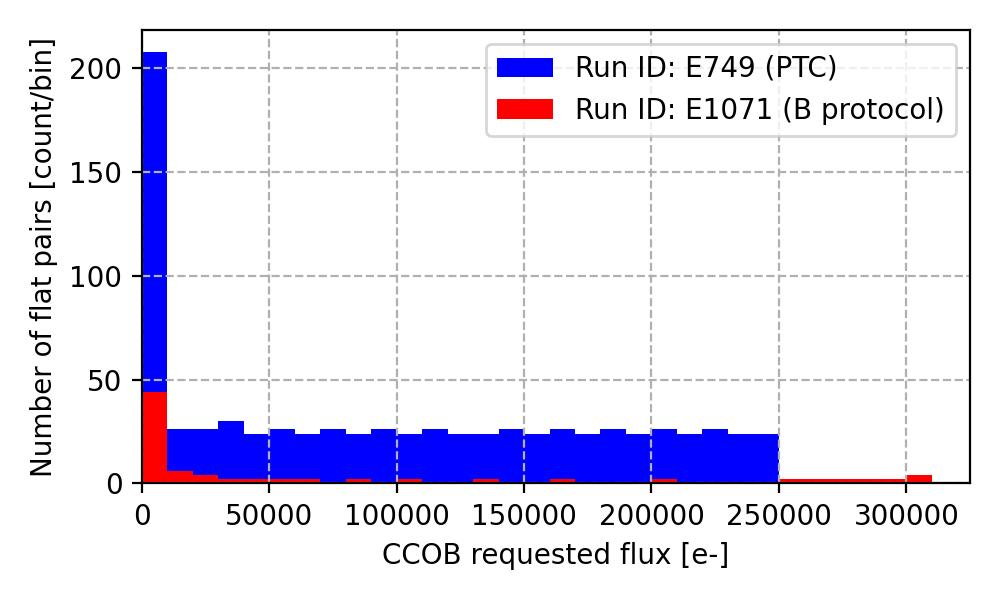
\includegraphics[width=0.7\textwidth]{figures/baselineCharacterization/PTC_BProtocol_Comparison.jpg}
	\caption{Flat-pair comparison between PTC and B protocol
\label{fig:PTC_BProtocol_Comparison}}
\end{centering}
\end{figure}

For comparisons between Cerro Pachon EO runs and the final SLAC IR2 equivalents, the following runs are used (see Table~\ref{runTable-b-ptc}).

\begin{table}[ht]
\centering
\caption{Reference runs for Run 6 and Run 7 comparisons} \label{runTable-b-ptc}
\begin{tabular}{lll}
\toprule
Run Type & Run 6 & Run 7 \\
\midrule
B Protocol & 13550 & E1071 \\
PTC        & 13591 & E749 \\
\bottomrule
\end{tabular}
\end{table}

The naming of the EO runs was established during initial LSST Camera
integration and testing. The final SLAC IR2 run from November 2023 was
named ``Run 6", while the data acquisitions from Cerro Pachon from September through December 2024 are considered ``Run 7". Additionally, individual EO acquisitions are tagged with a run identifier. This is commonly referred to as a Run ID. For all SLAC runs, the run identifier was a five digit numeric code, while the Cerro Pachon runs were ``E-numbers" that started with a capital E followed by a numeric code.


\subsection{Stability flat metrics}\label{stability-flat-metrics}

\subsubsection{Charge transfer
inefficiency}\label{charge-transfer-inefficiency}

CTI, or charge transfer inefficiency, measures the fraction of charge that fails to transfer from row to row during readout, and appears as trailing charge in the image area. Consequences of high CTI include loss of charge, distorted signals in the direction of parallel transfer, and reduced sensitivity in low light imaging. CTI measurements are made using the EPER method \citep{2021JATIS...7d8002S}, for which the ratio of the residual charge in the overscan pixels to the total signal charge in the imaging region is evaluated. In the context of LSST Camera, we measure CTI along both the serial and parallel directions.

\paragraph{Serial CTI}\label{serial-cti}

\begin{figure}[ht]
\begin{centering}
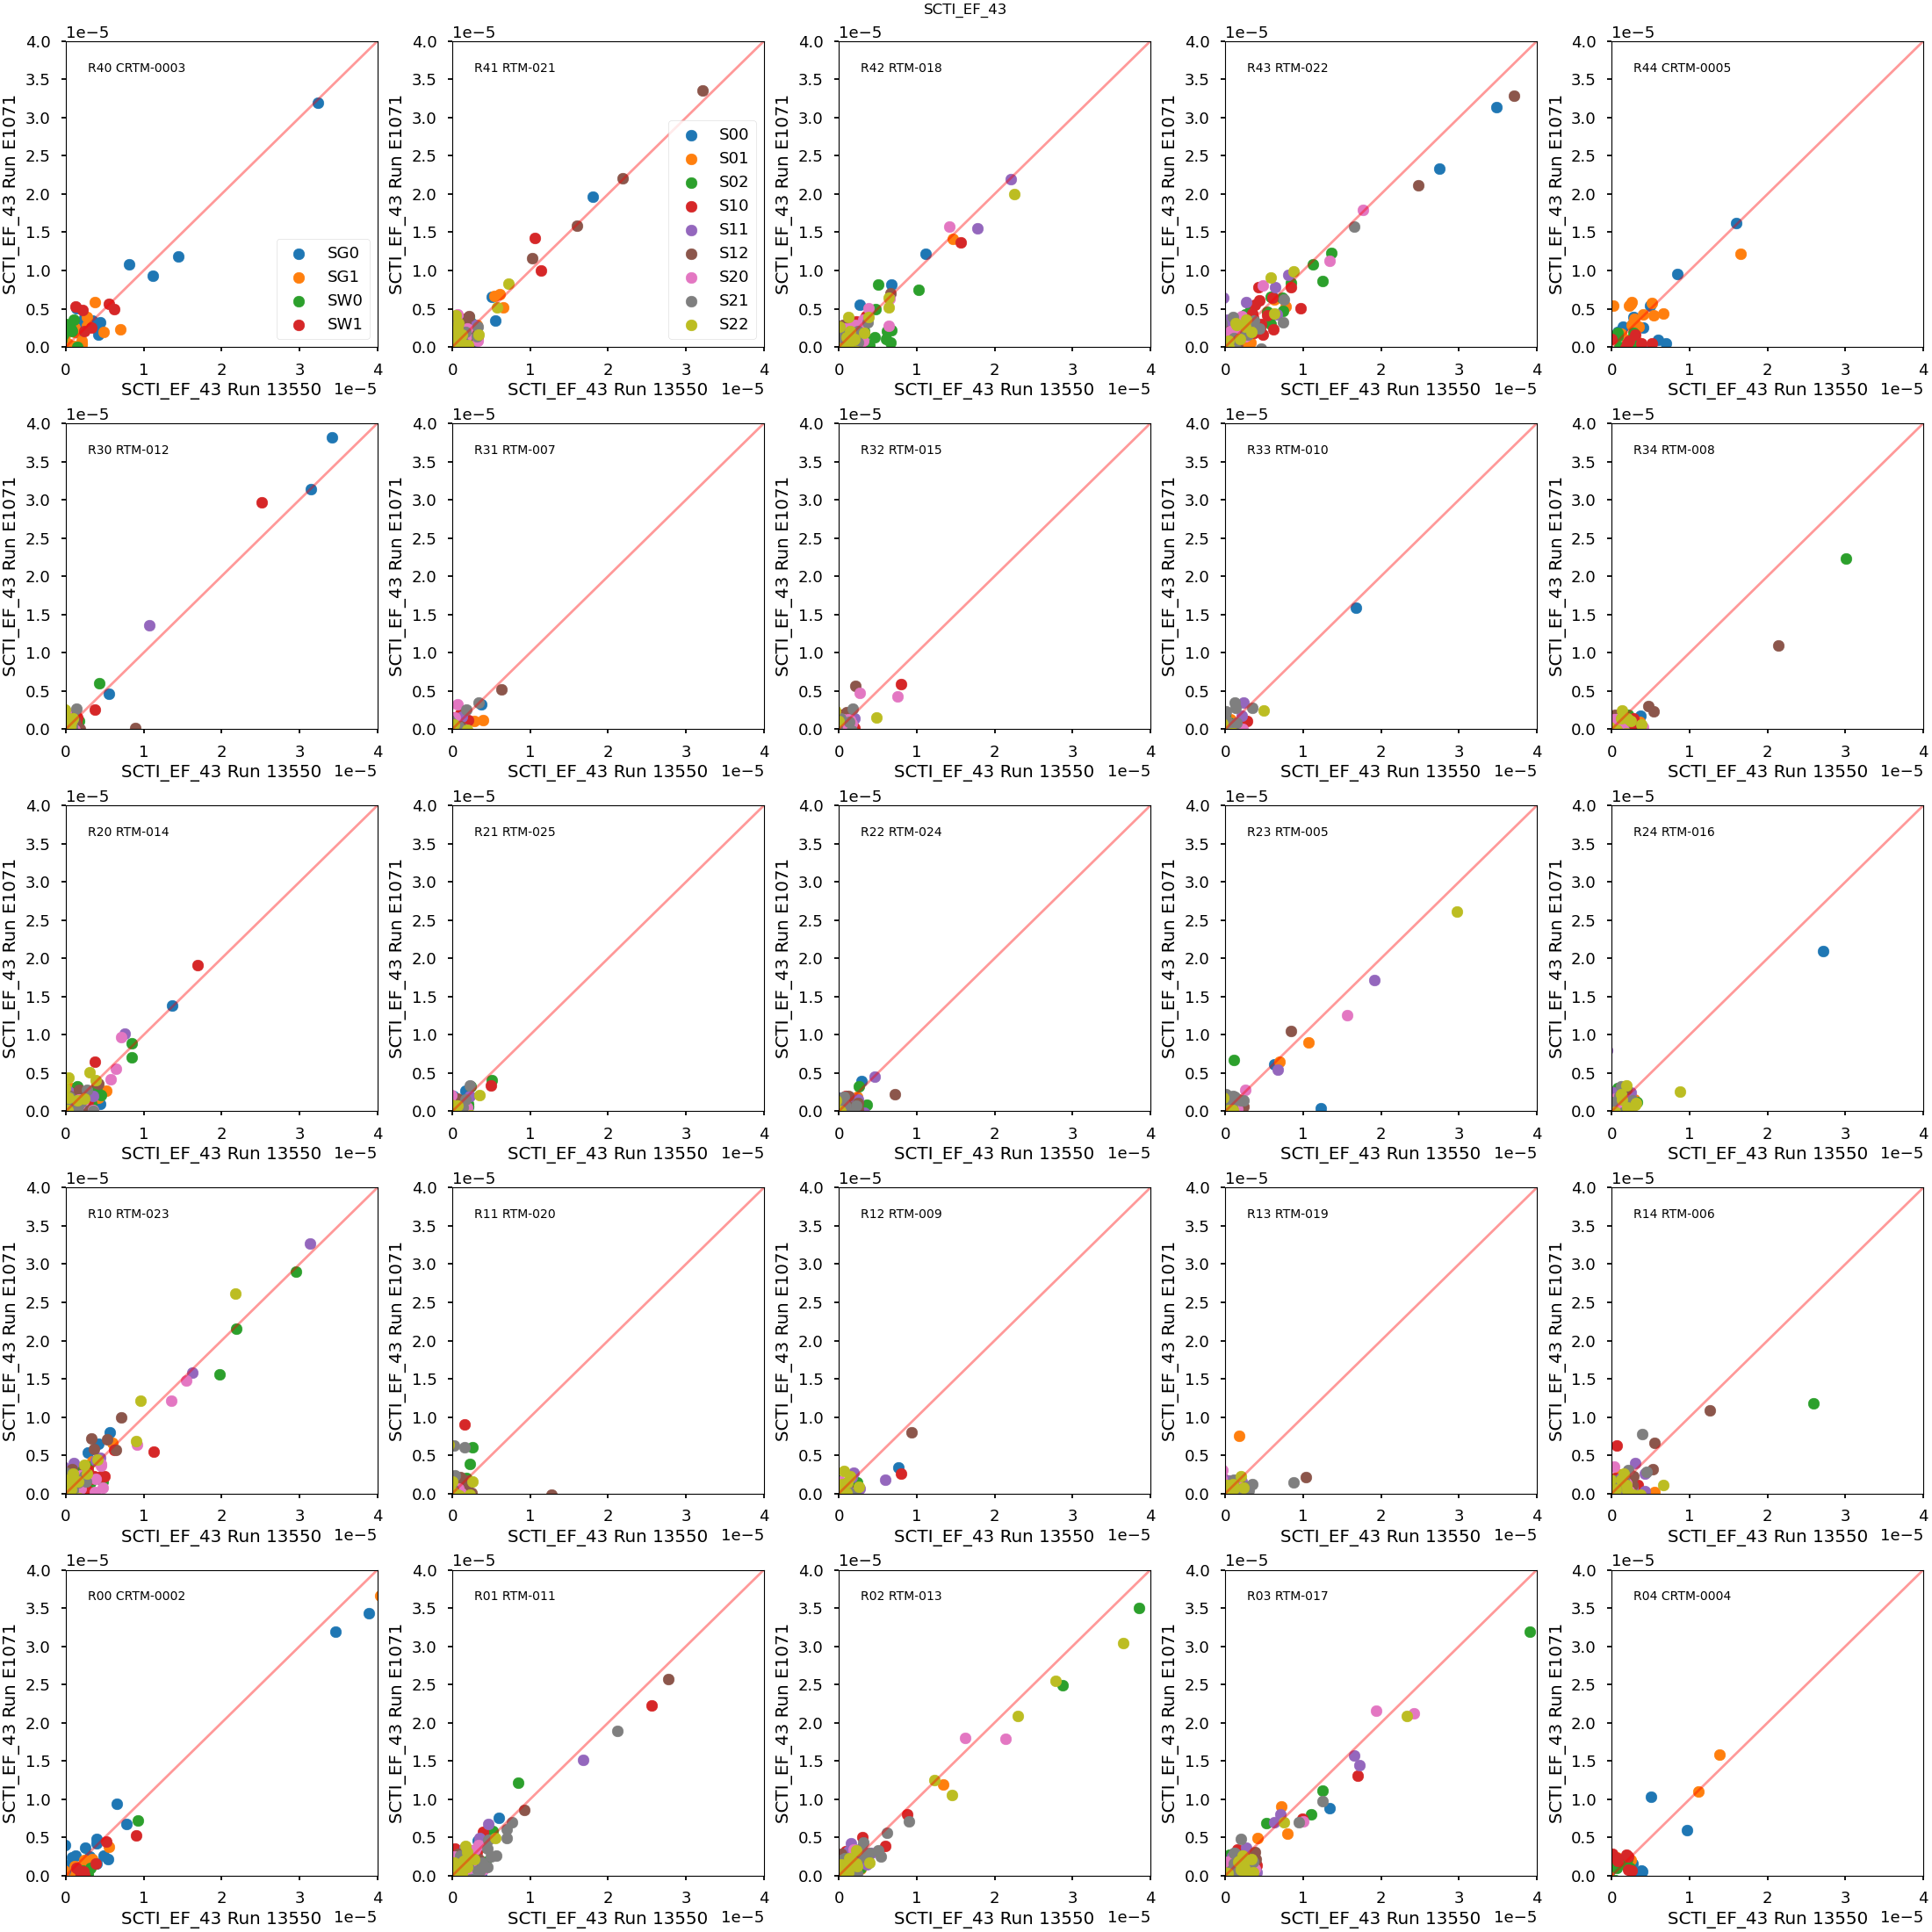
\includegraphics[width=0.7\textwidth]{figures/baselineCharacterization/13550_E1071_SCTI_EF_43_inset.png}
	\caption{Serial CTI amplifier measurements separated by raft for Run 7 (E1071) and Run 6 (13550)\label{fig:serial-cti}}
\end{centering}
\end{figure}

The CTI along the serial registers of the amplifier segments of the LSST Camera CCDs is consistent between Run 6 and
Run 7 (Fig.~\ref{fig:serial-cti}). Both sensor types show low CTI,
span a range  of \textasciitilde$2 \times 10^{-5}$ \% for e2v sensors, and
by \textasciitilde$4 \times 10^{-6}$  \% for ITL sensors (Fig.~\ref{fig:serial-cti-dist}). 

\begin{figure}[ht]
\begin{centering}
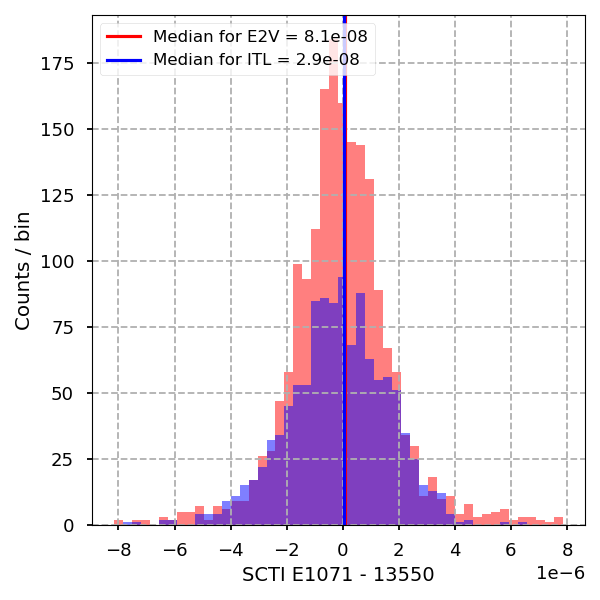
\includegraphics[width=0.7\textwidth]{figures/baselineCharacterization/SCTI_13550_E1071_diff.png}
\caption{Distributions of differences in serial charge transfer inefficiencies between Run 7 (E1071) and Run 6 (13550), grouped by CCD type.}
\label{fig:serial-cti-dist}
\end{centering}
\end{figure}

\clearpage
\paragraph{Parallel CTI}\label{parallel-cti}

The CTI along the parallel direction is consistent between Run 6 and
Run 7 (Fig.~\ref{fig:parallel-cti}). Both sensor types are found to have extremely low CTI on the order of $10^{-5}$ \%,
and span a range of \textasciitilde$1 \times 10^{-5}$ \% for e2v sensors, and
by \textasciitilde$7 \times 10^{-4}$ \% for ITL sensors (Fig.~\ref{fig:parallel-cti-dist}). Both of these measurements pass the CTI requirements (see table \ref{tab:initRever:Table}).

\begin{figure}[ht]
\begin{centering}
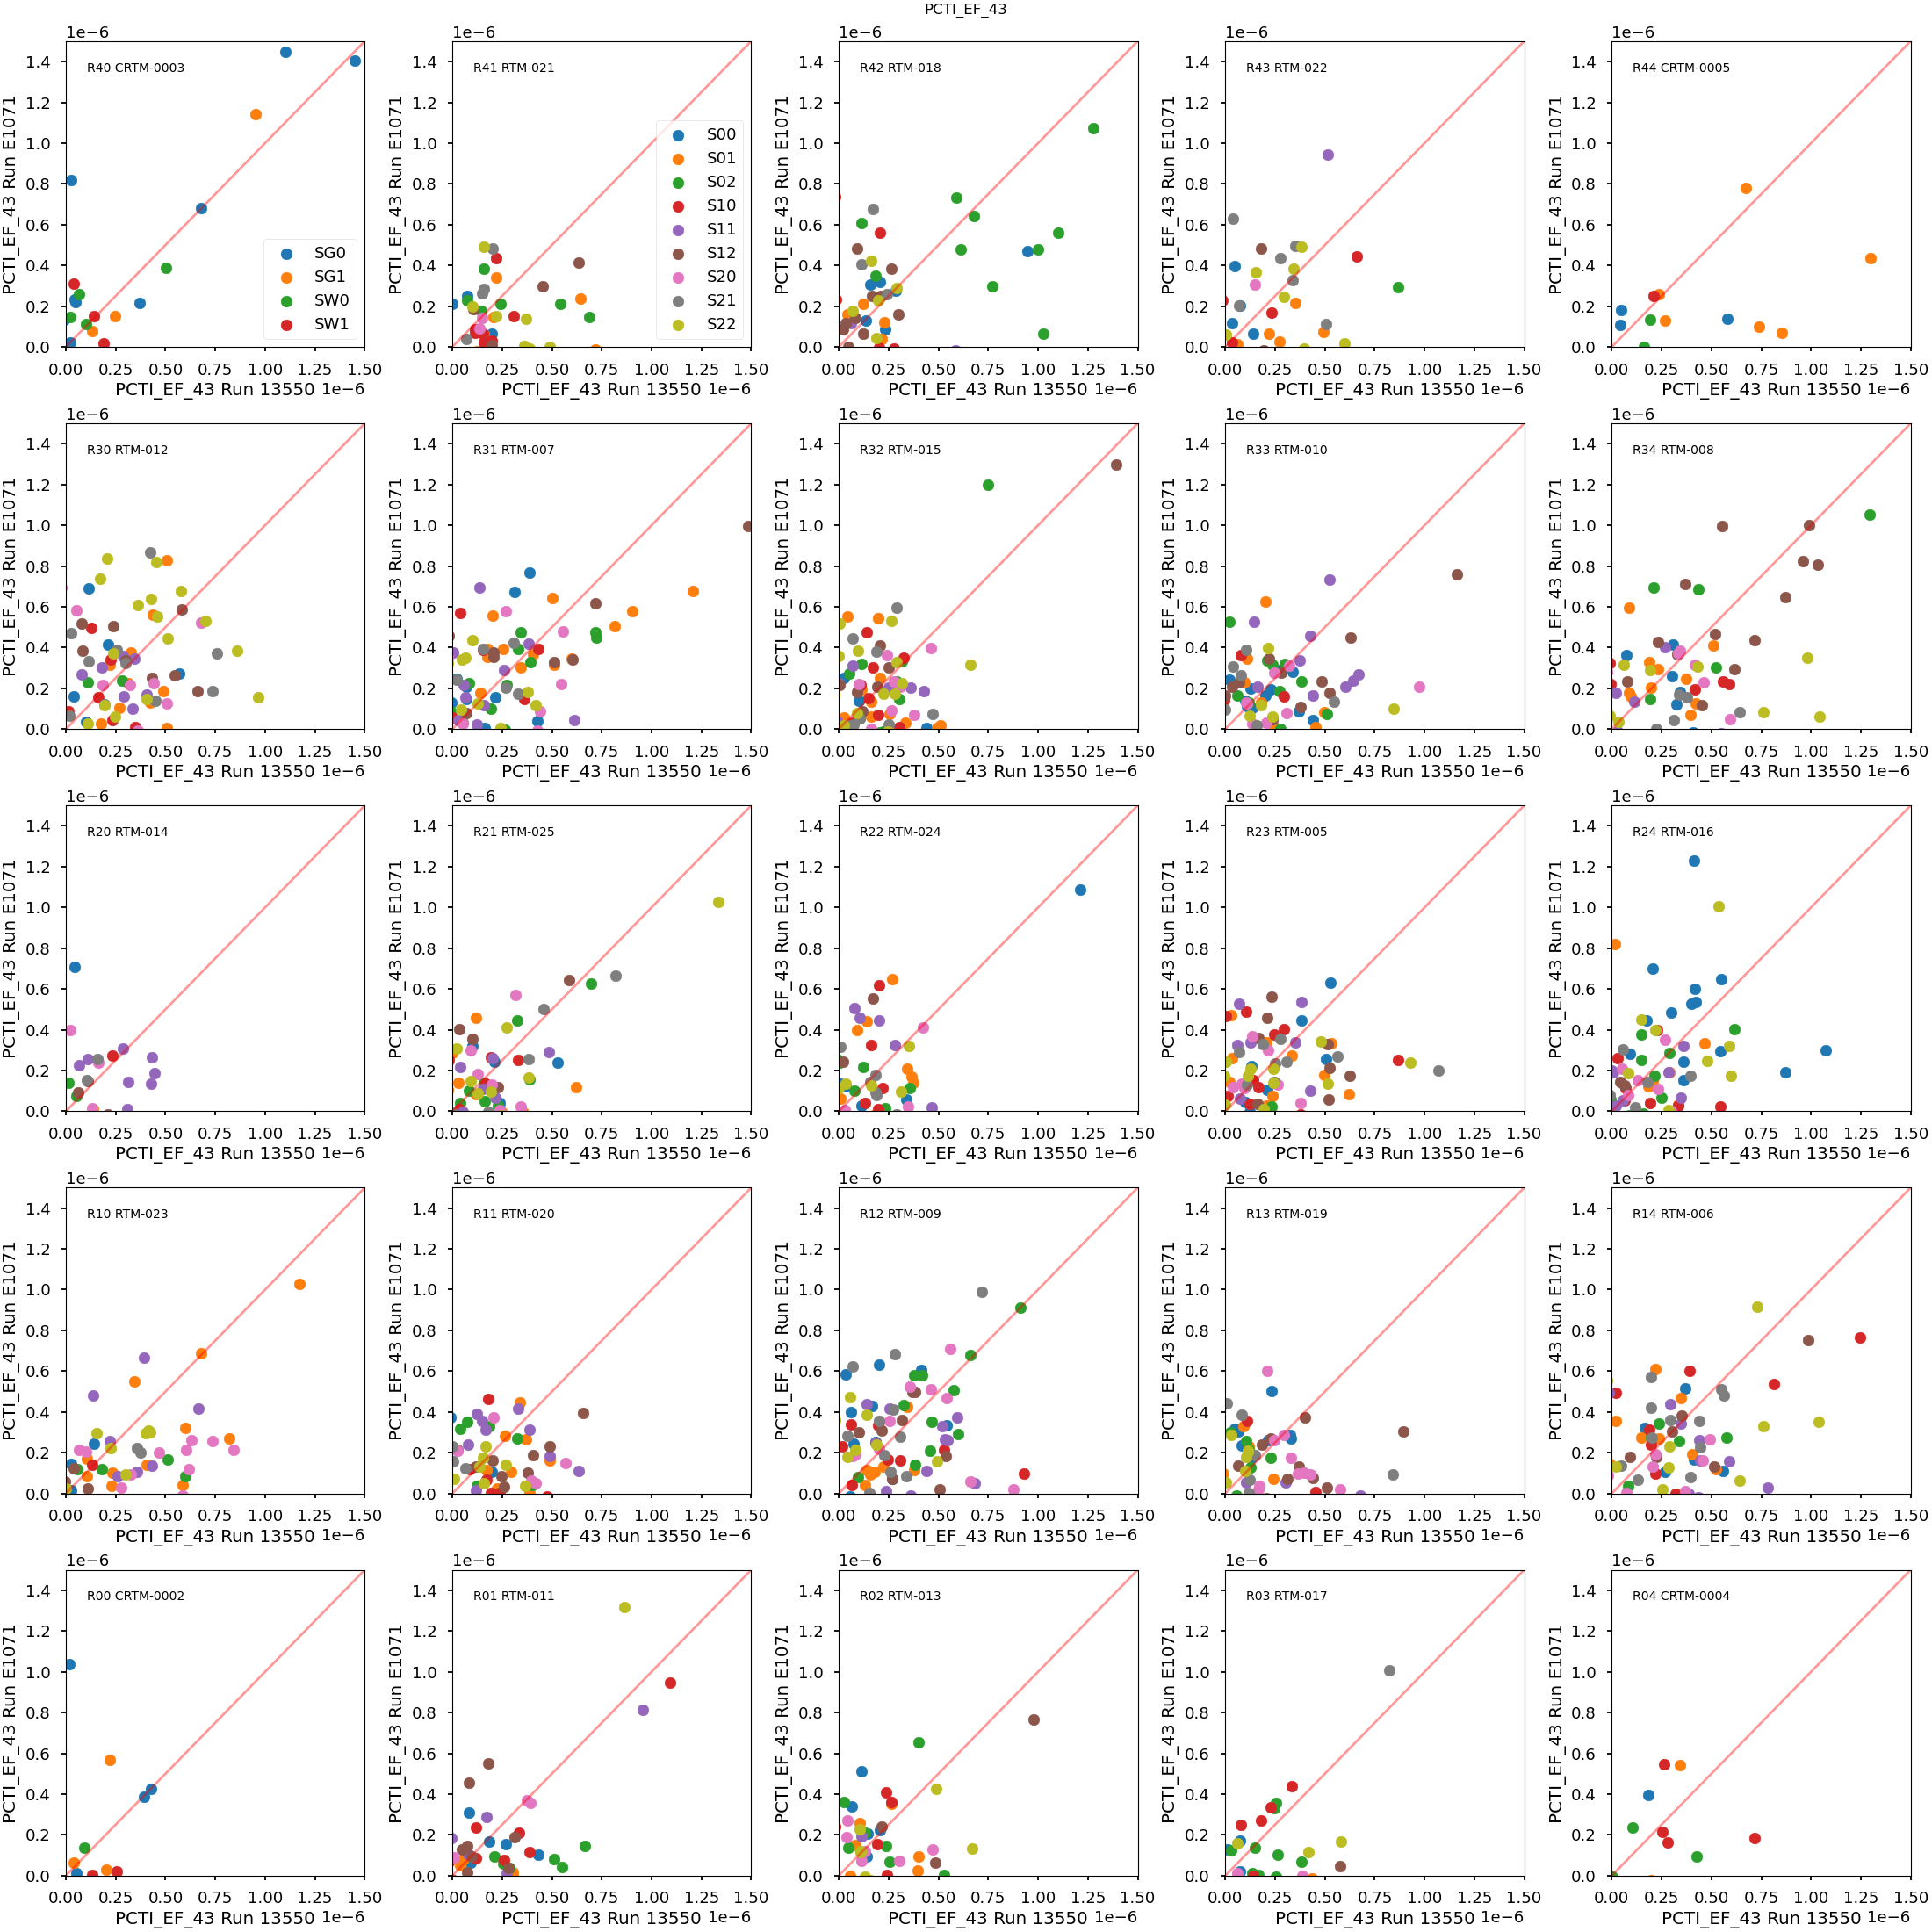
\includegraphics[width=0.7\textwidth]{figures/baselineCharacterization/13550_E1071_PCTI_EF_43_inset.png}
\caption{Parallel CTI comparison by raft for Run 7 (E1017) and Run 6 (13550).}
\label{fig:parallel-cti}
\end{centering}
\end{figure}

\begin{figure}[ht]
\begin{centering}
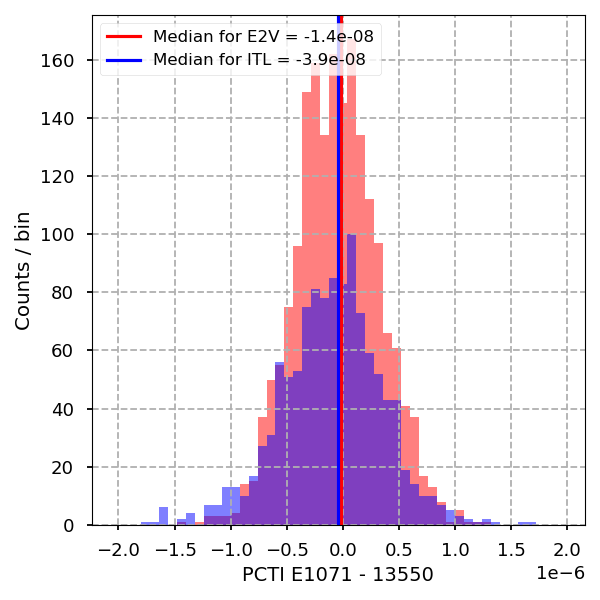
\includegraphics[width=0.7\textwidth]{figures/baselineCharacterization/PCTI_13550_E1071_diff.png}
\caption{Distributions of differences in parallel charge transfer inefficiencies between Run 7 (E1071) and Run 6 (13550), grouped by CCD type.}
\label{fig:parallel-cti-dist}
\end{centering}
\end{figure}

\clearpage
\subsection{Dark metrics}\label{dark-metrics}

\subsubsection{Dark current}\label{dark-current}

Dark current is the small amount of electrical charge generated in the
absence of light due to thermal activity within the semiconductor
material of a CCD. This effect occurs when electron/hole pairs are thermally released
into the conduction band in the CCD, mimicking the signal that light would
produce. Dark current increases with temperature, so cooling the CCD is
a common method to reduce it in sensitive imaging applications. Dark
current introduces noise into an image, particularly in low-sky background conditions in long exposures.
The measurement of dark includes the dark current and stray light, making them impossible to distinguish each other since they both linearly evolve with time.
In the context
of LSST Camera, we measure dark current from the combined dark images across
all amplifiers as the upper limit.

\begin{figure}[ht]
\begin{centering}
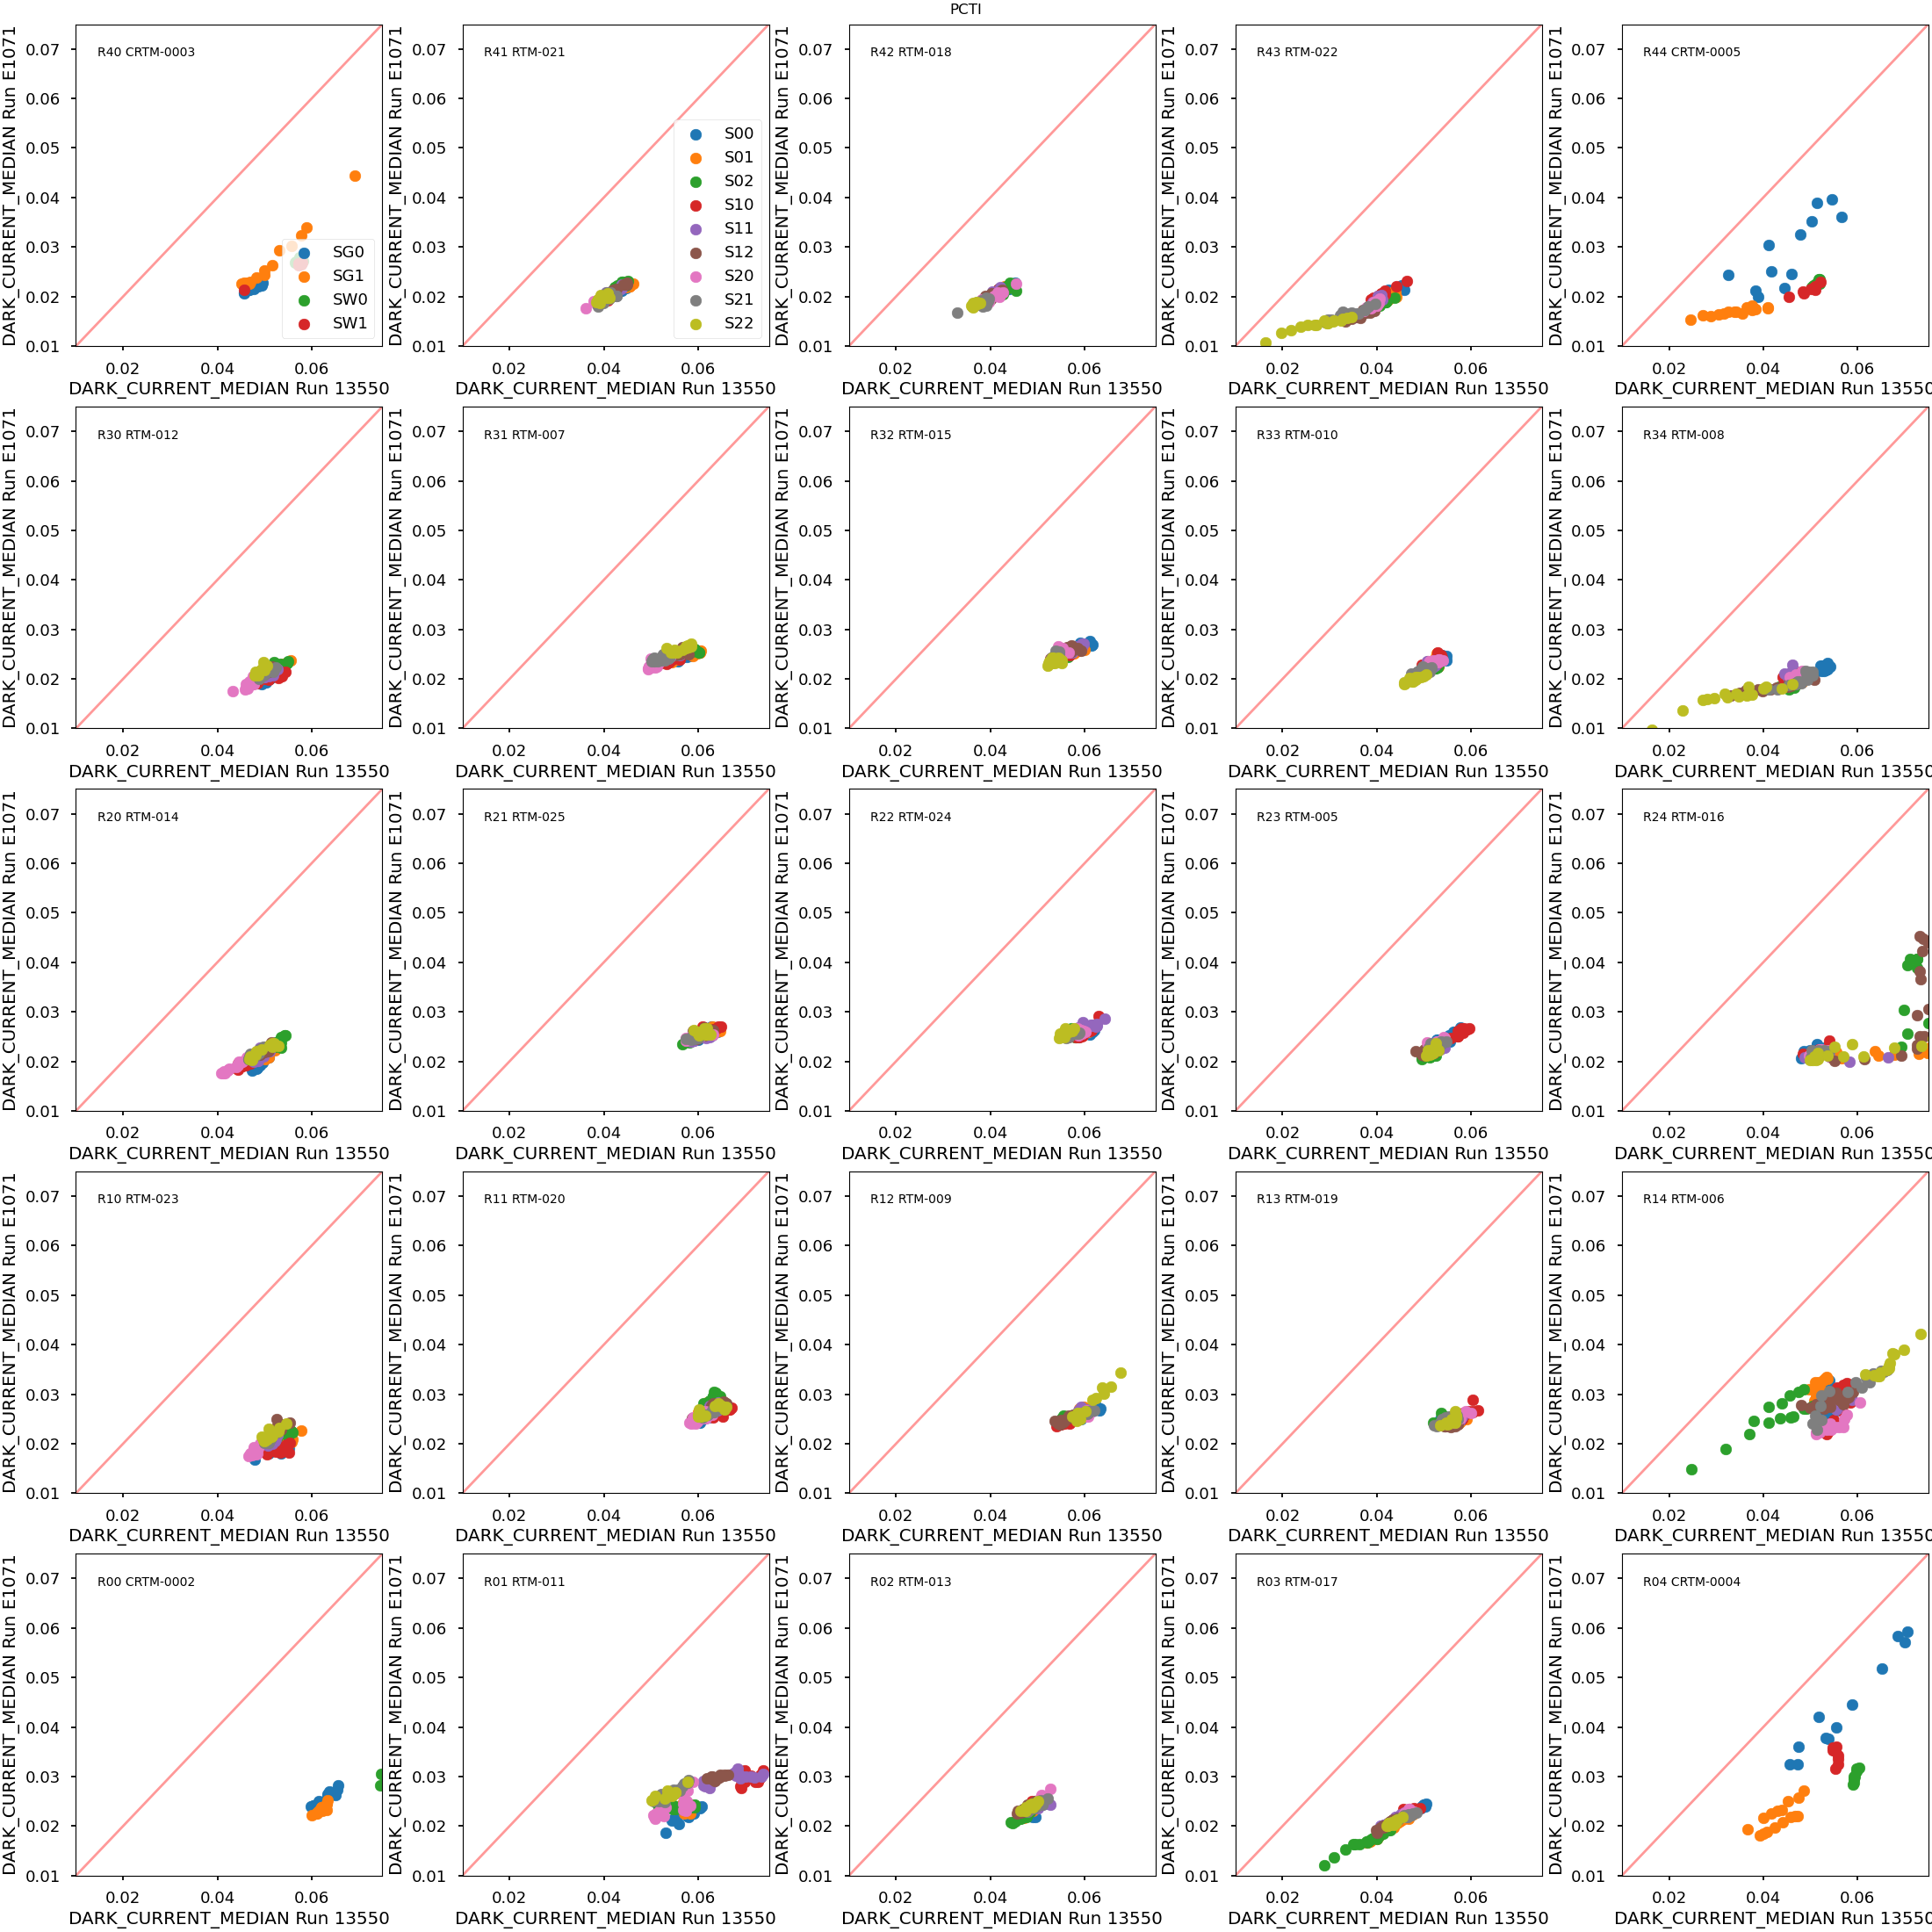
\includegraphics[width=0.7\textwidth]{figures/baselineCharacterization/13550_E1071_DARK_CURRENT_MEDIAN_inset.png}
\caption{Dark current comparison by raft for Run 7 (E1071) and Run 6 (13550).}
\label{fig:dark}
\end{centering}
\end{figure}

Unexpectedly, the dark current was significantly less in Run 7 than
Run 6 (Fig.~\ref{fig:dark}). We do not attach particular significance to the finding because this could be the result of improved shrouding on the camera in the Level 3 white room relative to the IR2 clean room SLAC.

\clearpage
\subsubsection{Bright defects}\label{bright-defects}

Bright defects are localized regions or individual pixels that produce abnormally high signal levels, even in the absence of light. These defects are typically caused by imperfections in the semiconductor material or manufacturing process of the CCD. Bright defects can manifest as ``hot pixels" with consistently high dark current, small clusters of pixels with elevated dark current, or as ``hot columns" (pixels along the same column that have high dark current). 

In the context of LSST Camera, we identify and exclude bright pixels from the dark current measurement, with the threshold for a bright defect set at 5 e$^-$/pix/s, above which the pixel/cluster/column is registered as a bright defect. In addition to the bright pixel metric, eo-pipe also computes a bright column metric, which is any region of bright pixels that is contiguous over 50 pixels or more.

\begin{figure}[ht]
\begin{centering}
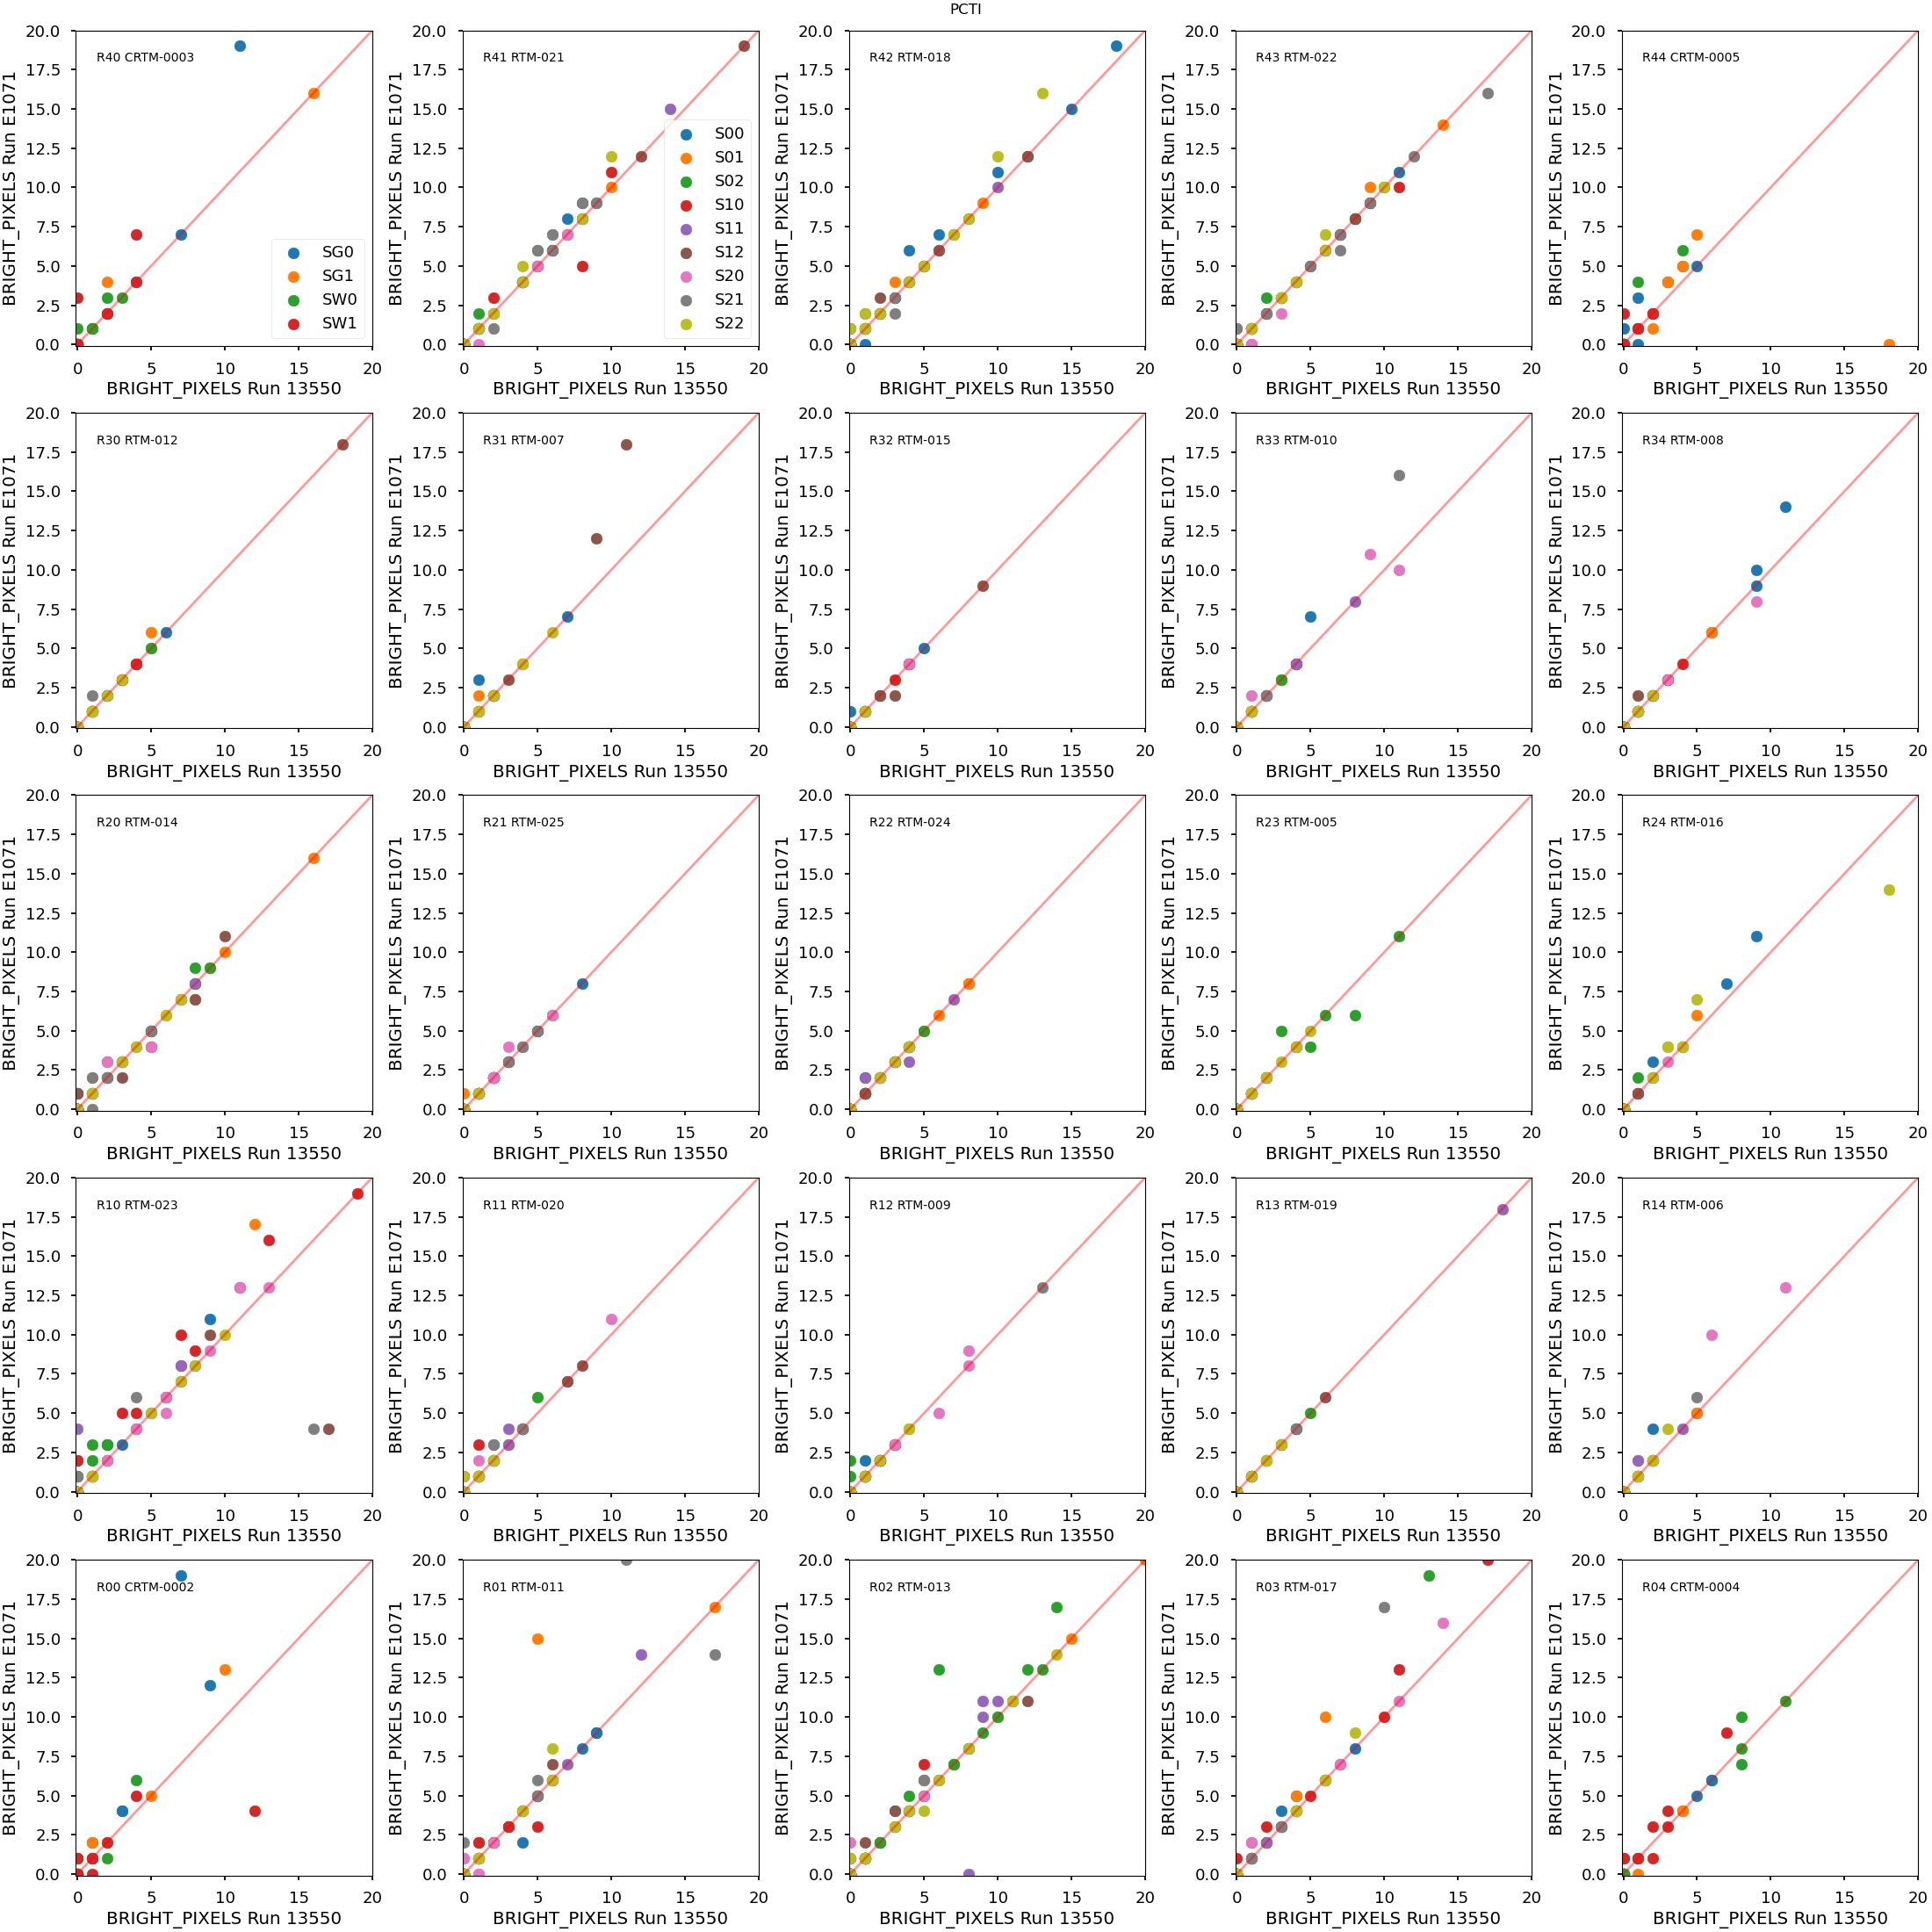
\includegraphics[width=0.7\textwidth]{figures/baselineCharacterization/13550_E1071_BRIGHT_PIXELS_inset.png}
\caption{Bright pixel comparison by raft for Run 7 (E1071) and Run 6 (13550)}
\label{fig:bright}
\end{centering}
\end{figure}

Evaluating the change in defect counts on each amplifier segment between Run 6 and Run 7, and aggregating the amplifiers by the detector manufacturer shows a small increase of bright defects in Run 7 (Fig.~\ref{fig:bright}). Figure~\ref{fig:dark-dist}) displays differences of the measurements. The median values agree well, while there are signs of the positive tail. For ITL sensors, we find that 12\% of the amplifiers have more bright pixels than in Run 6. For e2v sensors, we find 4\% of the amplifiers that have more bright pixels. Despite this, the number of bright defects between runs does not increase for most sensors.

The reason is not totally clear, but the difference in the illumination pattern as described in Section \ref{run-7-optical-modifications} might play a role, which implies that a small number of defects could be created in the CCOB optical path.

\begin{figure}[ht]
\begin{centering}
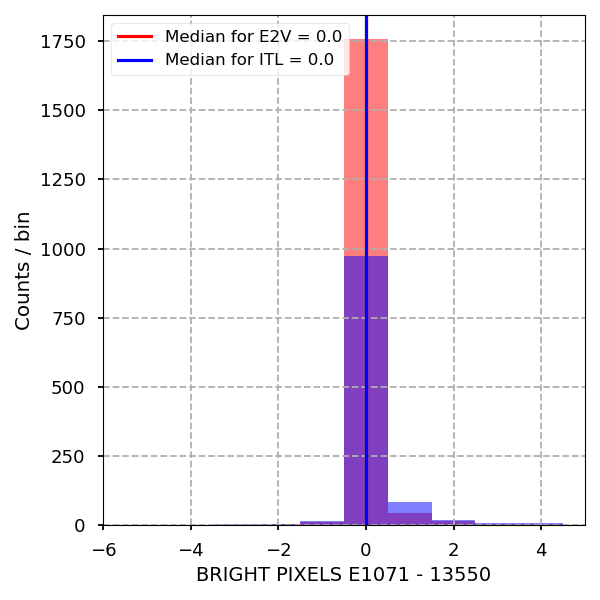
\includegraphics[width=0.7\textwidth]{figures/baselineCharacterization/BRIGHT_PIXELS_13550_E1071_diff.png}
\caption{Distributions of differences in bright pixel count per amplifier between Run 7 (E1071) and Run 6 (13550), grouped by CCD type.}
\label{fig:dark-dist}
\end{centering}
\end{figure}

\clearpage
\subsection{Flat pair metrics}\label{flat-pair-metrics}
\begin{figure}[ht]
\begin{centering}
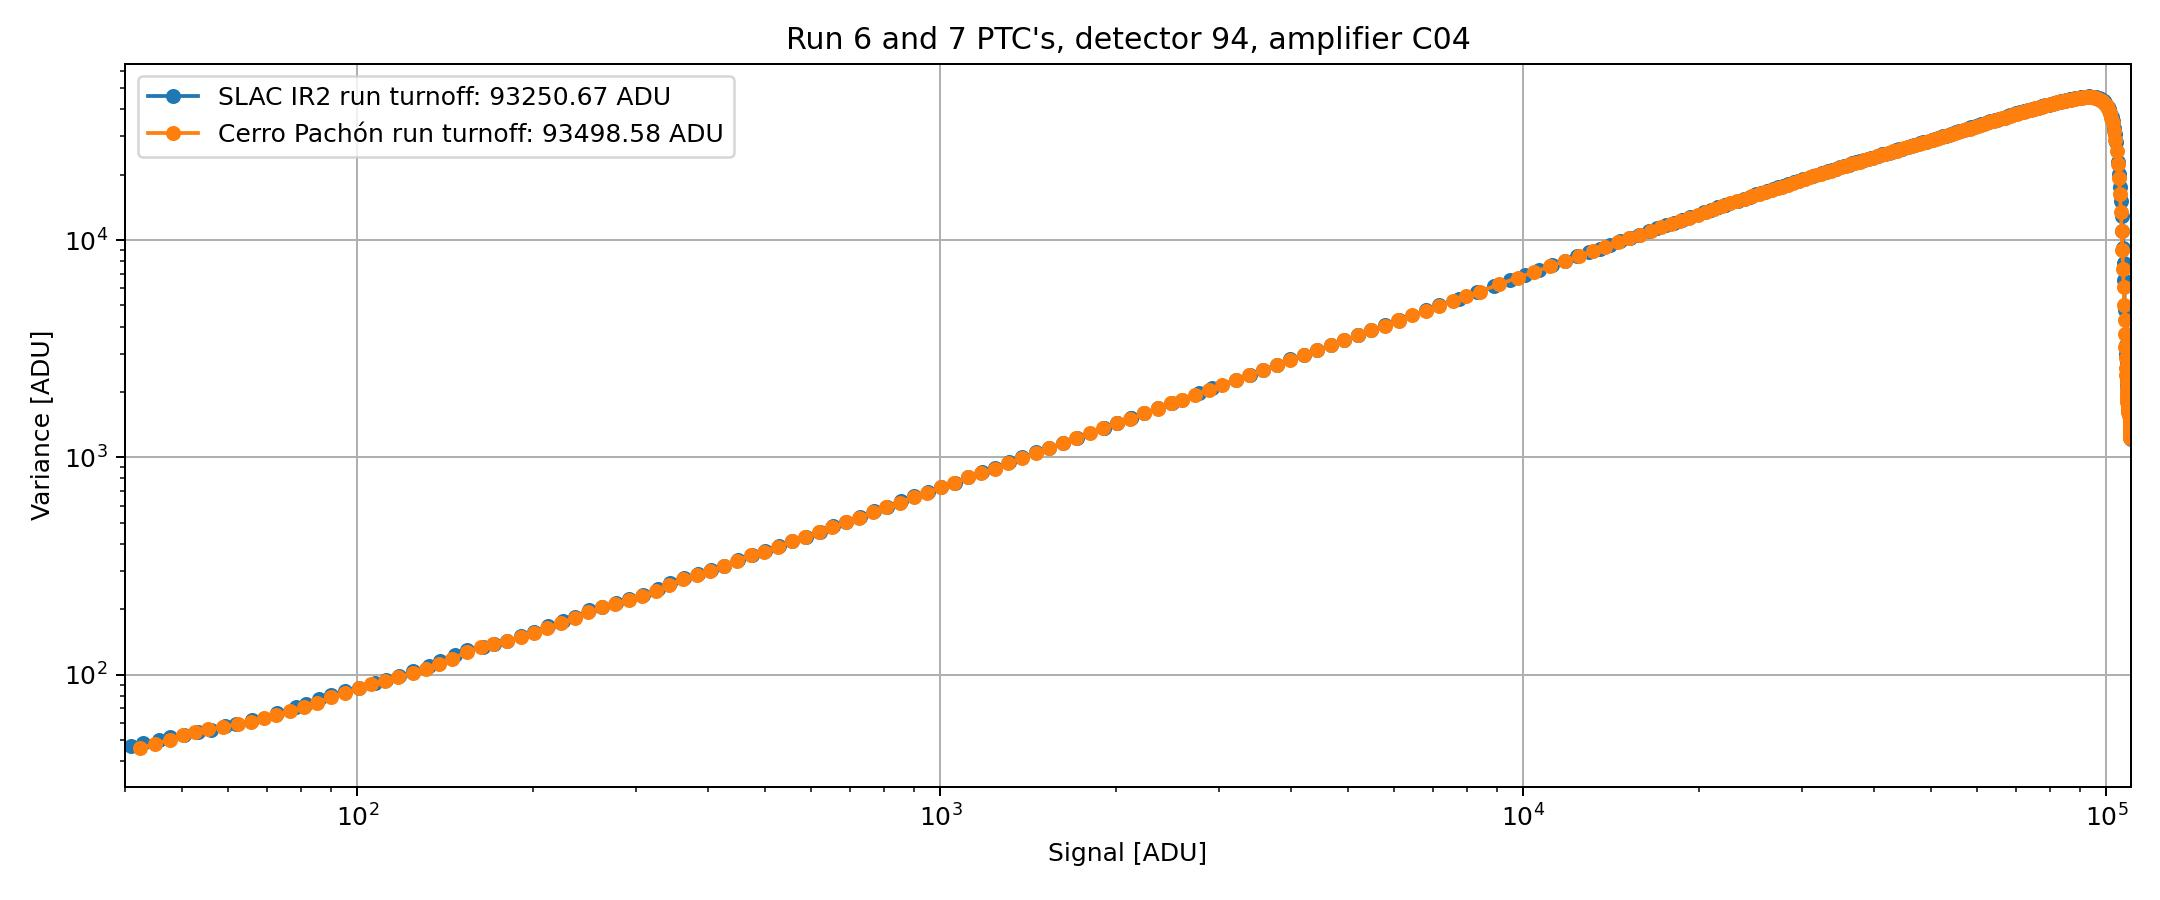
\includegraphics[width=0.95\textwidth]{figures/baselineCharacterization/run7PTCsToDate.jpg}
\caption{A comparison of Run 6 and Run 7 PTCs for a central amplifier.}
\label{fig:initRever:PTC_Comparison}
\end{centering}
\end{figure}

\subsubsection{Linearity and PTC turnoff}\label{linearity-and-ptc-turnoff}

Linearity turnoff and PTC turnoff are two closely related metrics used
to characterize the upper limit of the usable signal range for accurate shape measurements and photometry. Linearity turnoff is the signal level above which the PTC curve (Figure \ref{fig:initRever:PTC_Comparison}) deviates from
linearity and is measured for each amplifier segment of each CCD. We have defined the deviation threshold as 2\%.
PTC turnoff refers to the high-signal region of the PTC above which the PTC
variance decreases with increasing signal. This is due to saturation within the pixel wells of the CCDs. While slightly different, both metrics
provide important information about the upper limits of the dynamic
range in our sensors. Linearity turnoff is measured in units of e$^-$,
while PTC turnoff is measured in ADU.

\begin{figure}[ht]
\begin{centering}
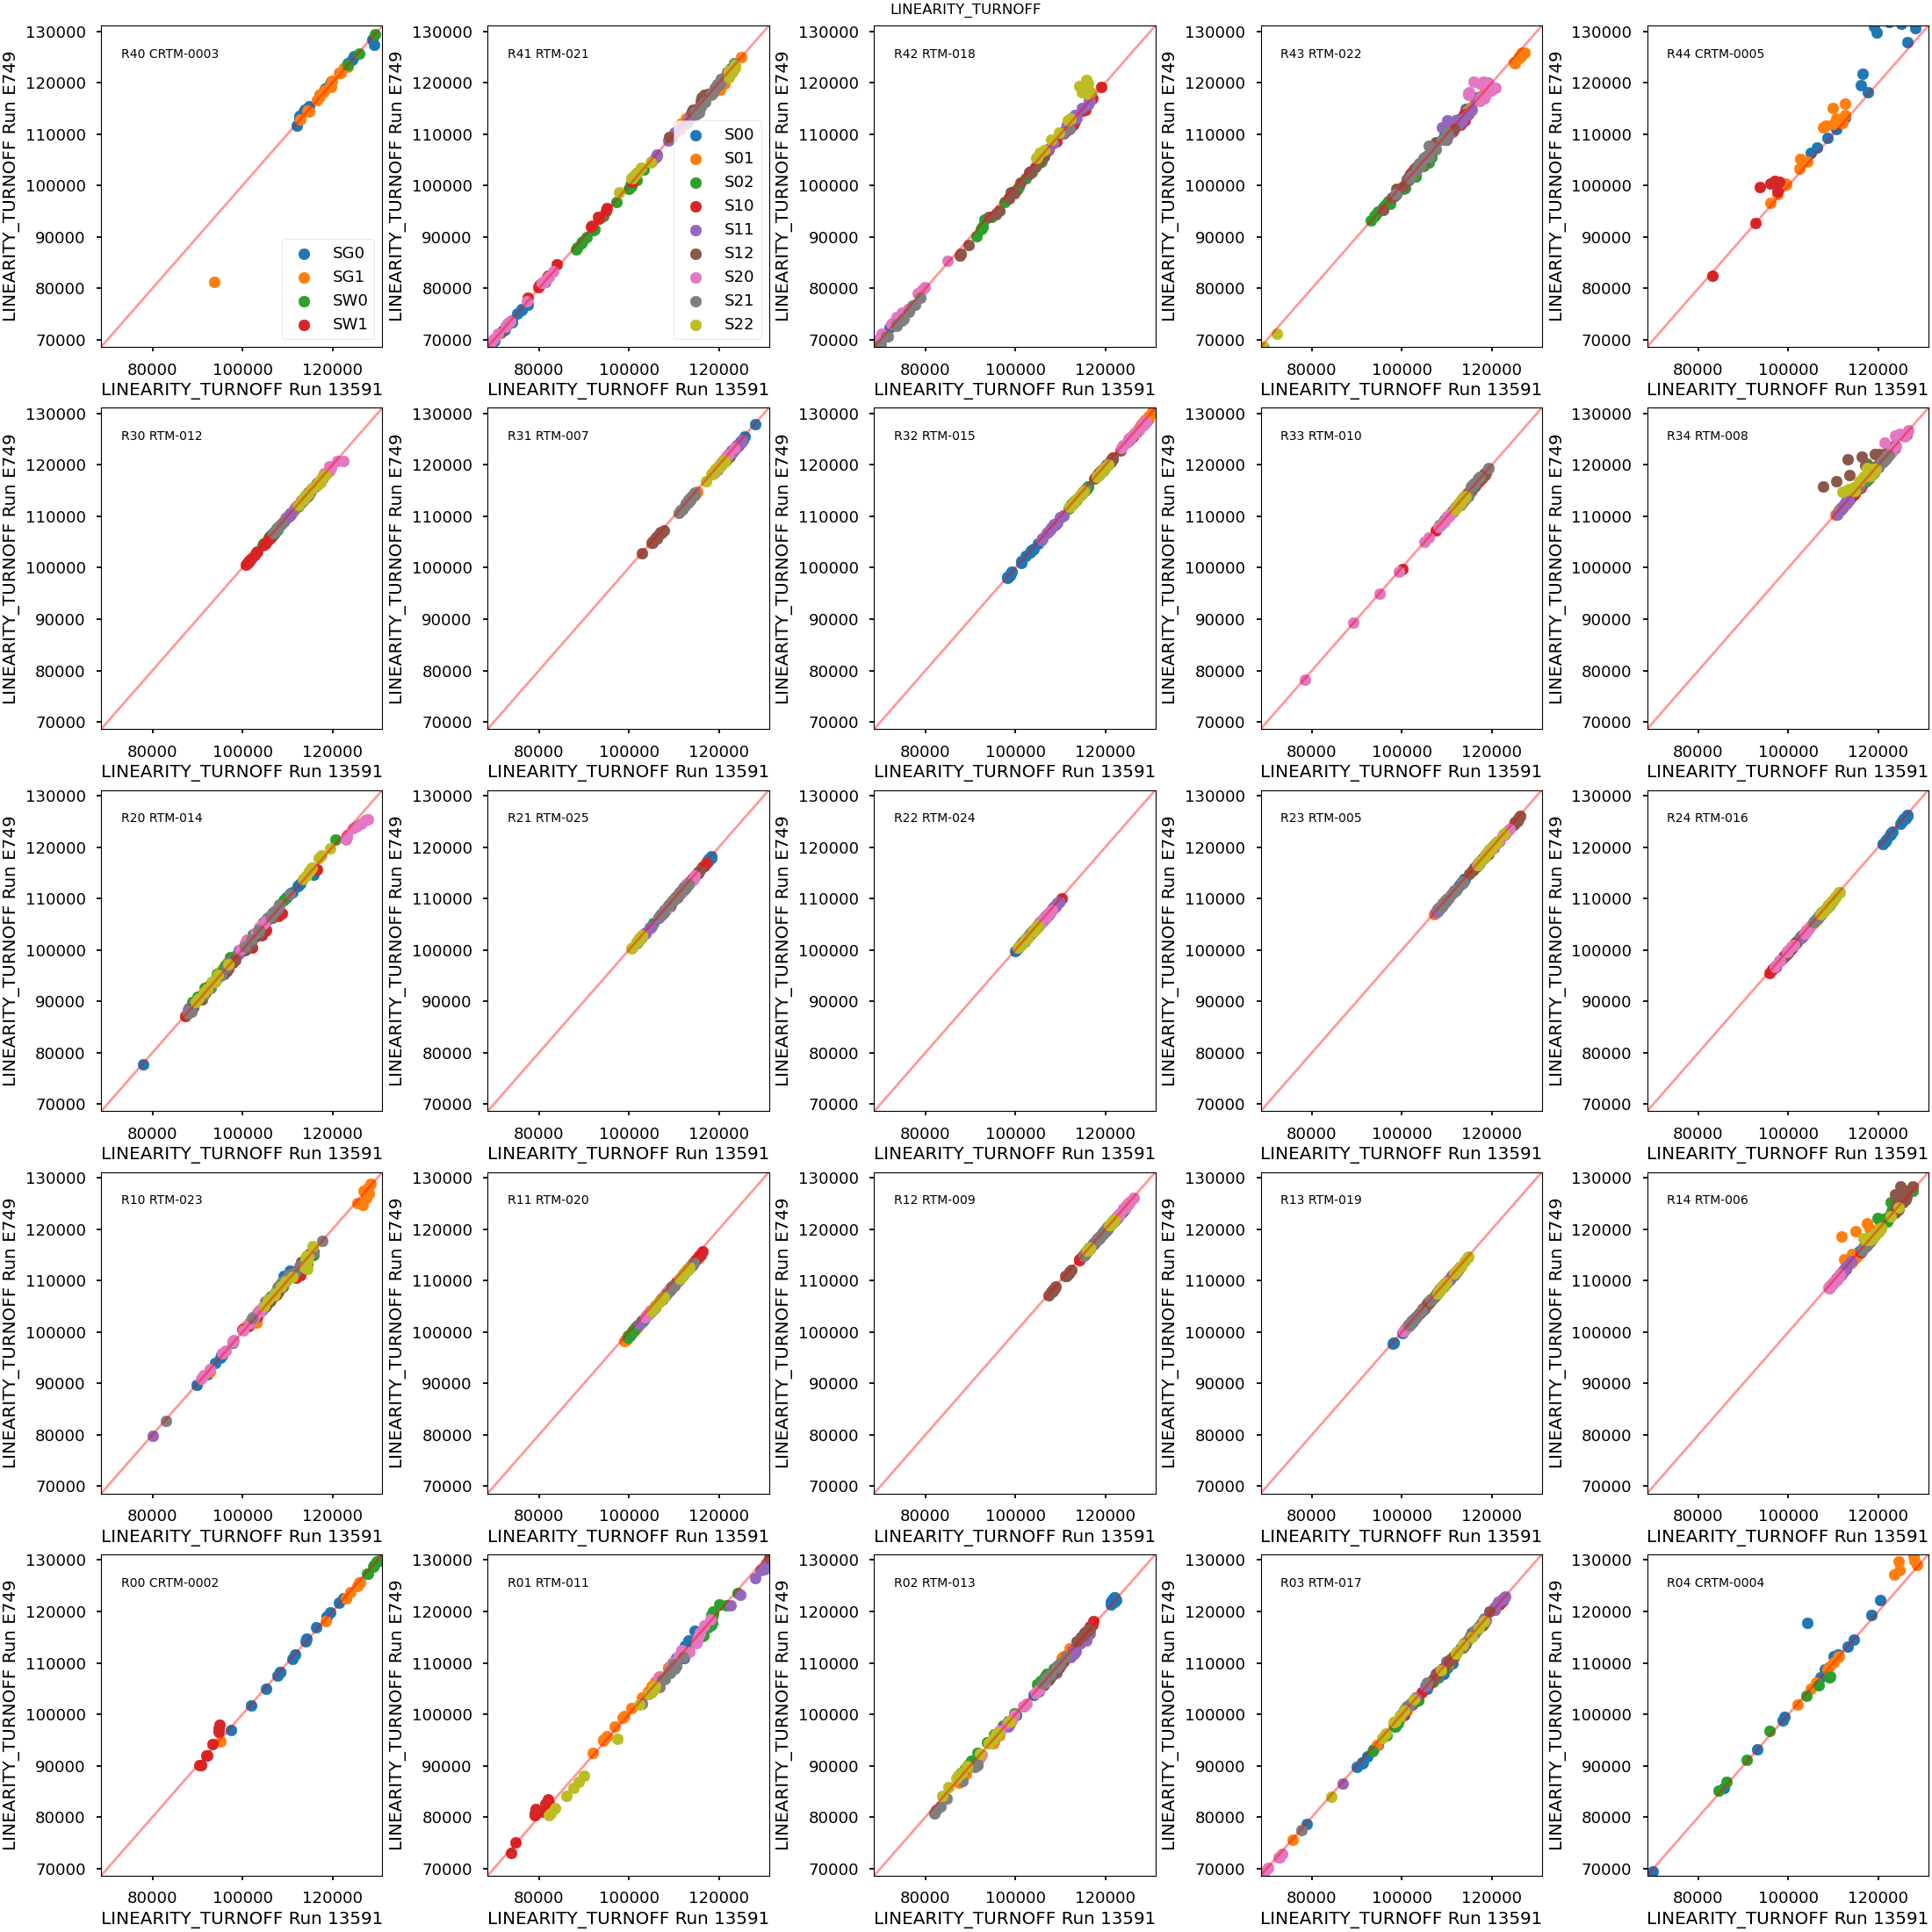
\includegraphics[width=0.7\textwidth]{figures/baselineCharacterization/13591_E749_LINEARITY_TURNOFF.png}
\caption{A comparison of Run 7 amplifier measurements of linearity turnoff, separated by sensor type. For both sensor types, measurements agree across both runs.}
\end{centering}
\end{figure}

In our linearity turnoff measurements, we find close agreement between
our Run 7 and Run 6 measurements for both ITL and e2v sensors.

\begin{figure}[ht]
\begin{centering}
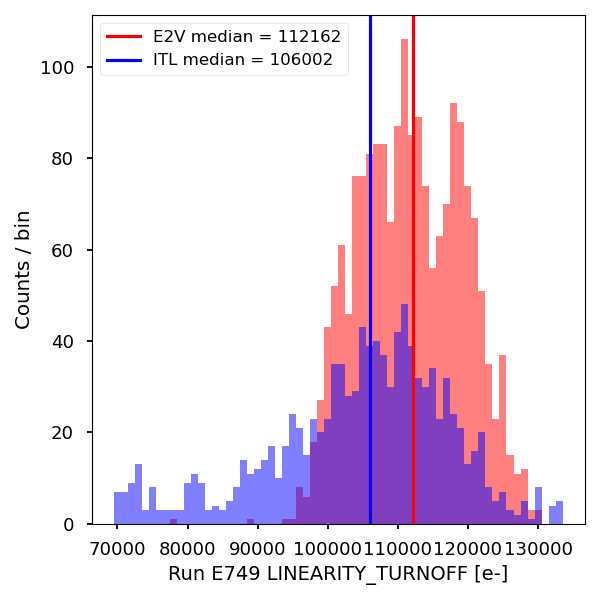
\includegraphics[width=0.7\textwidth]{figures/baselineCharacterization/LINEARITY_TURNOFF_E749_sensorType.png}
\caption{A comparison of Run 7 amplifier measurements of linearity turnoff, separated by sensor type. For both sensor types, linearity turnoff is above the 90k e- specification for a majority of amplifiers. A subset of ITL amplifiers are below the 90k e- threshold, while two e2v amplifiers are below that specification.}
\end{centering}
\end{figure}

Run 7 PTC turnoff measurements agree closely between Run 6 and Run 7, differing by $\leq$ 200 $e^-$ for both ITL and e2v sensors. Notably, they are lower on average for both detector types.

\begin{figure}[ht]
\begin{centering}
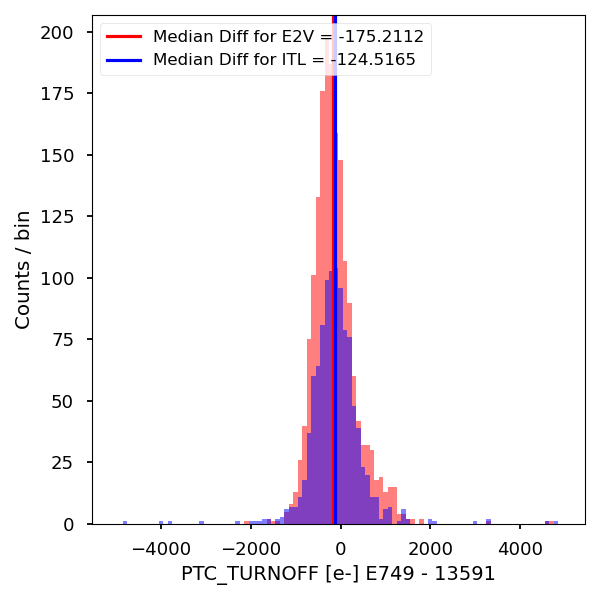
\includegraphics[width=0.7\textwidth]{figures/baselineCharacterization/PTC_TURNOFF_13591_E749_diff.png}
\caption{A comparison of Run 6 and Run 7 amplifier differences in PTC turnoff, separated by sensor type. For both sensor types, PTC turnoff is very consistent.}
\end{centering}
\end{figure}

\clearpage
\subsubsection{PTC gain}\label{ptc-gain}

PTC gain is the conversion factor between digital output signal and the the number of electrons generated in the pixels of the CCD. It is one of the key parameters derived from the Photon Transfer
Curve, as it is the slope above the flux range at which the variance is dominated by shot noise, and below the PTC turnoff. Gain is expressed in e$^-$/ADU, and scales the digitized analog signals from the ASPICs (Application Specific Photonic Integrated Circuits) to units of e$^{-1}$.

\begin{figure}[ht]
\begin{centering}
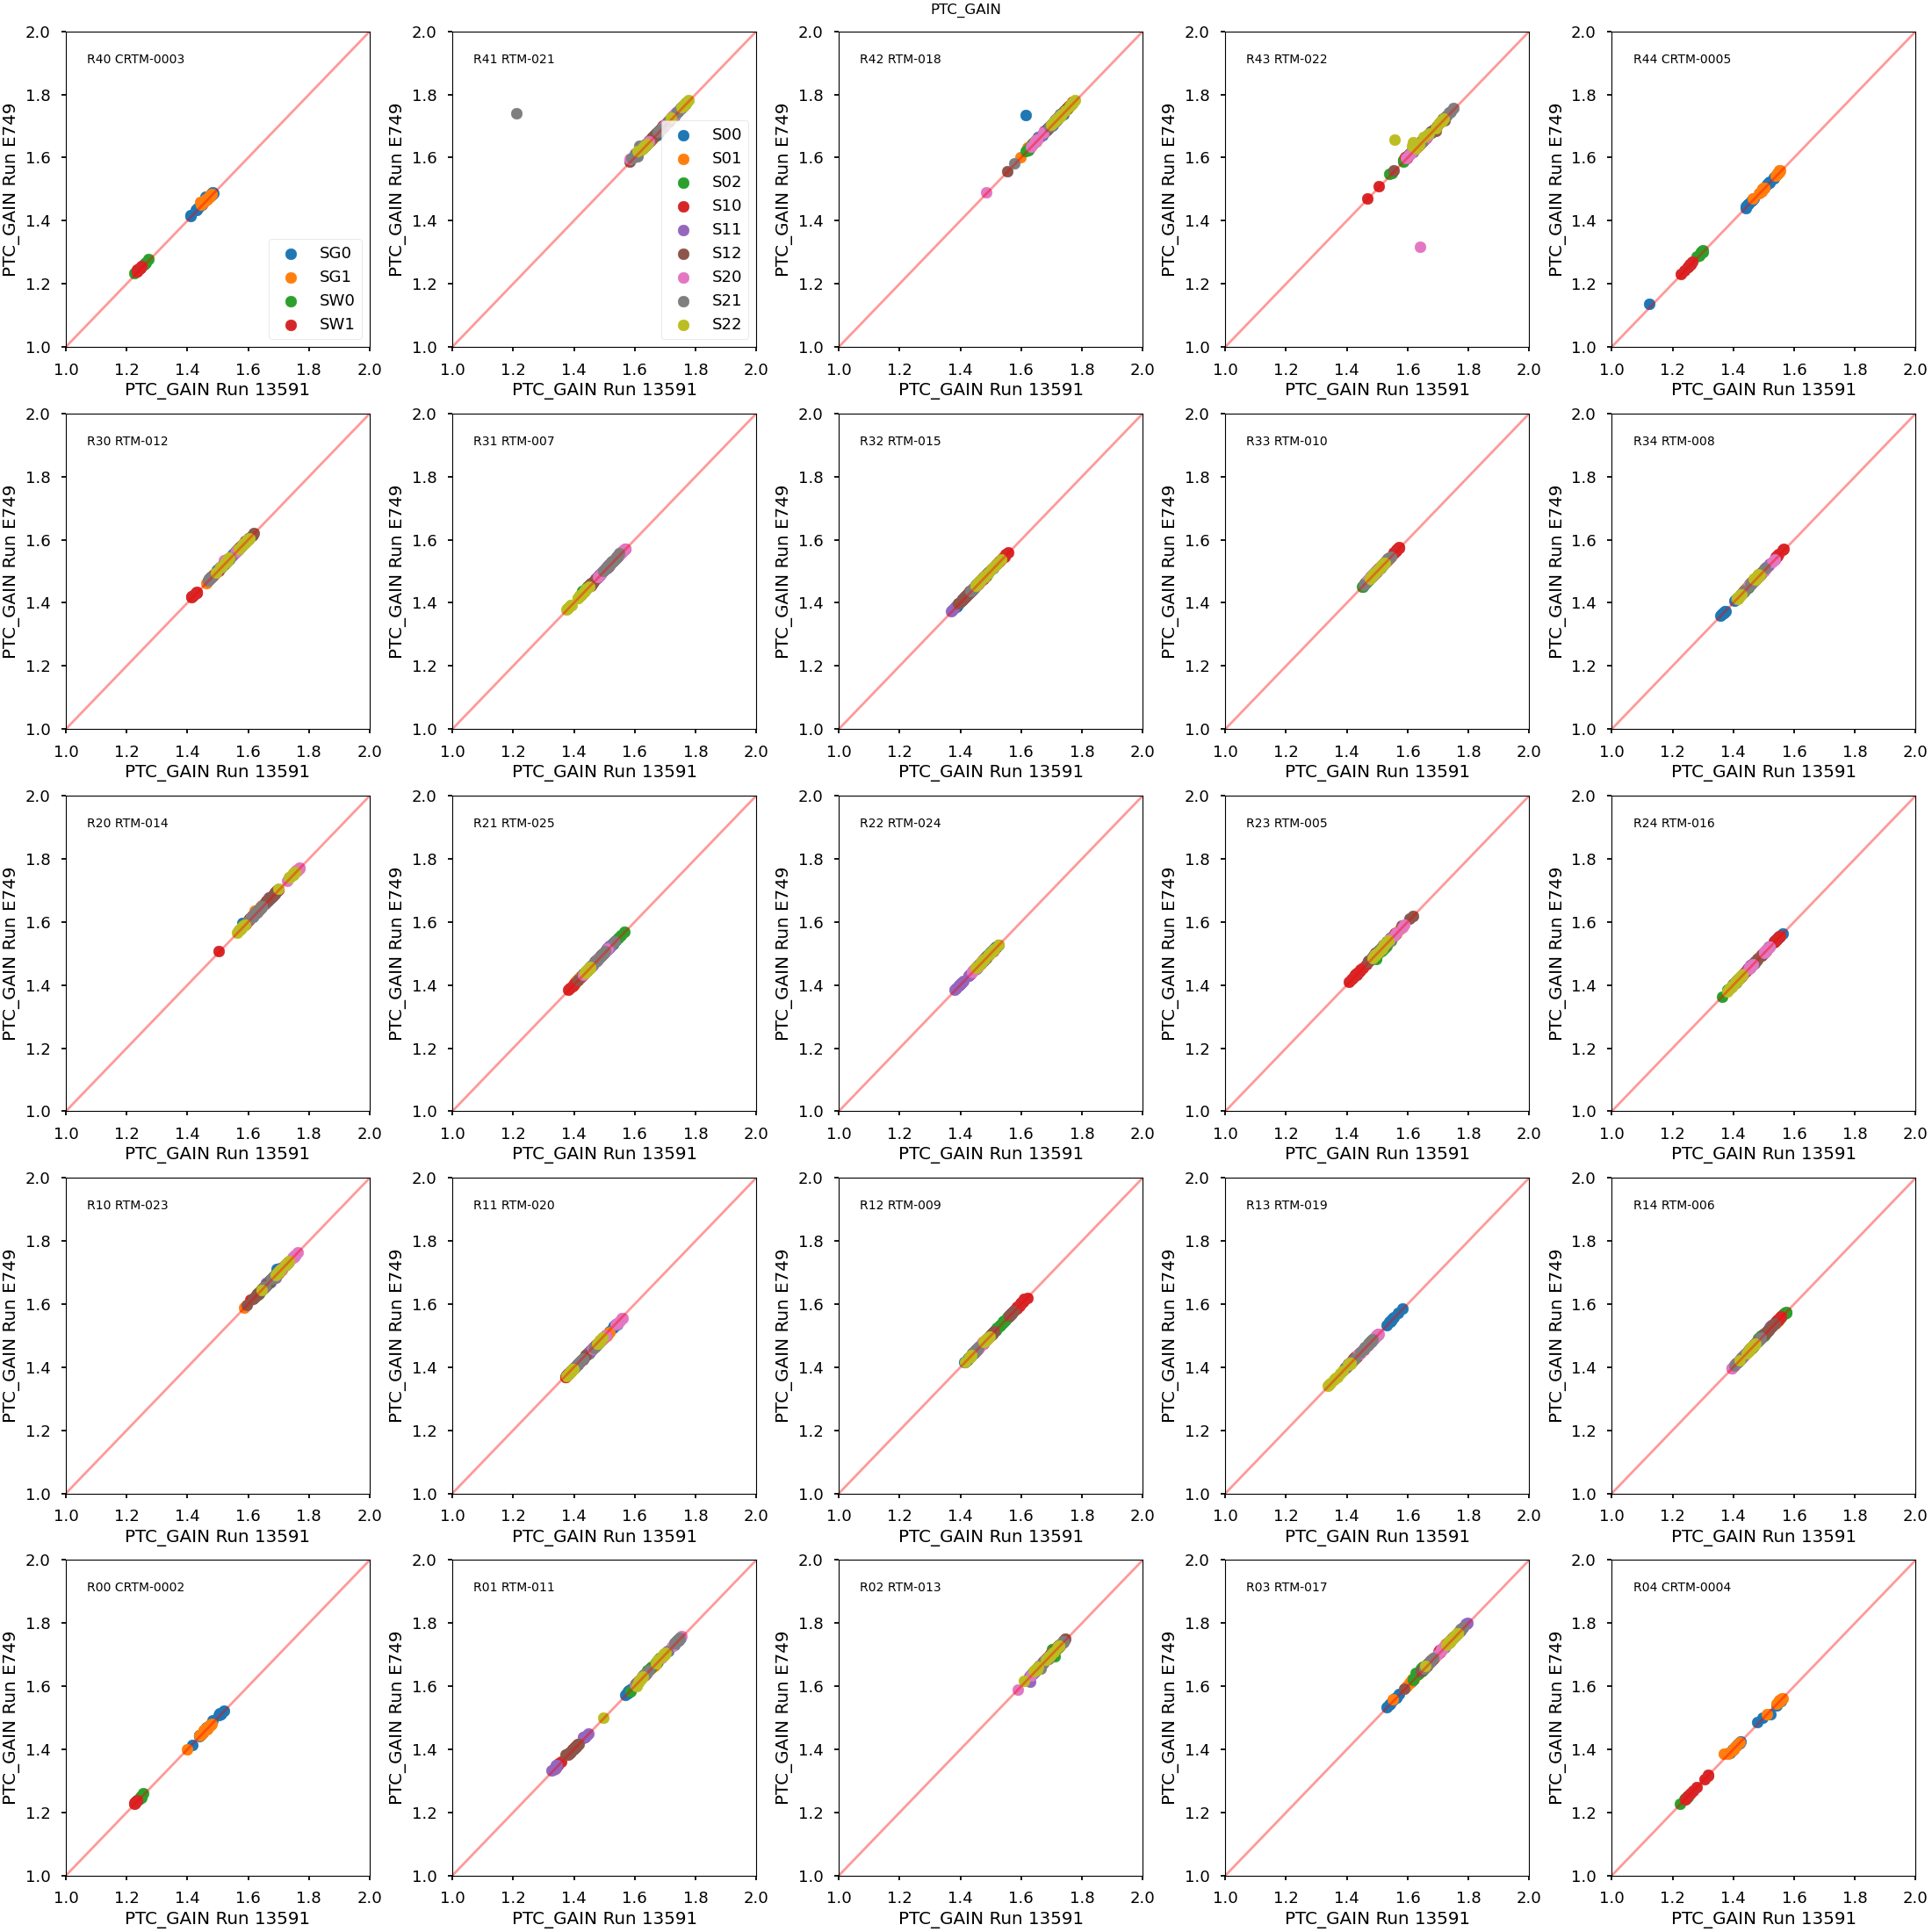
\includegraphics[width=0.7\textwidth]{figures/baselineCharacterization/13591_E749_PTC_GAIN.png}
\caption{A comparison of Run 6 and Run 7 amplifier measurements in gain, separated by sensor type. For both sensor types, gain is very consistent.}
\end{centering}
\end{figure}

PTC gain measurements agree extremely closely across all sensors in the
focal plane.

\clearpage

\subsubsection{Read Noise}\label{sec:initialRever:ReadNoise}

Read noise is induced charge during the readout process of the LSST Camera sensors. Common causes of read noise include thermal noise in the electronics or imperfect charge transfer. Read noise is measured in electrons, and is calculated by taking the standard deviation of the overscan region.

\begin{figure}[ht]
\begin{centering}
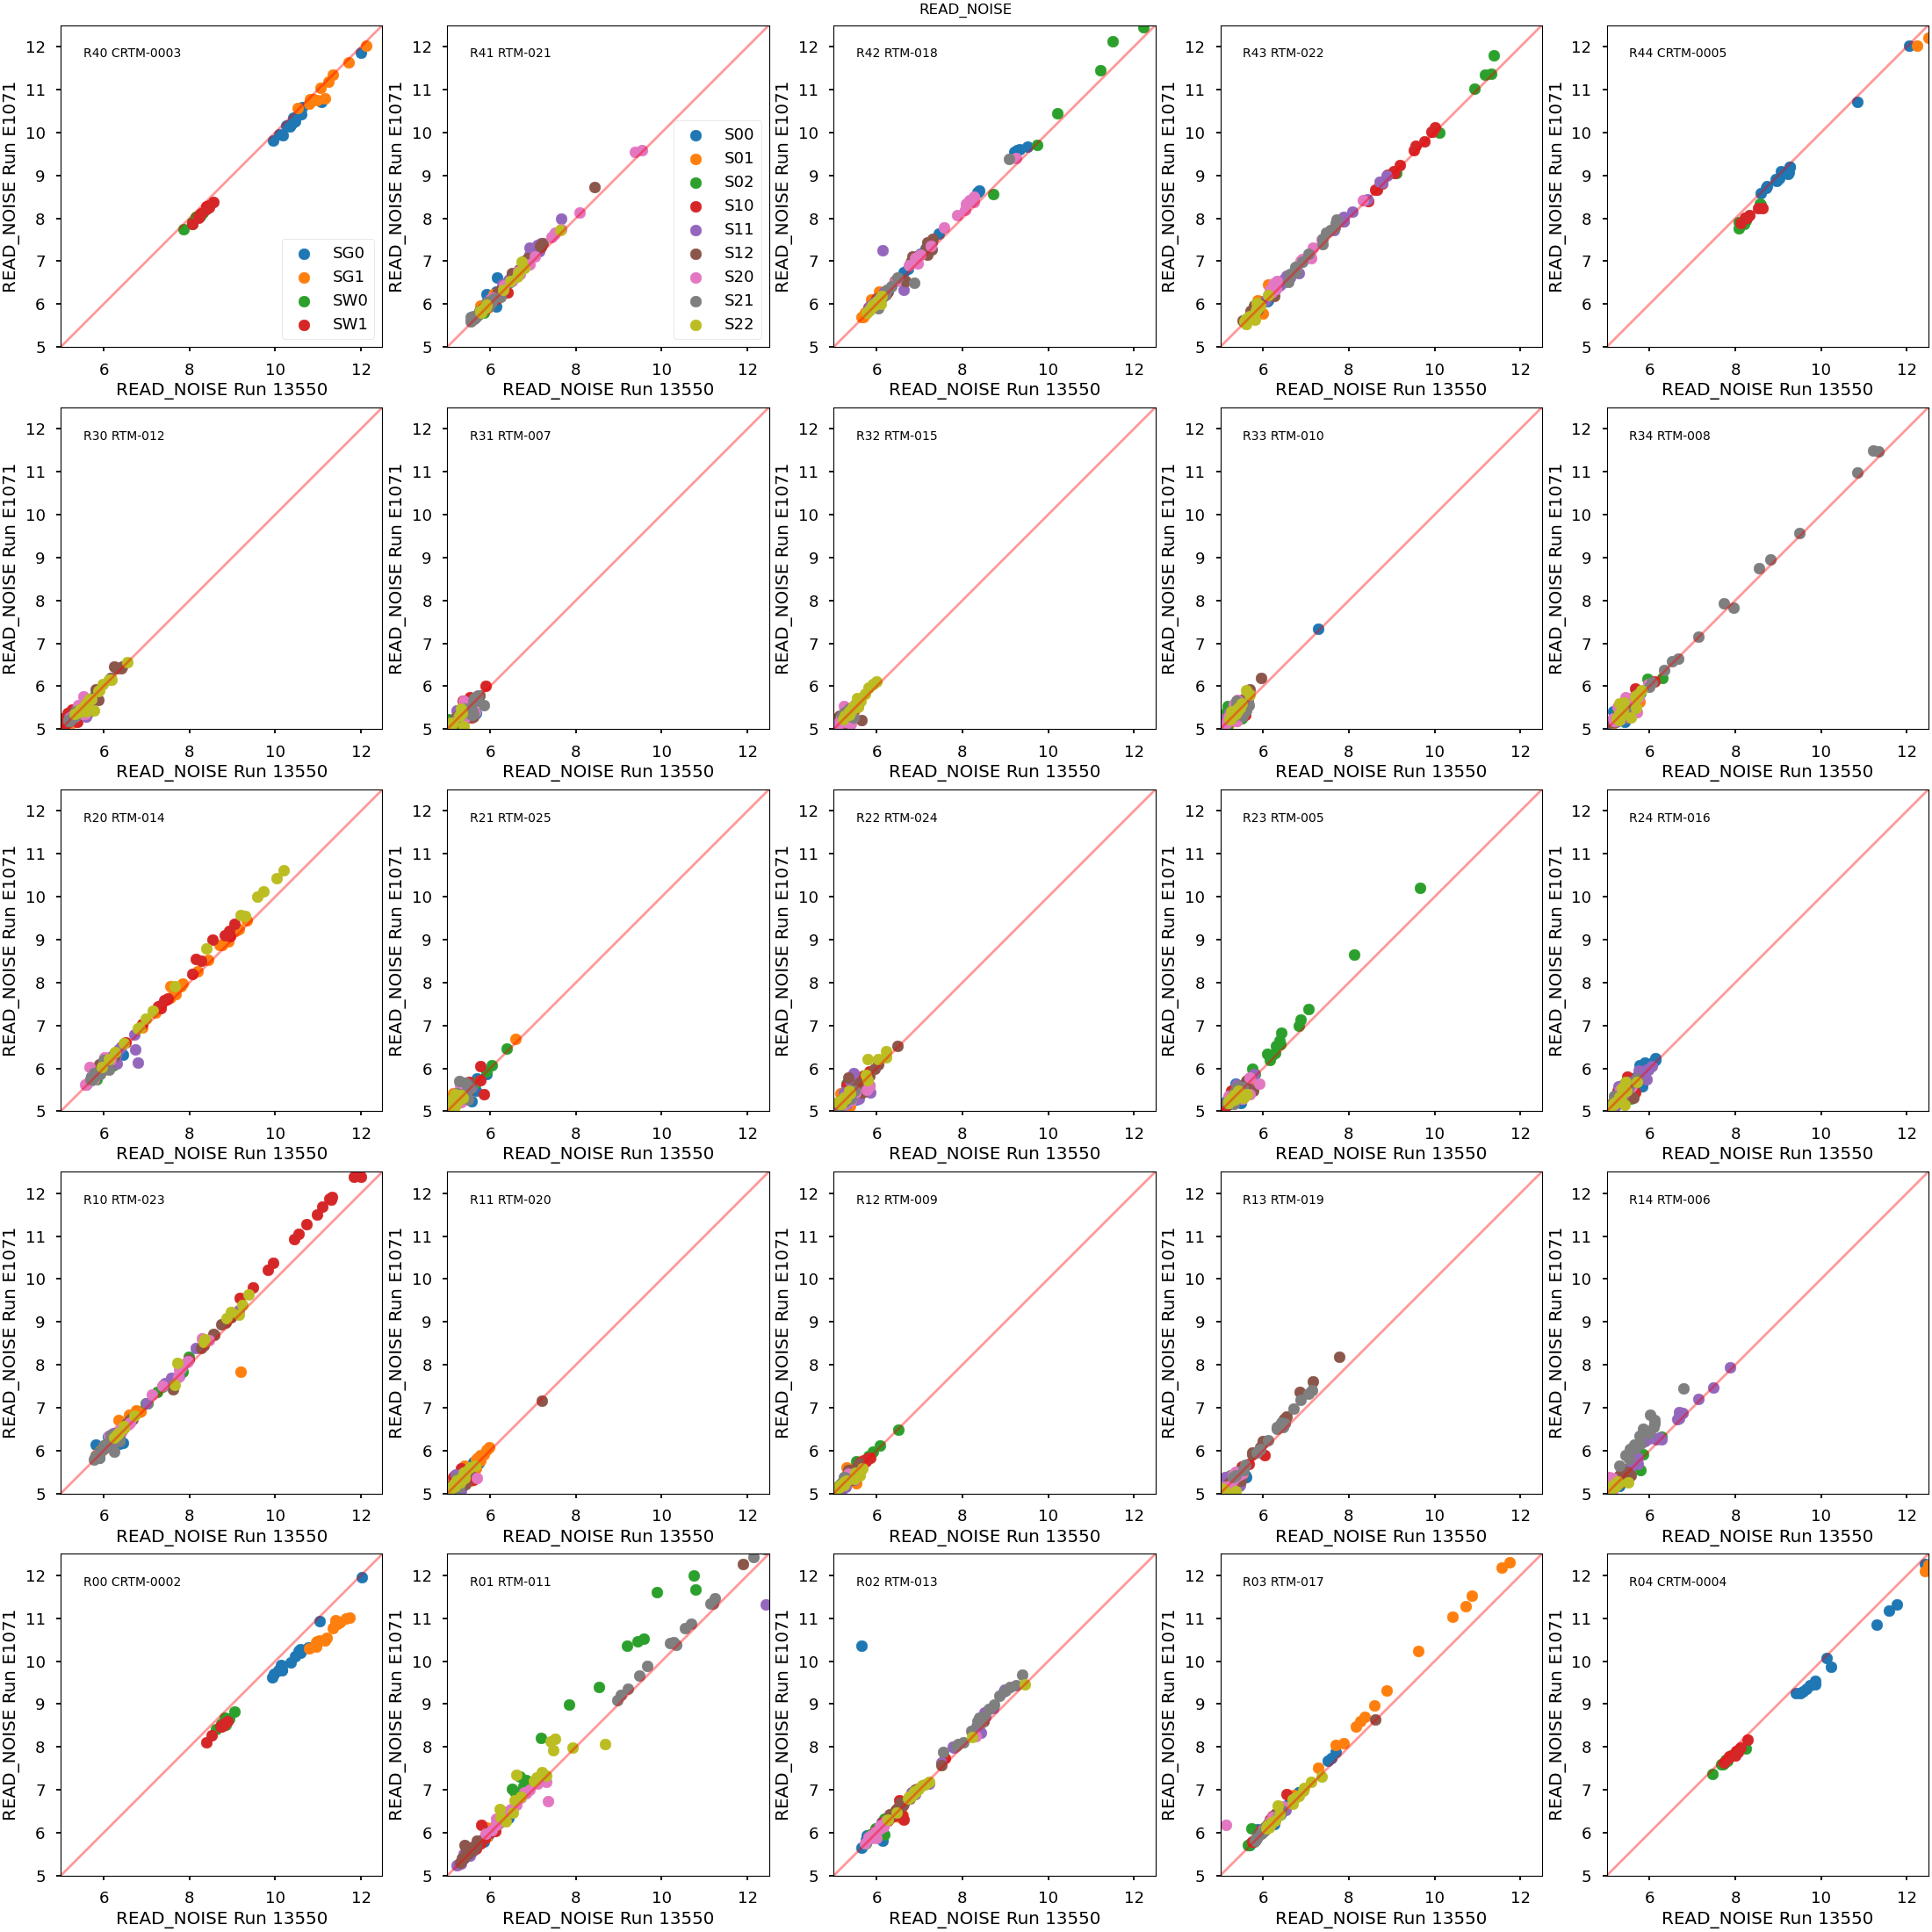
\includegraphics[width=0.7\textwidth]{figures/baselineCharacterization/13550_E1071_READ_NOISE_inset.png}
\caption{A comparison of Run 6 and Run 7 amplifier measurements for read noise, separated by sensor type. For both sensor types, read noise is higher in Run 7.}
\end{centering}
\end{figure}

The read noise is higher in Run 7 than Run 6 for both sensor types. The difference is on the order of 0.05 e-.

\begin{figure}[ht]
\begin{centering}
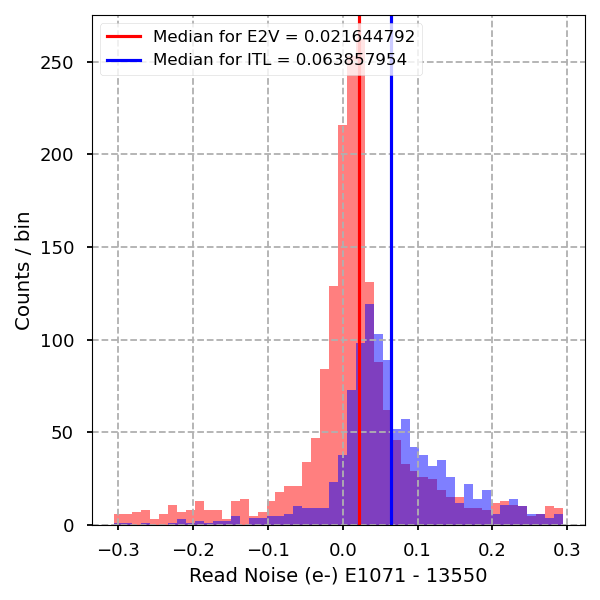
\includegraphics[width=0.7\textwidth]{figures/baselineCharacterization/ReadNoisee-_13550_E1071_diff.png}
\caption{A comparison of Run 6 and Run 7 amplifier measurements for read noise, separated by sensor type. For both sensor types, read noise is higher in Run 7.}
\end{centering}
\end{figure}

\subsubsection{PTC Noise}\label{sec:initialRever:PTCNoise}

PTC noise is a fitted parameter in the PTC model, and is the foundation of the PTC model. In the shot noise regime, where the PTC slope is 1/2 in log-log space (from 500 - 10k ADU in figure \ref{fig:initRever:PTC_Comparison}), the data can be fitted to a line. The intercept of that line is the PTC noise, measured in ADU.

\begin{figure}[ht]
    \centering
    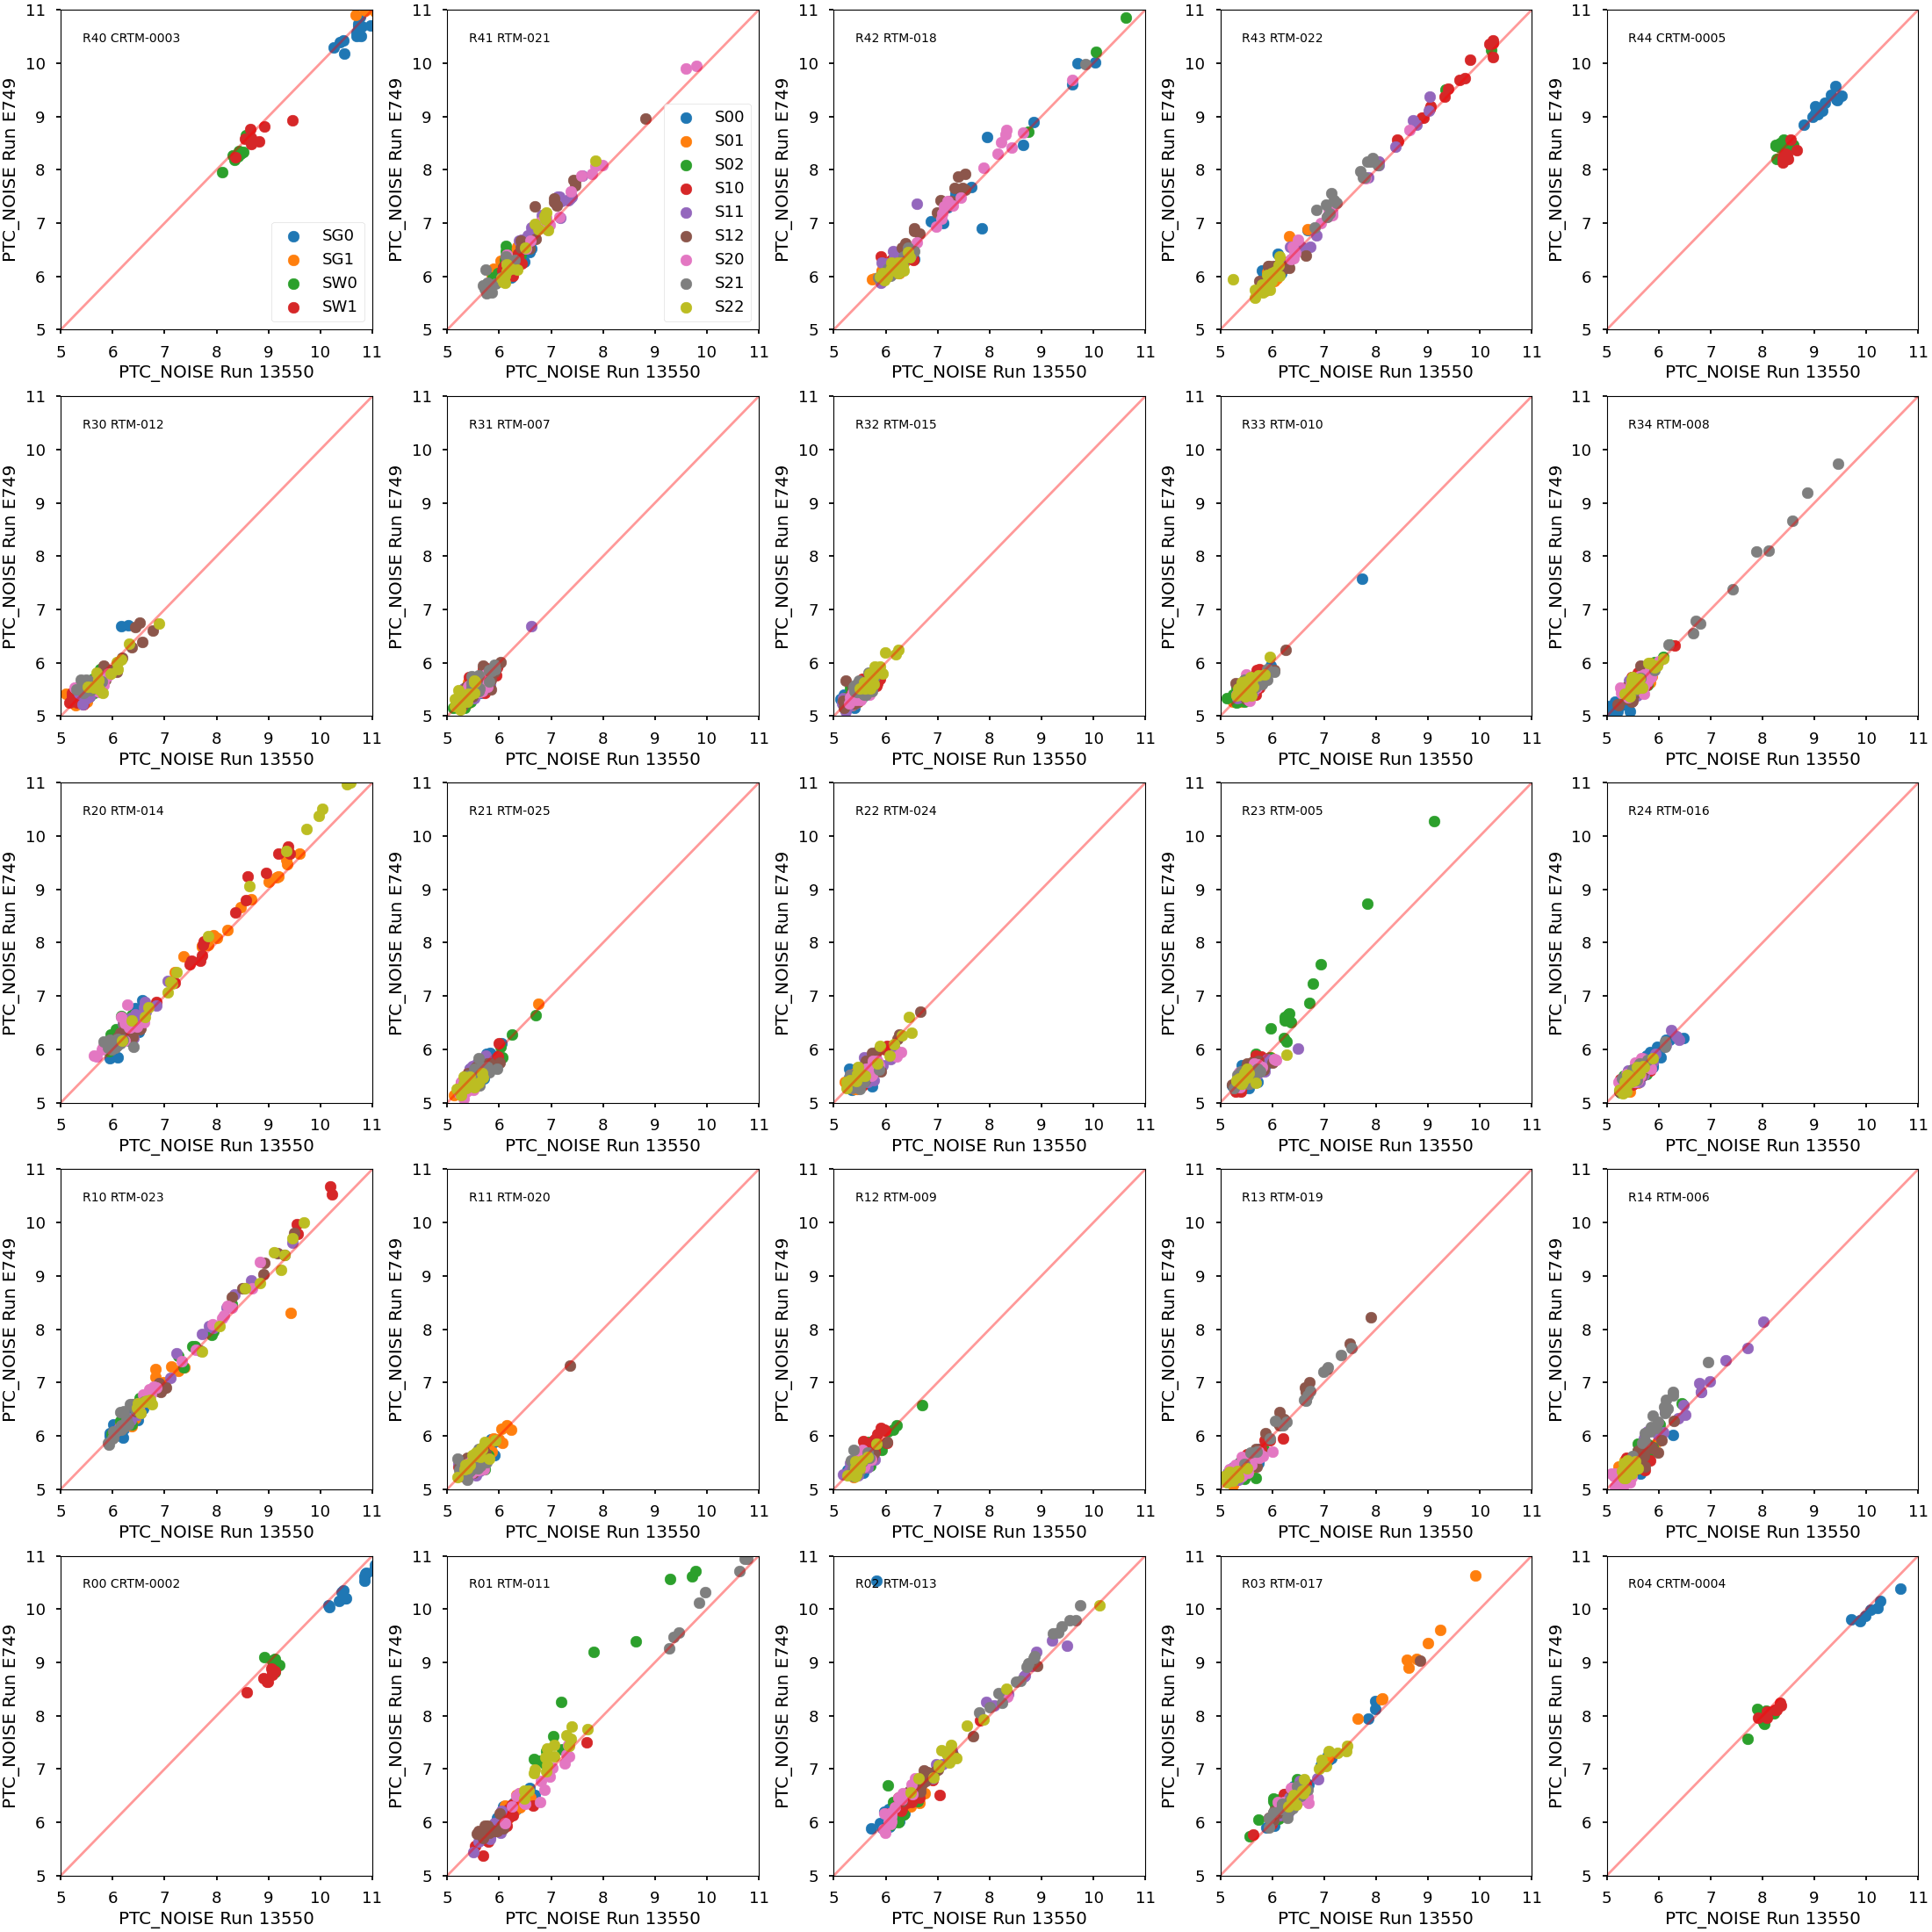
\includegraphics[width=0.7\linewidth]{figures/baselineCharacterization/13550_E749_PTC_NOISE.png}
    \caption{Comparison of amplifier measurements of PTC noise for initial and final Run 7 conditions.}
    \label{fig:initRever-PTC_NOISE_5x5}
\end{figure}

PTC noise differs by $\lesssim$ 0.1 e- on average for science sensors. Notably, e2v sensors measure a PTC noise 0.02 e- lower in Run 7, while ITL sensors measure a PTC noise 0.08 e- higher in Run 7 (see figure \ref{fig:initRever:PTCNoise_hist_diff}).

\begin{figure}[ht]
    \centering
    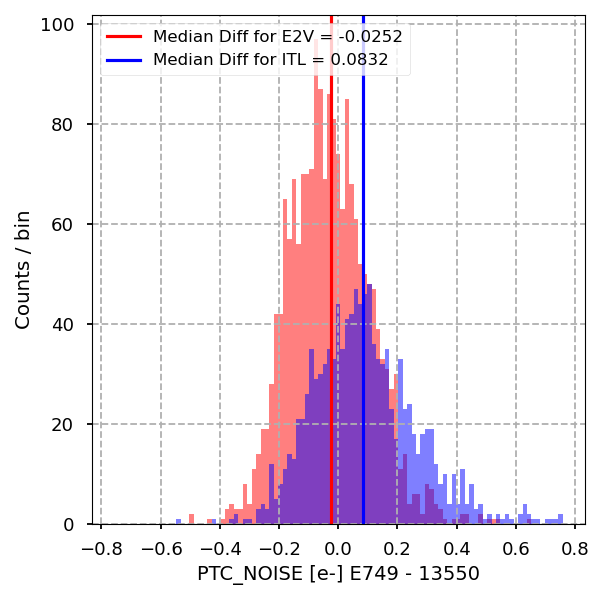
\includegraphics[width=0.7\linewidth]{figures/baselineCharacterization/PTC_NOISE_13550_E749_diff.png}
    \caption{Comparison of the PTC noise measurements in different sensors and run types.}
    \label{fig:initRever:PTCNoise_hist_diff}
\end{figure}


\subsubsection{Brighter-fatter coefficients}\label{brighter-fatter-a00-coefficient}


The brighter-fatter effect in CCDs refers to the phenomenon where brighter sources appear larger (or ``fatter" than dimmer ones). This occurs due to electrostatic interactions within the pixel wells of the CCDs, when a pixel accumulates a high charge from incoming photons and creates an electric field that slightly repels incoming charge carriers into neighboring pixels. The brighter-fatter effect can be modeled as the most dominant source of pixel-pixel correlations. Following the PTC model from  
\citet{2019A&A...629A..36A}, $a_{00}$ describes the change of a pixel area due to its own charge content, or the relative strength of the brighter-fatter effect. Since same-charge carriers repel each other, the pixel area decreases as charge accumulates inside the pixel well, which implies $a_{00}$ \textless{} 0. Similarly $a_{10}$ describes the area change cause by a pixel to its nearest serial neighbor, and $a_{01}$ to the parallel nearest neighbor. Figs. \ref{fig:hist_as_run6_7} and \ref{fig:ratio_bf_coeff_6_7} compare the measurement of these coefficients carried out at SLAC and at the summit. We see that the variations are modest (and could be explained by noise) except for two rafts: R10 and R11. The Run 6 data used for this comparison was acquired with a high voltage of 45V applied to these two rafts, rather than the usual 50\,V. The sensitivity of our measurements of the brighter-fatter coefficients is sufficient to detect the change of electrostatic conditions due to this change of drift field in the sensors. In {\tt eo\_pipe}, an absolute value is taken of the $a_{00}$ parameter, so the tabulated quantities are positive.

\begin{figure}[ht]
    \begin{centering}
  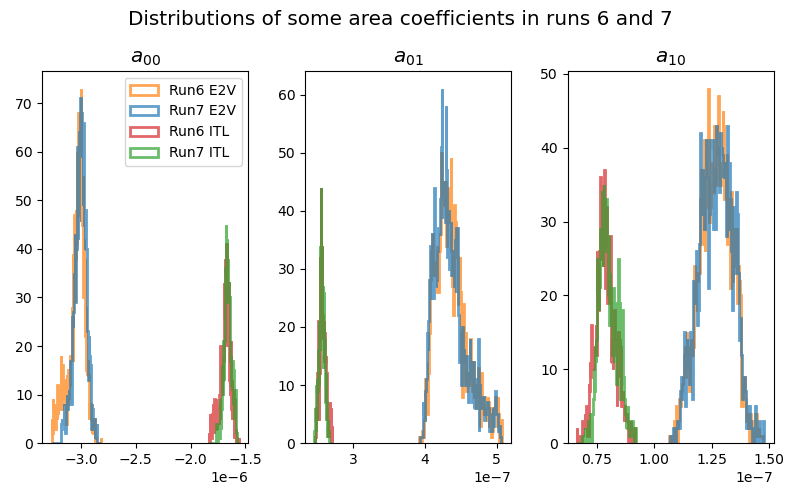
\includegraphics[width=0.7\linewidth]{figures/hist_as_run6_7.png}

  \caption{Distributions of $a_{00}$, $a_{01}$ and $a_{10}$ in Run 6 and Run 7. Those are very similar, except for two rafts, which had a lower drift electric field (45\,V vs. 50\,V) in Run 6. The ratios are displayed in Figure~\ref{fig:ratio_bf_coeff_6_7}.\label{fig:hist_as_run6_7}}
  \end{centering}
  \end{figure}

\begin{figure}[ht]
  \begin{centering}
   \minipage{0.32\textwidth}
  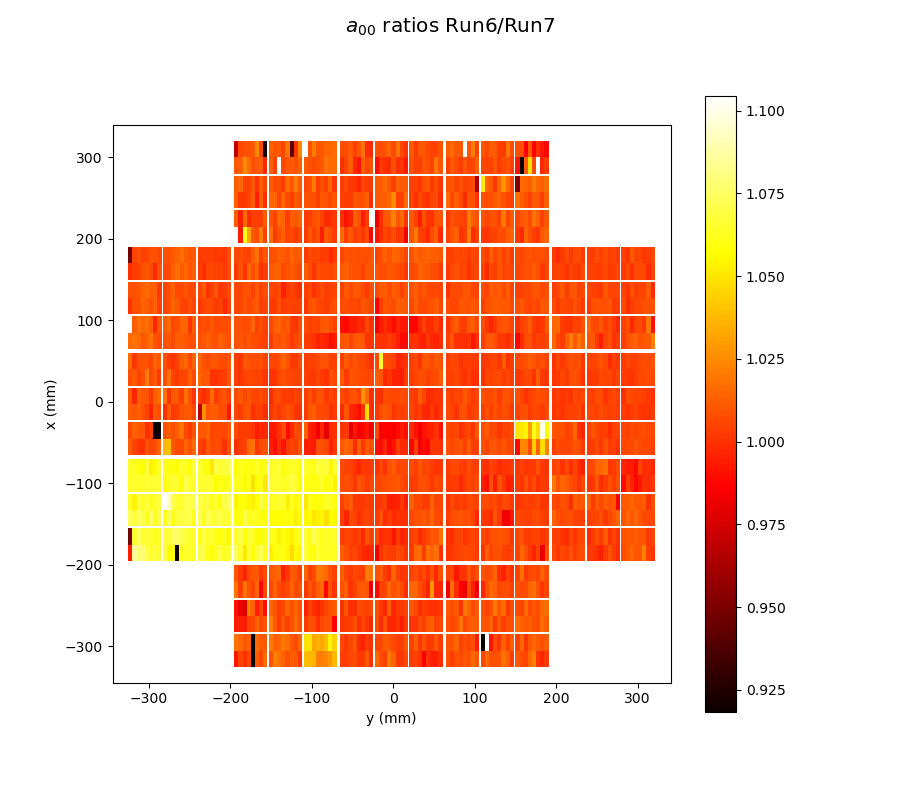
\includegraphics[width=\linewidth]{figures/baselineCharacterization/a00_ratios.png}
  \endminipage\hfill
   \minipage{0.32\textwidth}
  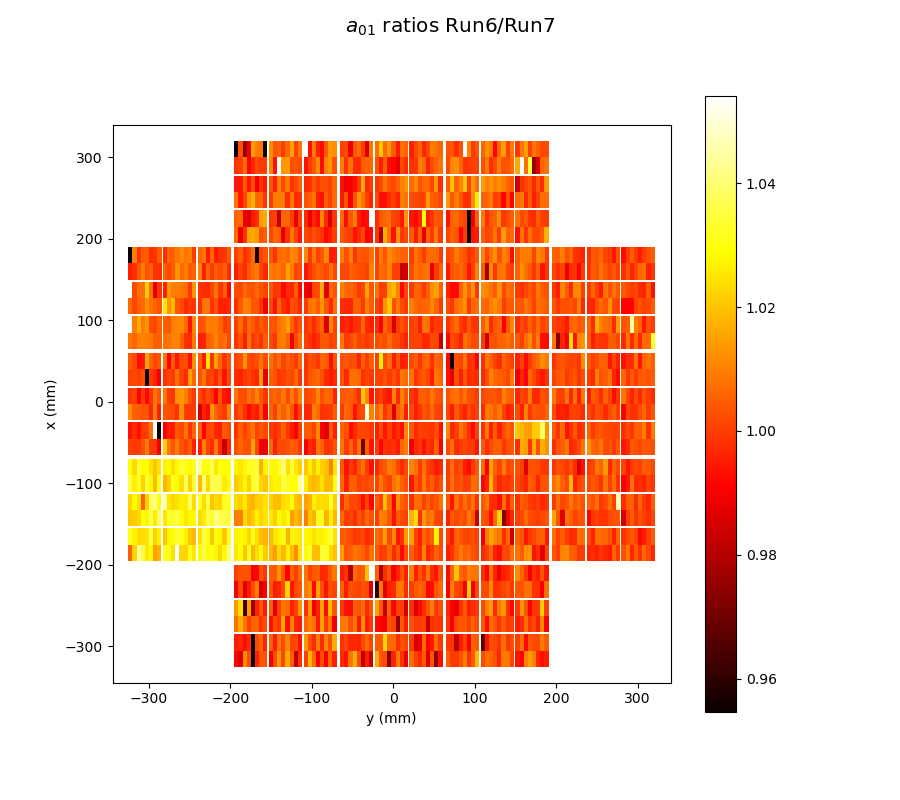
\includegraphics[width=\linewidth]{figures/baselineCharacterization/a01_ratios.png}
  \endminipage\hfill
   \minipage{0.32\textwidth}
  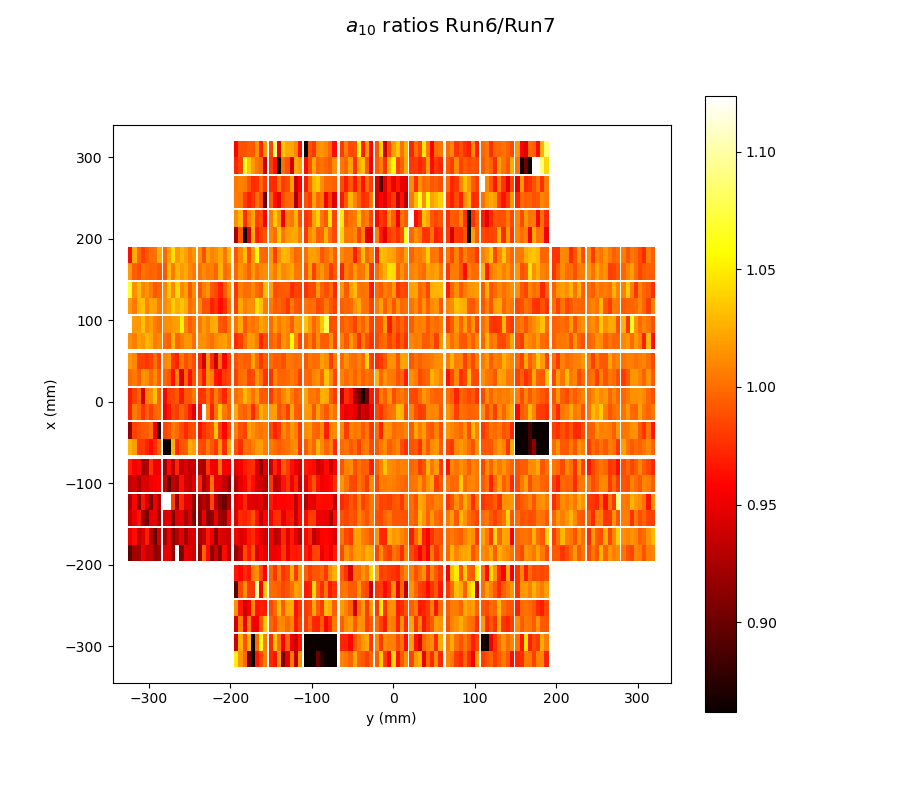
\includegraphics[width=\linewidth]{figures/baselineCharacterization/a10_ratios.png}
  \endminipage\hfill
  

\caption{Ratio of measurements of $a_{00}$, $a_{01}$ and $a_{10}$ coefficients (one per amplifier) for Run 6 and Run 7. They are very consistent, except for two rafts (R10 and R11) where the high voltage was changed between the two runs.\label{fig:ratio_bf_coeff_6_7}}
  \end{centering}
  \end{figure}

The distribution of the difference of $a_{00}$ measurements between the runs is displayed in Figures~\ref{fig:ptc_a00_diff_hist} and \ref{fig:ptc_a00_5x5}.

\begin{figure}[ht]
\begin{centering}
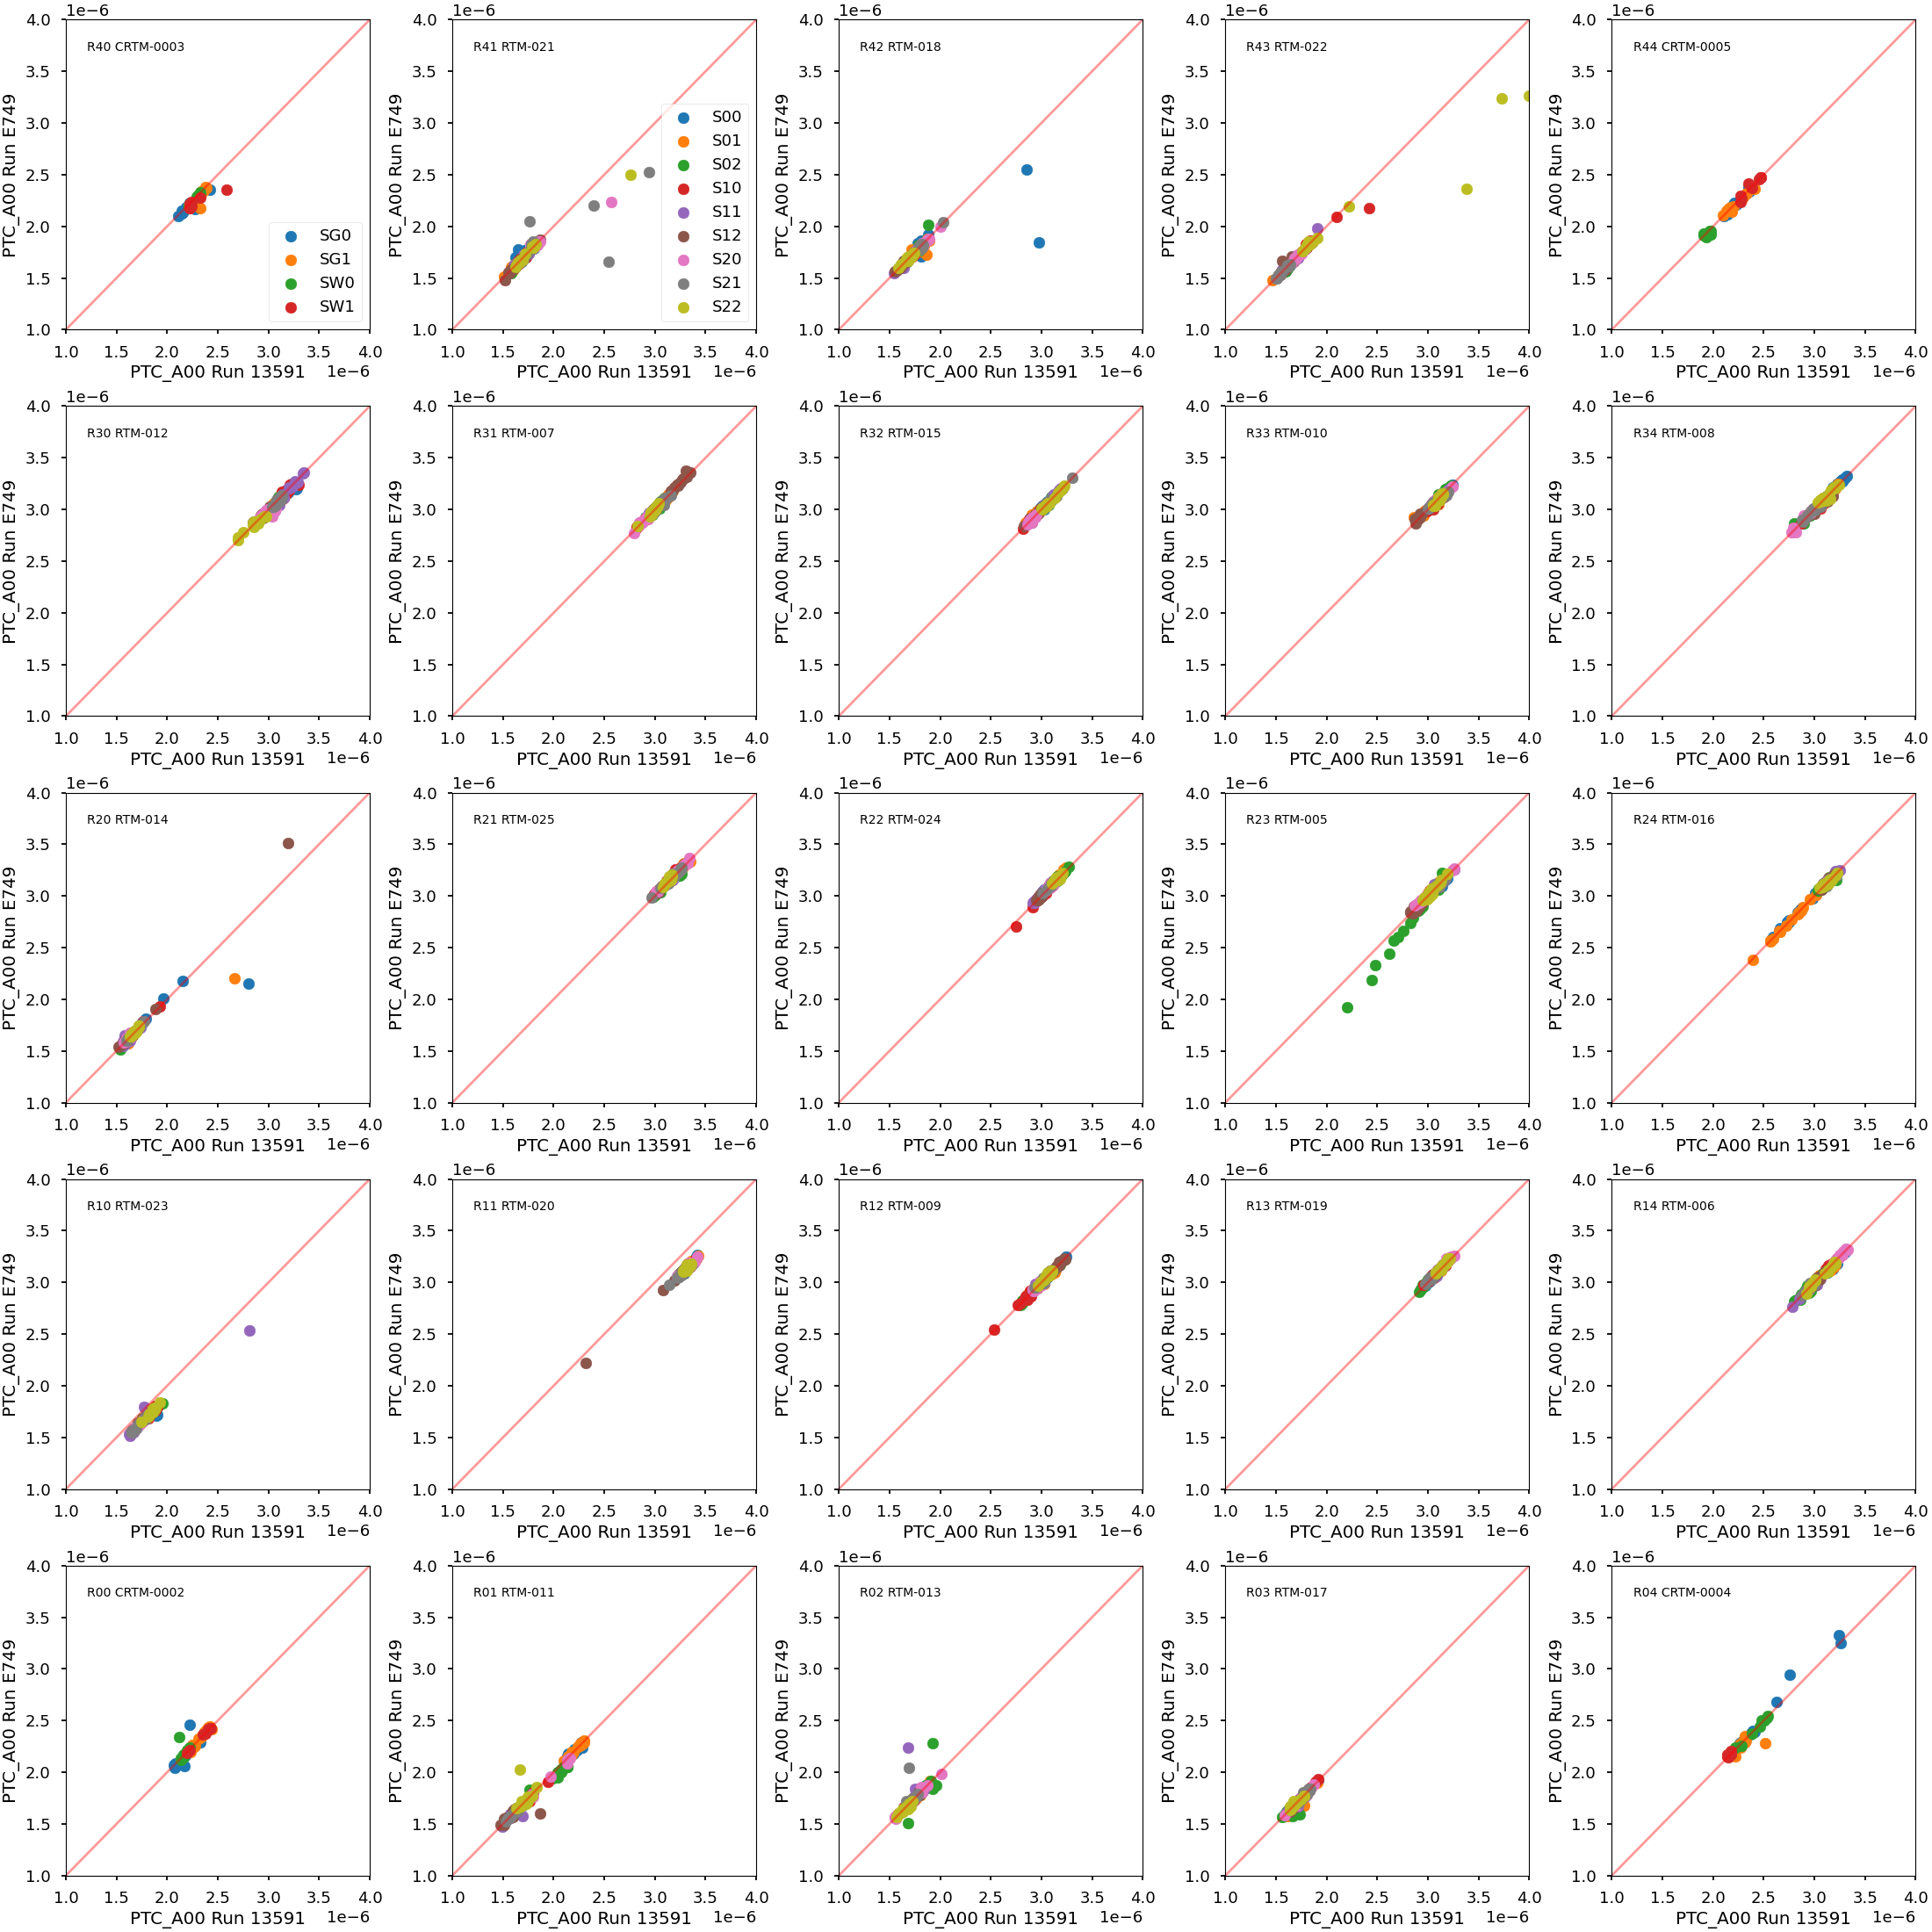
\includegraphics[width=0.7\textwidth]{figures/baselineCharacterization/13591_E749_PTC_A00.png}
\caption{Comparison of Run 6 and Run 7 amplifier differences in the $a_{00}$ coefficient, separated by amplifier across the focal plane. The amplifiers associated with R10 and R11 are noted outliers, as seen in figure \ref{fig:ratio_bf_coeff_6_7}.}
\label{fig:ptc_a00_5x5}
\end{centering}
\end{figure}

\begin{figure}[ht]
\begin{centering}
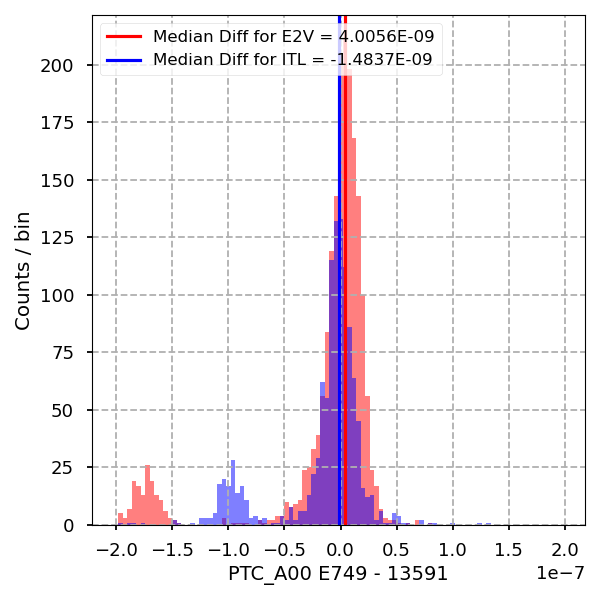
\includegraphics[width=0.7\textwidth]{figures/baselineCharacterization/PTC_A00_13591_E749_diff.png}
\caption{A comparison of Run 6 and Run 7 amplifier differences in the $a_{00}$ coefficient, separated by sensor type. For both sensor types, the $a_{00}$ coefficient is very consistent. The two peaks on the left represent the two outlier rafts visible on Figure \ref{fig:ratio_bf_coeff_6_7}. The $a_{00}$ values are of the order of 2 to 3 $10^{-6}\ e^{-1}$. \label{fig:ptc_a00_diff_hist}}
\end{centering}
\end{figure}

However, the differences in the brighter-fatter $a_{00}$ coefficient between Run 6 and Run 7 show that the magnitude of $a_{00}$ decreased for most of the outliers, which implies an improvement in imaging for those pixels.

\clearpage
\subsubsection{Row-means variance}\label{row-means-var}

Row-means variance is a metric that measures the mean row-to-row variance of differences between a pair of flats. By computing variance of means of differenced rows at each flux level, we can measure any changes in gain row-by-row and also changes in correlated noise along with row.

\begin{figure}[ht]
\begin{centering}
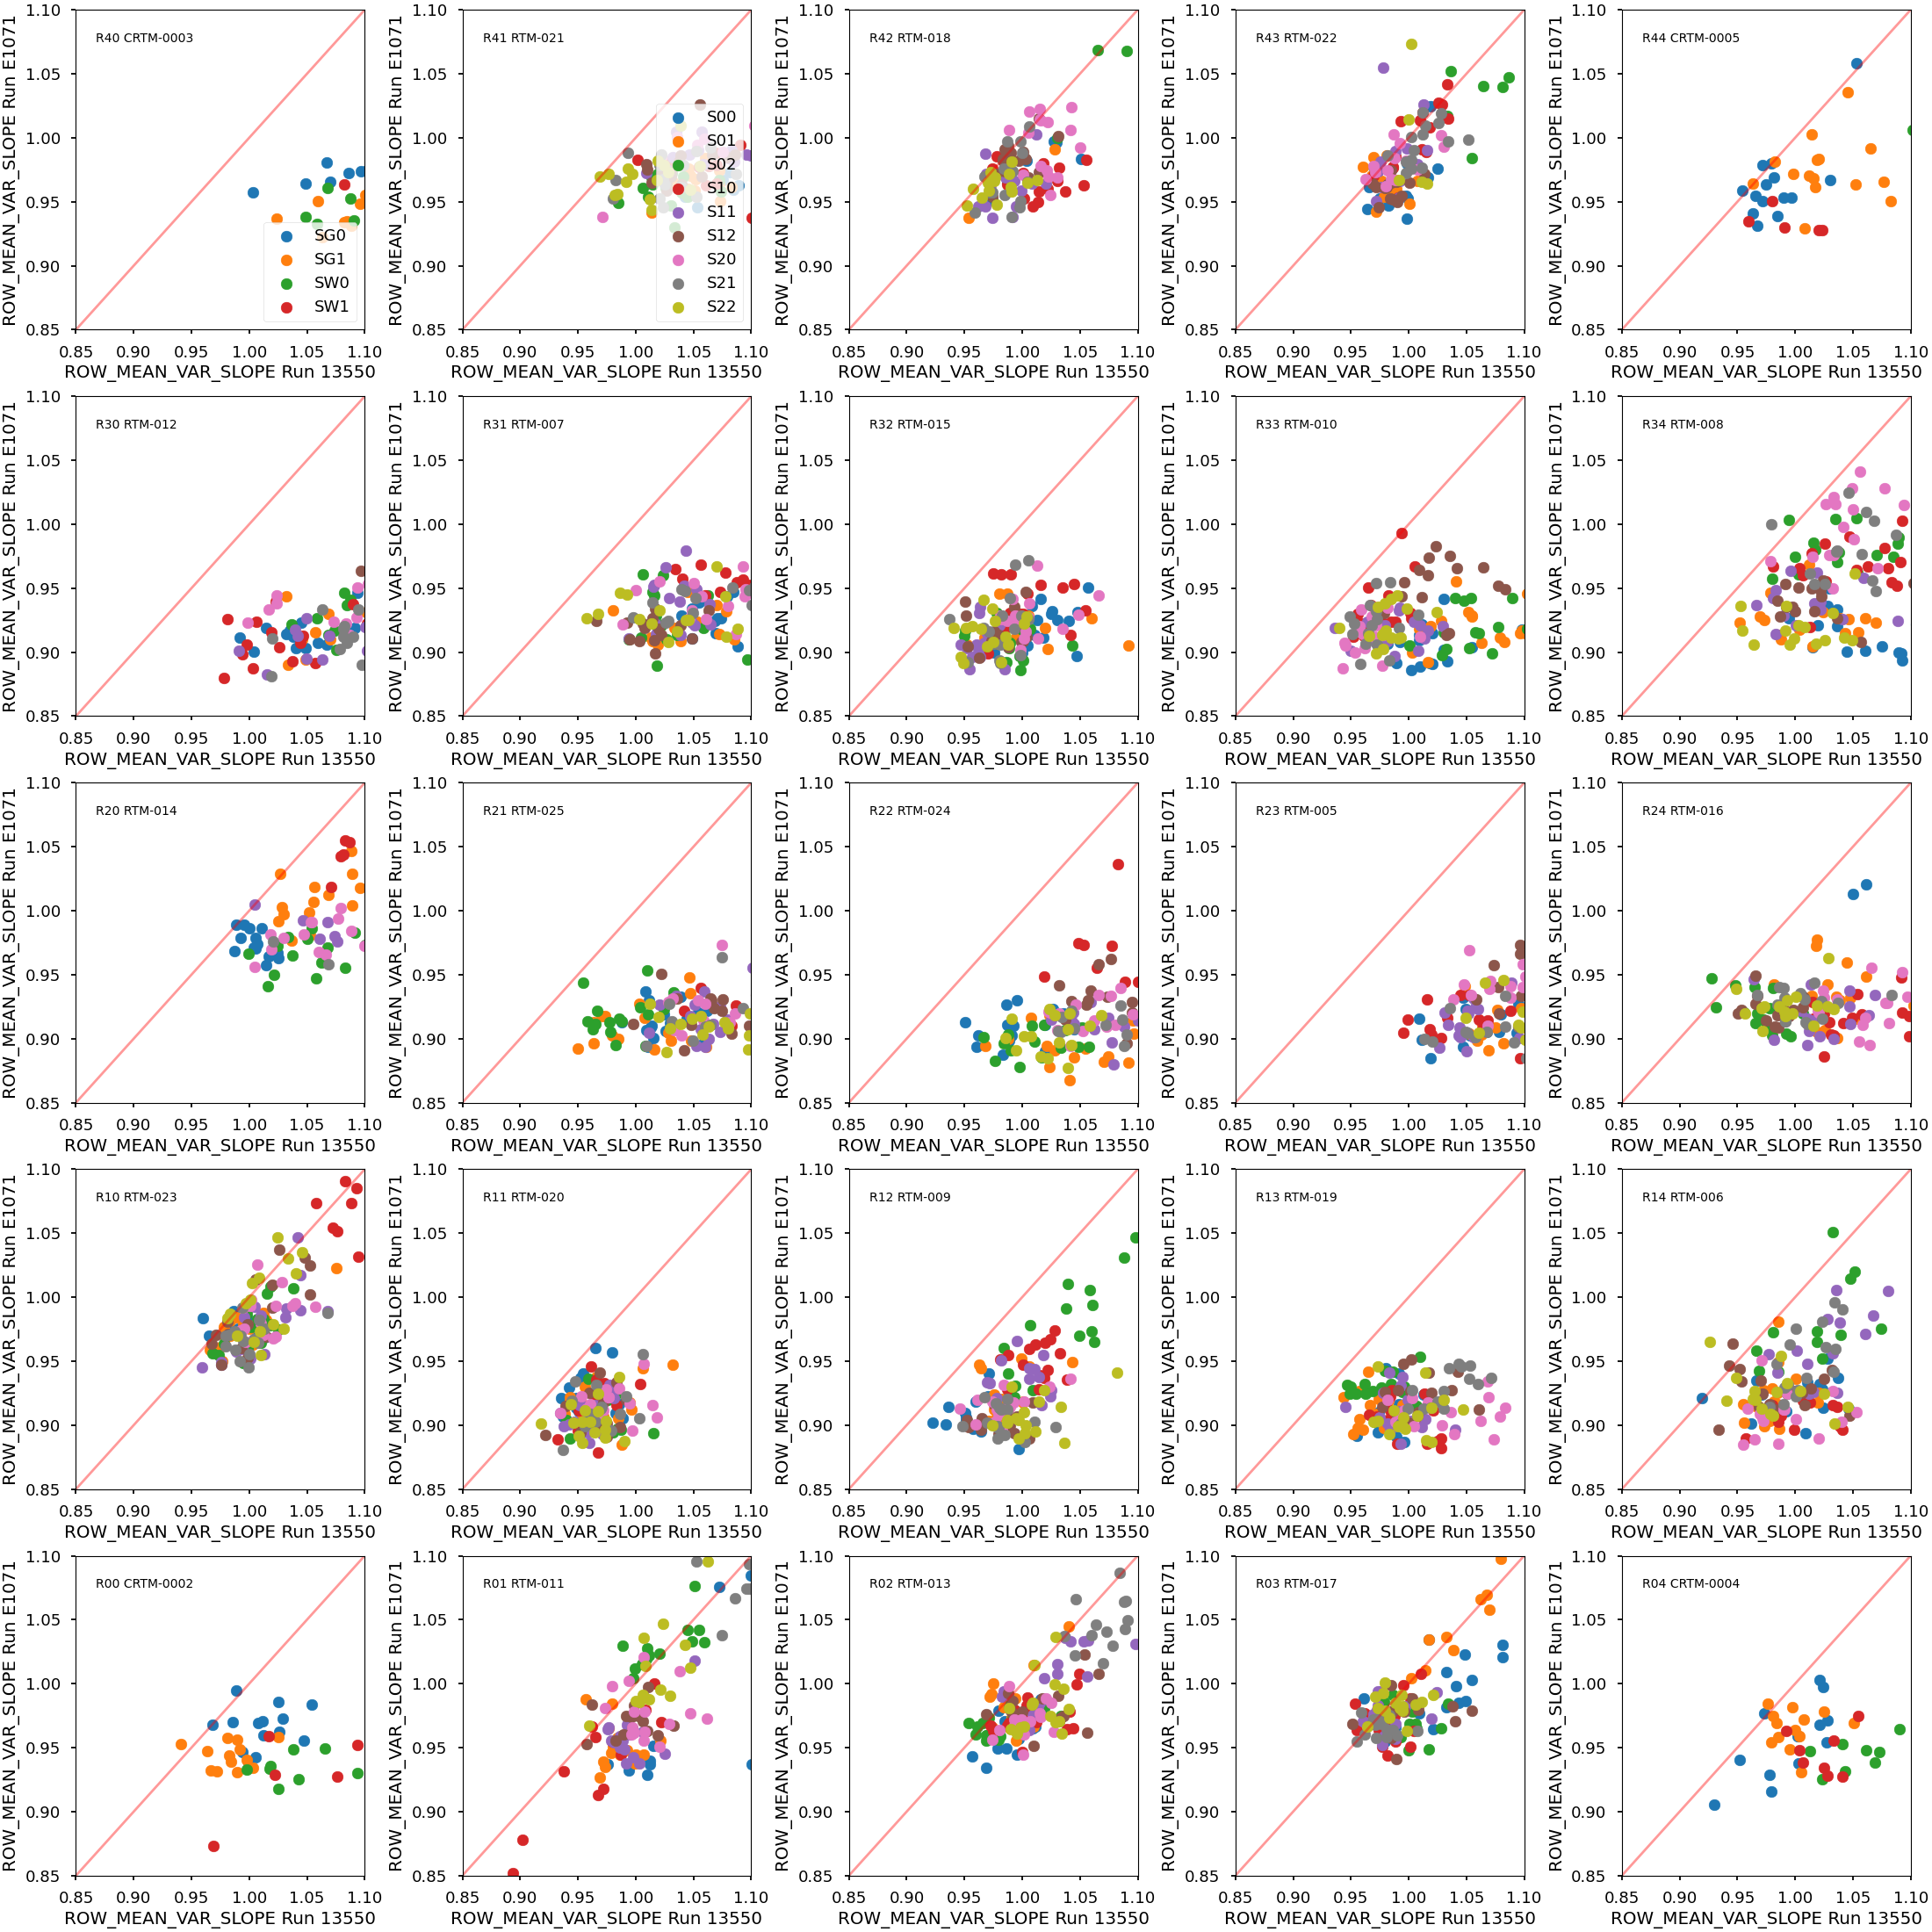
\includegraphics[width=0.7\textwidth]{figures/baselineCharacterization/13550_E1071_ROW_MEAN_VAR_SLOPE.png}
\caption{A comparison of Run 6 and Run 7 amplifier differences in row-mean-variance slope. For both sensor types, row-means-variance slope is weaker in Run 7. This is more pronounced for e2v sensors.}
\end{centering}
\end{figure}

Differences in row-means variance between runs are evident, and are distinctly different for different detector types. The difference between runs is more significant for ITL sensors, \textasciitilde9\% smaller on average in Run 7. For e2v sensors, the effect is \textasciitilde3\% smaller in Run 7. This indicates that either row-by-row correlated noise or row-by-row gain change is less in Run 6. Since we did not change the sequencer file, the most natural explanation is the row-by-row correlated noise. But further investigation is needed.

\begin{figure}[ht]
\begin{centering}
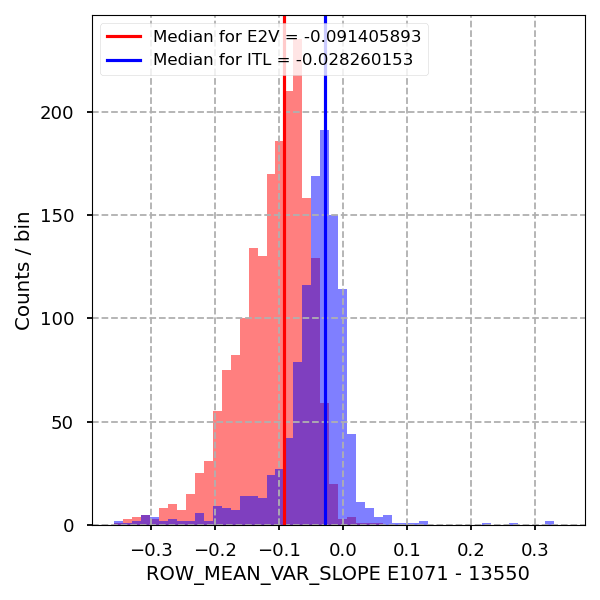
\includegraphics[width=0.7\textwidth]{figures/baselineCharacterization/ROW_MEAN_VAR_SLOPE_13550_E1071_diff.png}
\caption{A comparison of Run 6 and Run 7 amplifier differences in row-mean-variance slope, separated by sensor type. For both sensor types, row-means-variance slope is weaker in Run 7. This is more pronounced for e2v sensors.}
\end{centering}
\end{figure}

\clearpage
\subsubsection{Divisadero tearing}\label{sec:divisadero:init}

Divisadero tearing (or Rabbit ears) manifests as signal variations near amplifier boundaries, connected features that are often jagged \cite{2020arXiv200209439J,2024SPIE13103E..0WU}. These variations are on the order of \textasciitilde1\% relative to the flat field signal. To quantify divisadero tearing in a given column, we measure the column signal, and compare it to the mean column signal from flat fields.

\begin{figure}[ht]
\begin{centering}
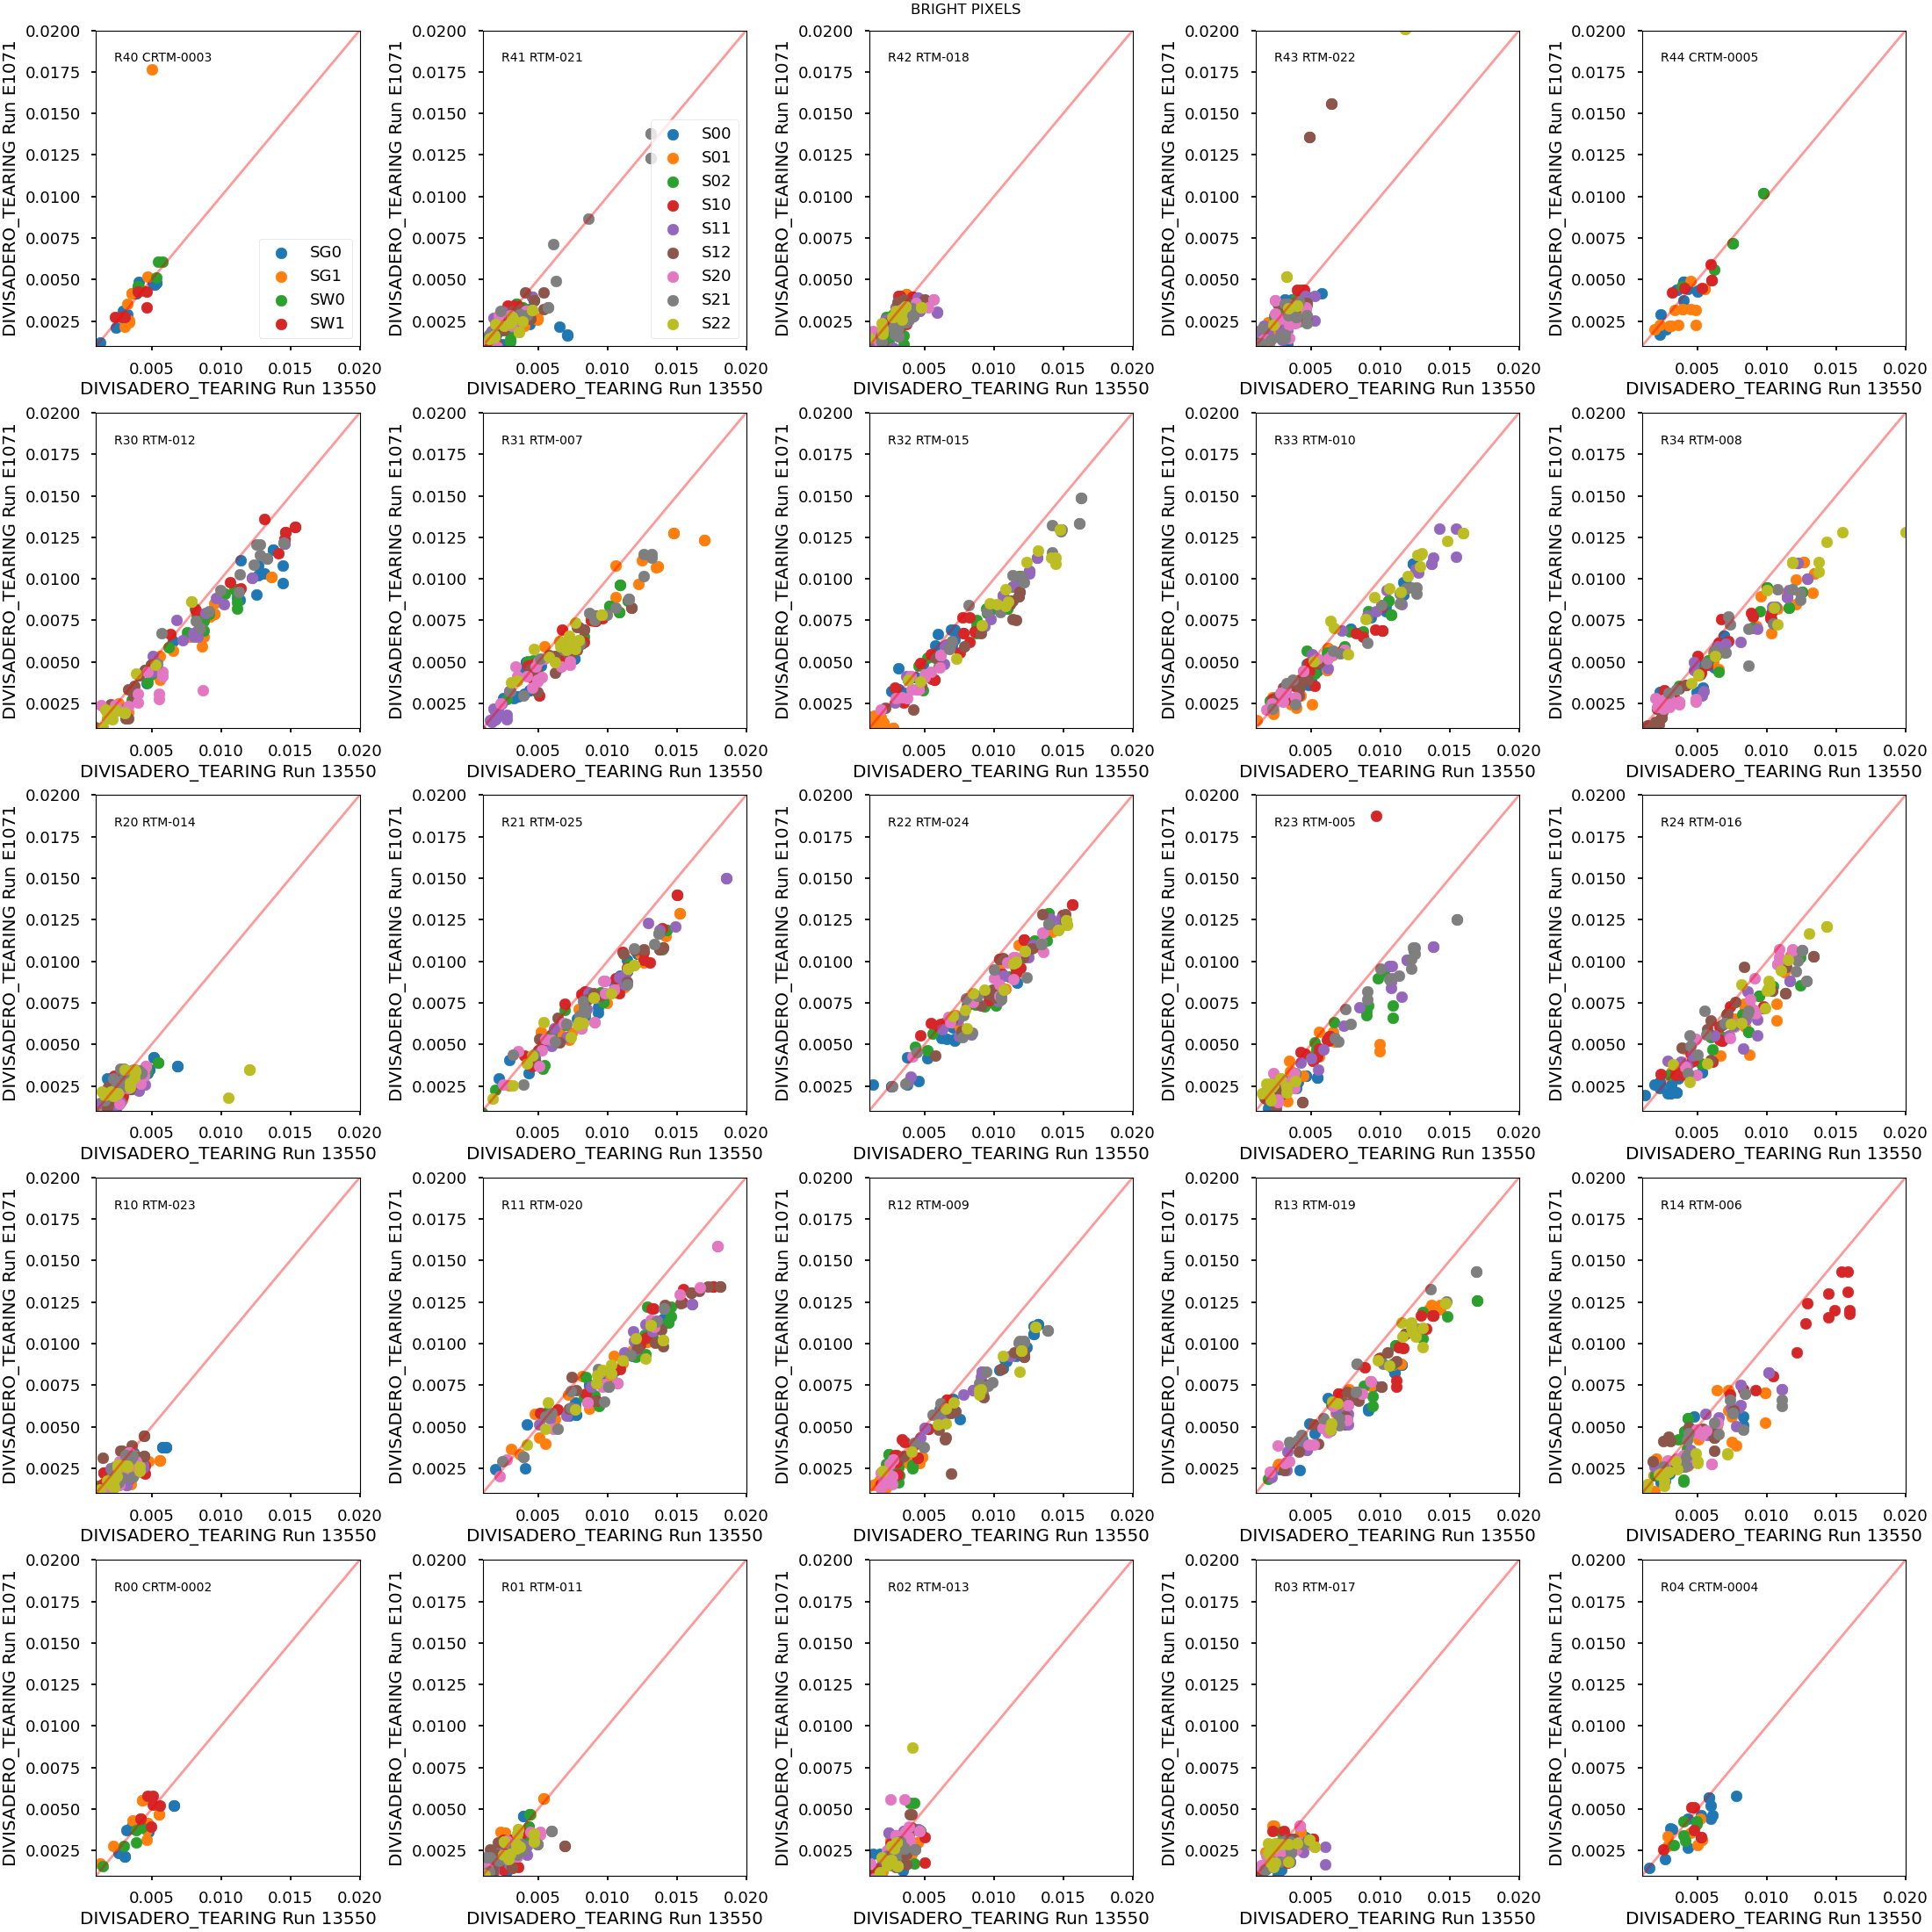
\includegraphics[width=0.7\textwidth]{figures/baselineCharacterization/13550_E1071_DIVISADERO_TEARING_inset.png}
\caption{A comparison of Run 6 and Run 7 amplifier differences in Divisadero tearing, separated by sensor type. For both sensor types, divisadero tearing is weaker in Run 7. The difference is more pronounced for e2v sensors, which have larger divisadero tearing in general.}
\end{centering}
\end{figure}

Divisadero tearing is broadly consistent between Run 6 and Run 7, with both sensor types demonstrating lower divisadero tearing in Run 7. Taking amplifier differences, e2v sensors show a weaker divisadero signal in Run 7 by 0.1\%, while ITL sensors demonstrate a weaker Divisadero signal in Run 7 by 0.05\% (see Fig.~\ref{fig:divisadero_diff_baseline}).

\begin{figure}[ht]
    \centering
    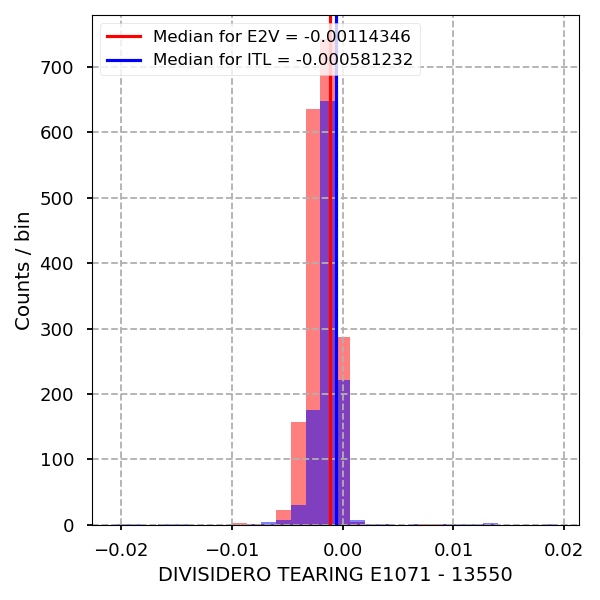
\includegraphics[width=0.7\linewidth]{figures/baselineCharacterization/DIVISIDERO_TEARING_13550_E1071_diff.png}
    \caption{Comparison of Run 6 and Run 7 amplifier differences in divisadero tearing, separated by sensor type. For both sensor types, divisadero tearing is weaker in Run 7.}
    \label{fig:divisadero_diff_baseline}
\end{figure}

\clearpage
\subsubsection{Dark defects}\label{dark-defects}

Dark defects are localized regions or individual pixels that produce abnormally low signal levels, even in the presence of light. Similarly to bright pixels, dark pixels are also quantified in dark columns over 50 pixel contiguous regions. These
defects are caused by imperfections in the semiconductor
material, imperfections during the manufacturing process of a CCD. For our evaluation, we extract dark pixels from combined flats, with the threshold for a dark defect defined as a $-$20\% deficit from the average flat field flux measured in the image segment.

\begin{figure}[ht]
\begin{centering}
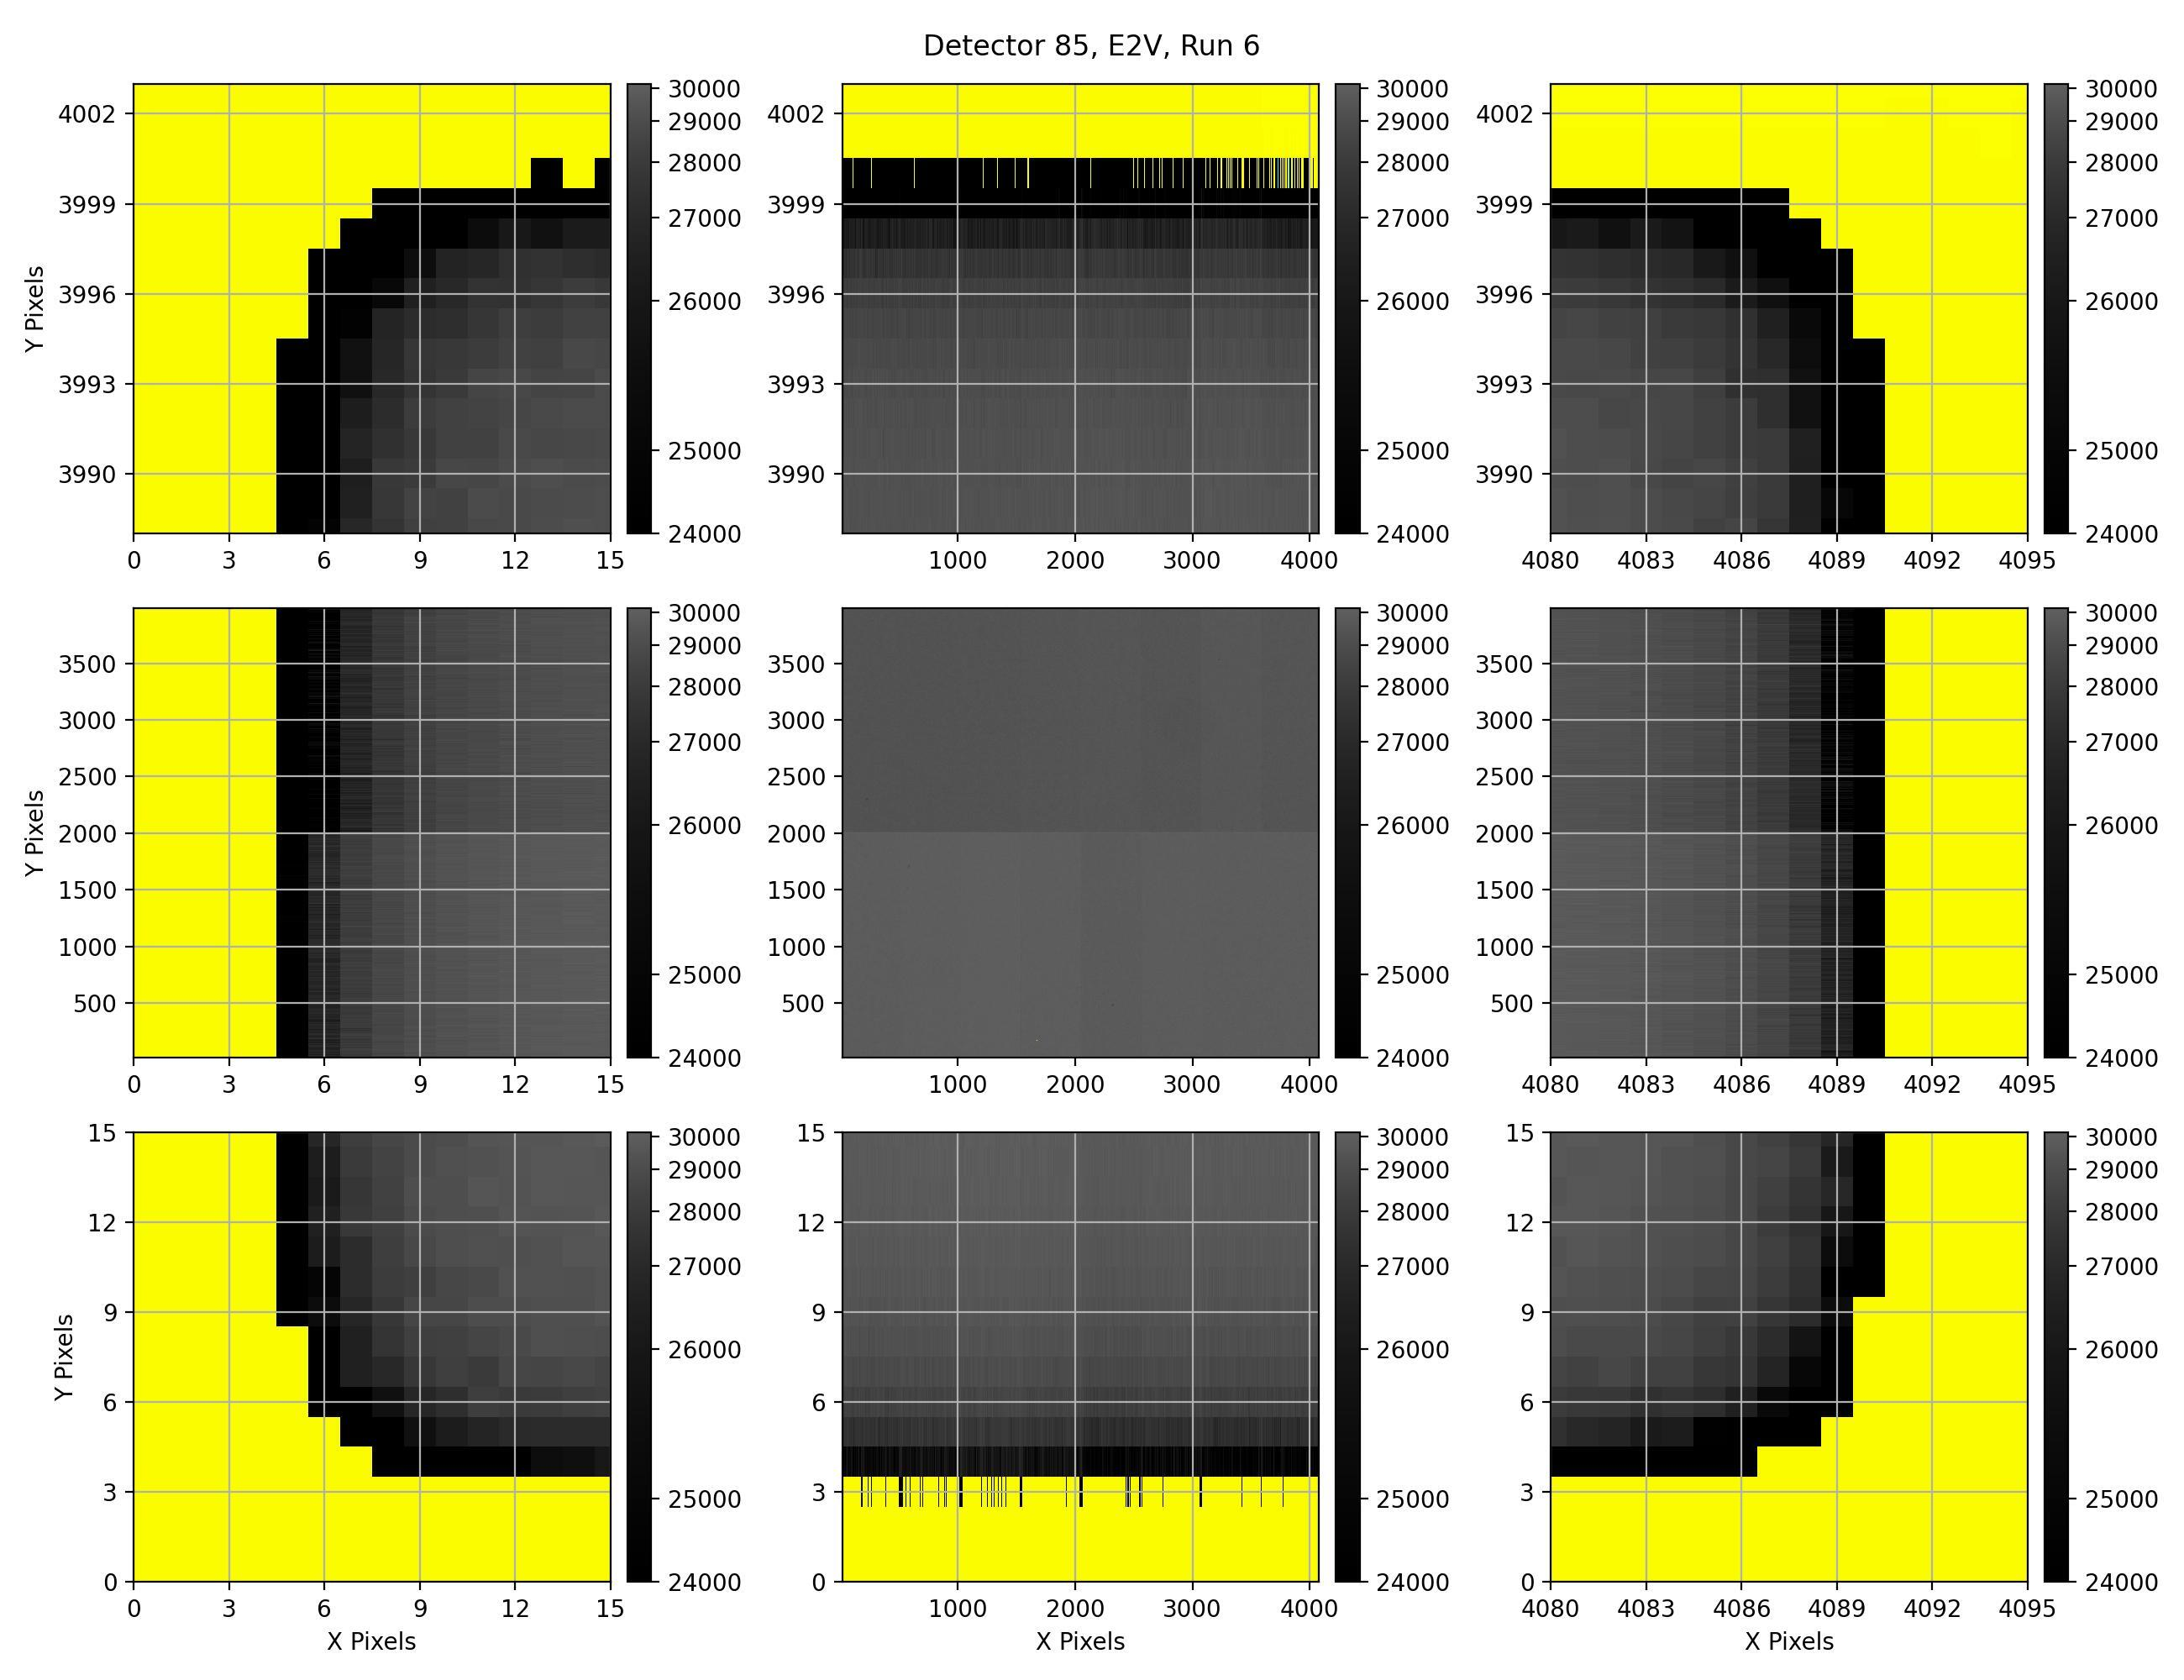
\includegraphics[width=0.7\textwidth]{figures/baselineCharacterization/detector_85.jpg}
\caption{Illustration of masked border pixels (yellow) for detector 85 (R21\_S11). The average defect mask size is 4 pixels along the serial (x-pixel) direction, and 5 pixels along the parallel direction. Additional dark defects exist in the sensor, but are difficult to quantify due to the overwhelming contribution from the picture frame response.}
\label{fig:fig-edge-mask}
\end{centering}
\end{figure}

%%
The eo-pipe configuration for evaluating dark defects considers a border pixel region that is masked differently from the dark pixels. The default size for this edge is zero pixels. With a zero pixel border mask, the average dark defect count is 1800 per amplifier, with \geq 95\% of the contribution coming from the picture frame. The `picture-frame response' (also called `edge roll-off') near the edges of the sensors is due to a decrease in the pixel active area. It is difficult to extract useful information about the dark defects in the focal plane without excluding the picture frame. The effects of the picture frame signal on dark defect masking is shown in figure~\ref{fig:fig-edge-mask}.


\begin{figure}[ht]
\begin{centering}
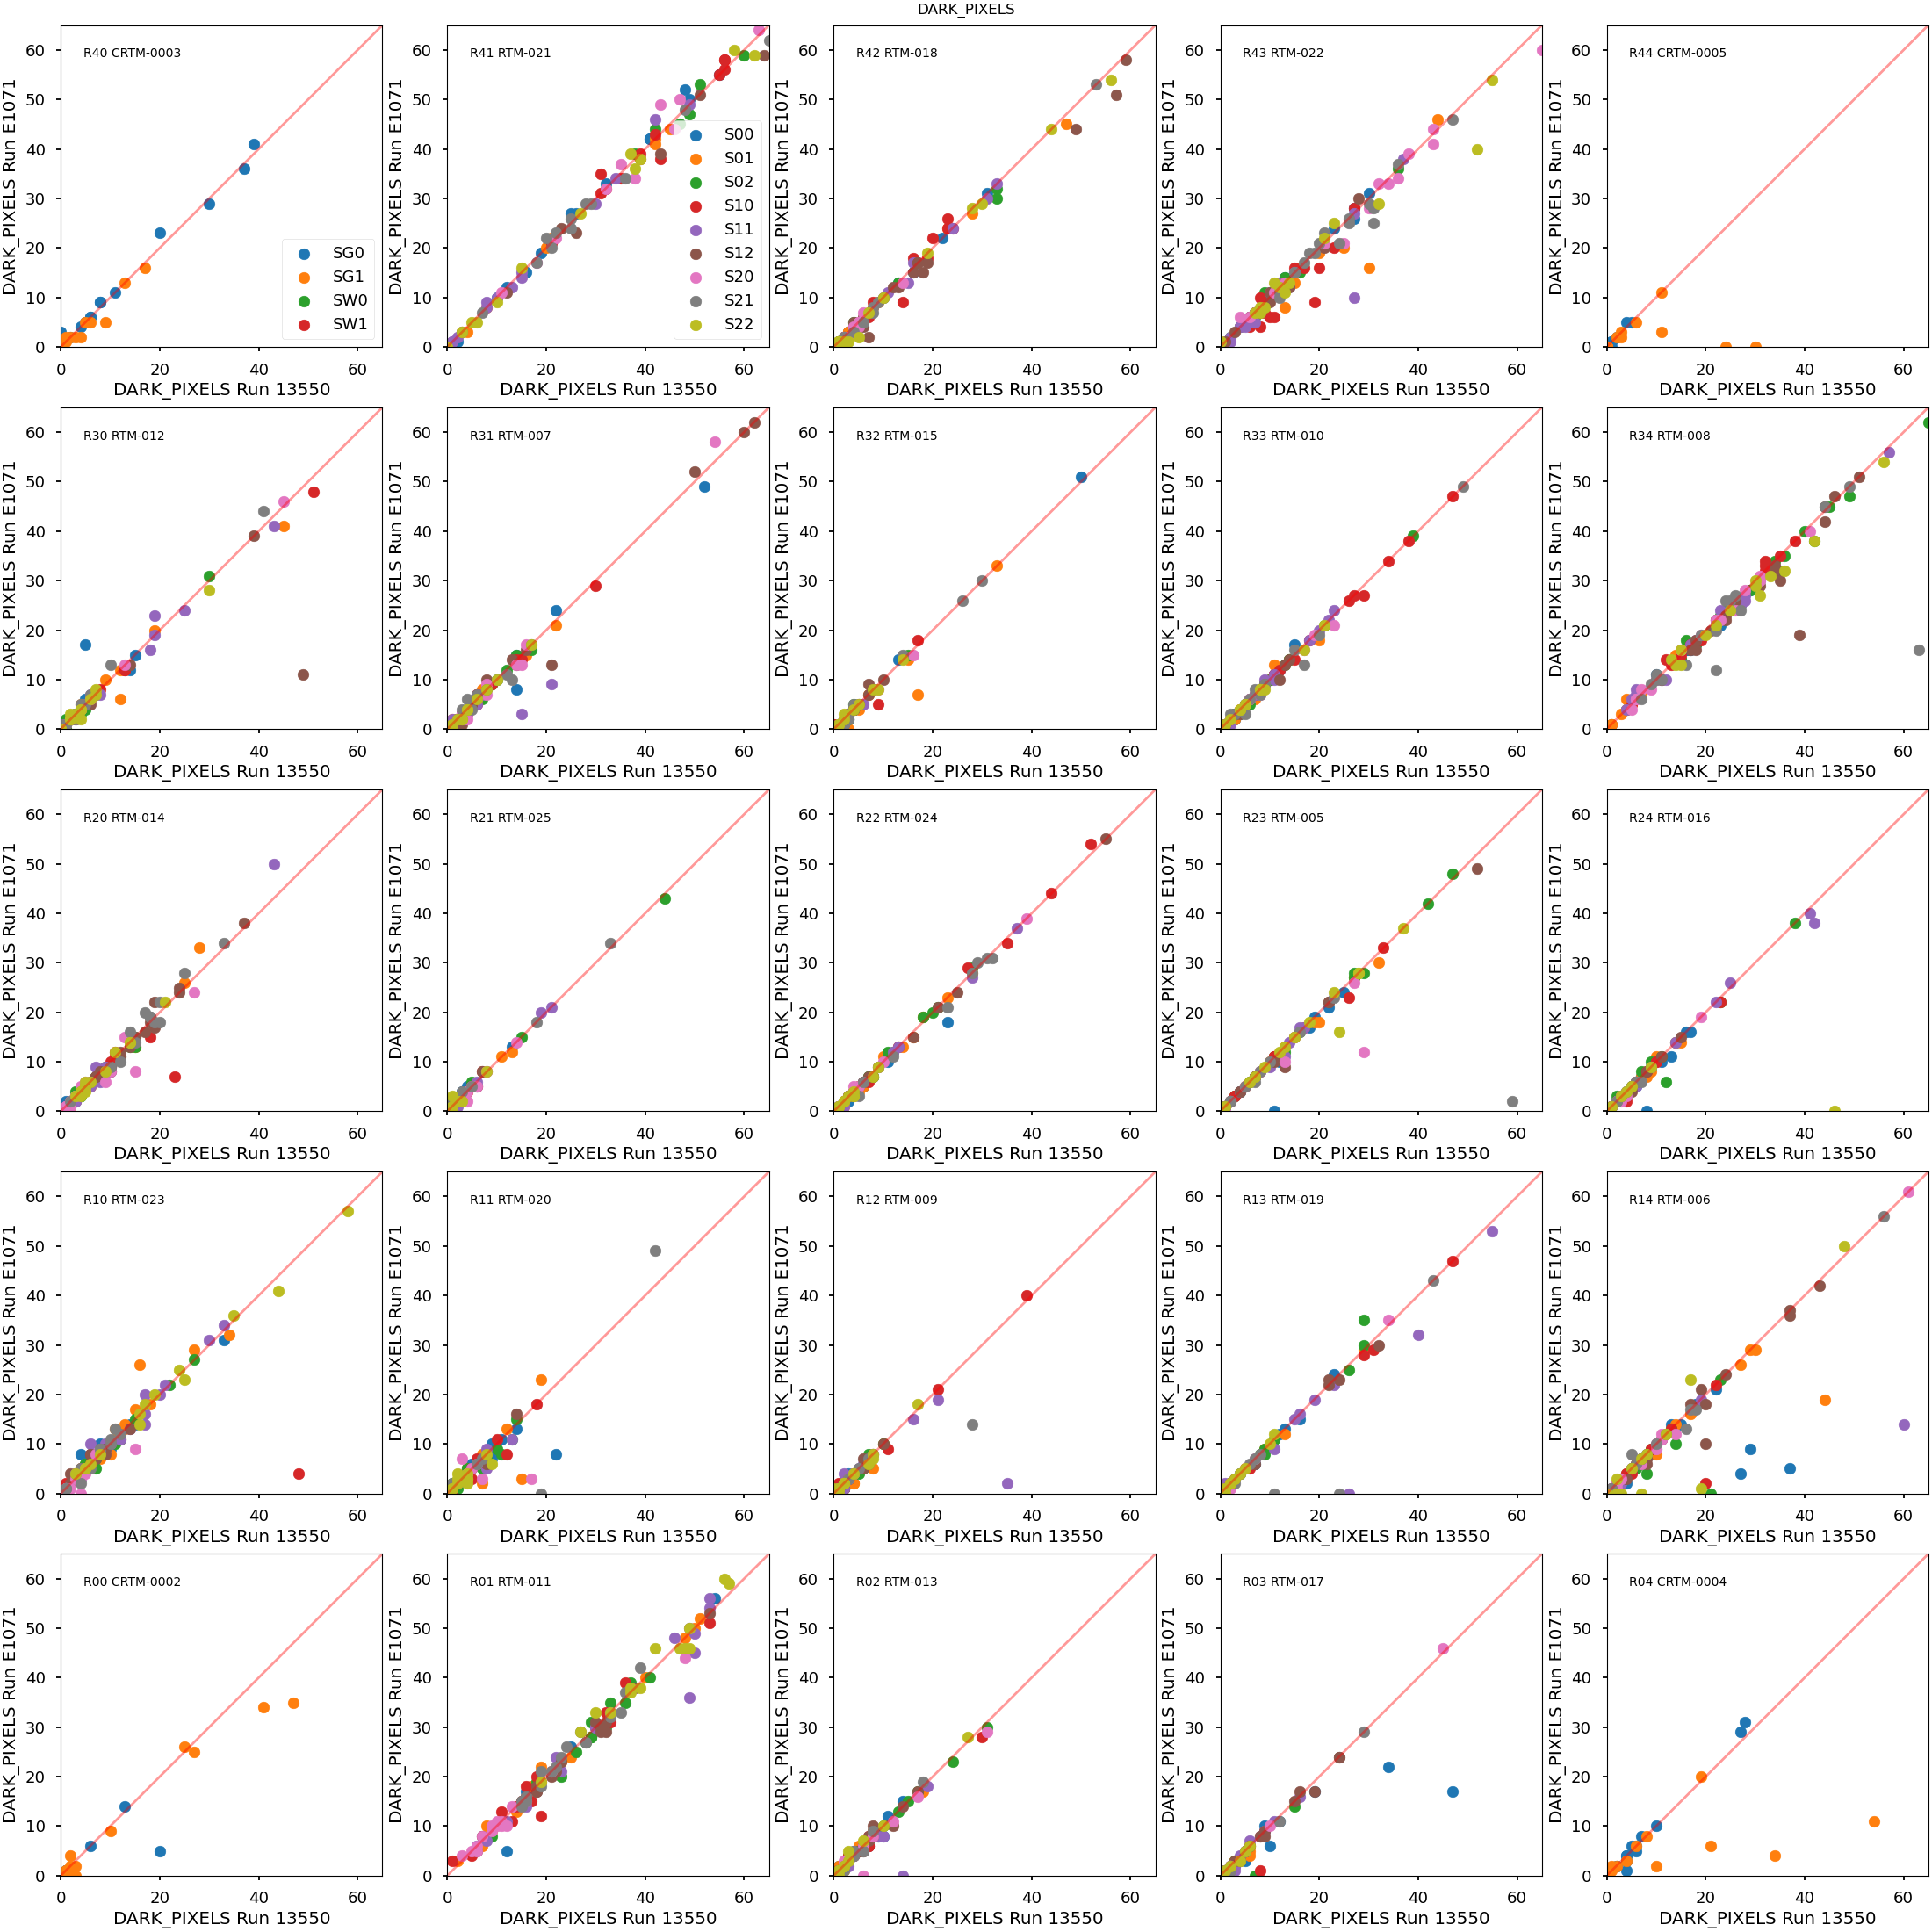
\includegraphics[width=0.7\textwidth]{figures/baselineCharacterization/13550_E1071_DARK_PIXELS_inset2.png}
\caption{Comparison of dark pixel counts in Run 7 (E1071) and Run 6 (13550), with separate plots for each raft.  Within each plot the color coding for all amplifier segments in a given CCD is the same.}
\label{fig:dark-pixels}
\end{centering}
\end{figure}

The default eo-pipe configuration has no border masking. The largest region permitted for the picture frame region is 9 pixels, determined by LCA-19363. Using a 9 pixel mask, the picture frame signal is removed, leaving true dark defects to be measured without contamination.

\begin{figure}[ht]
    \centering
    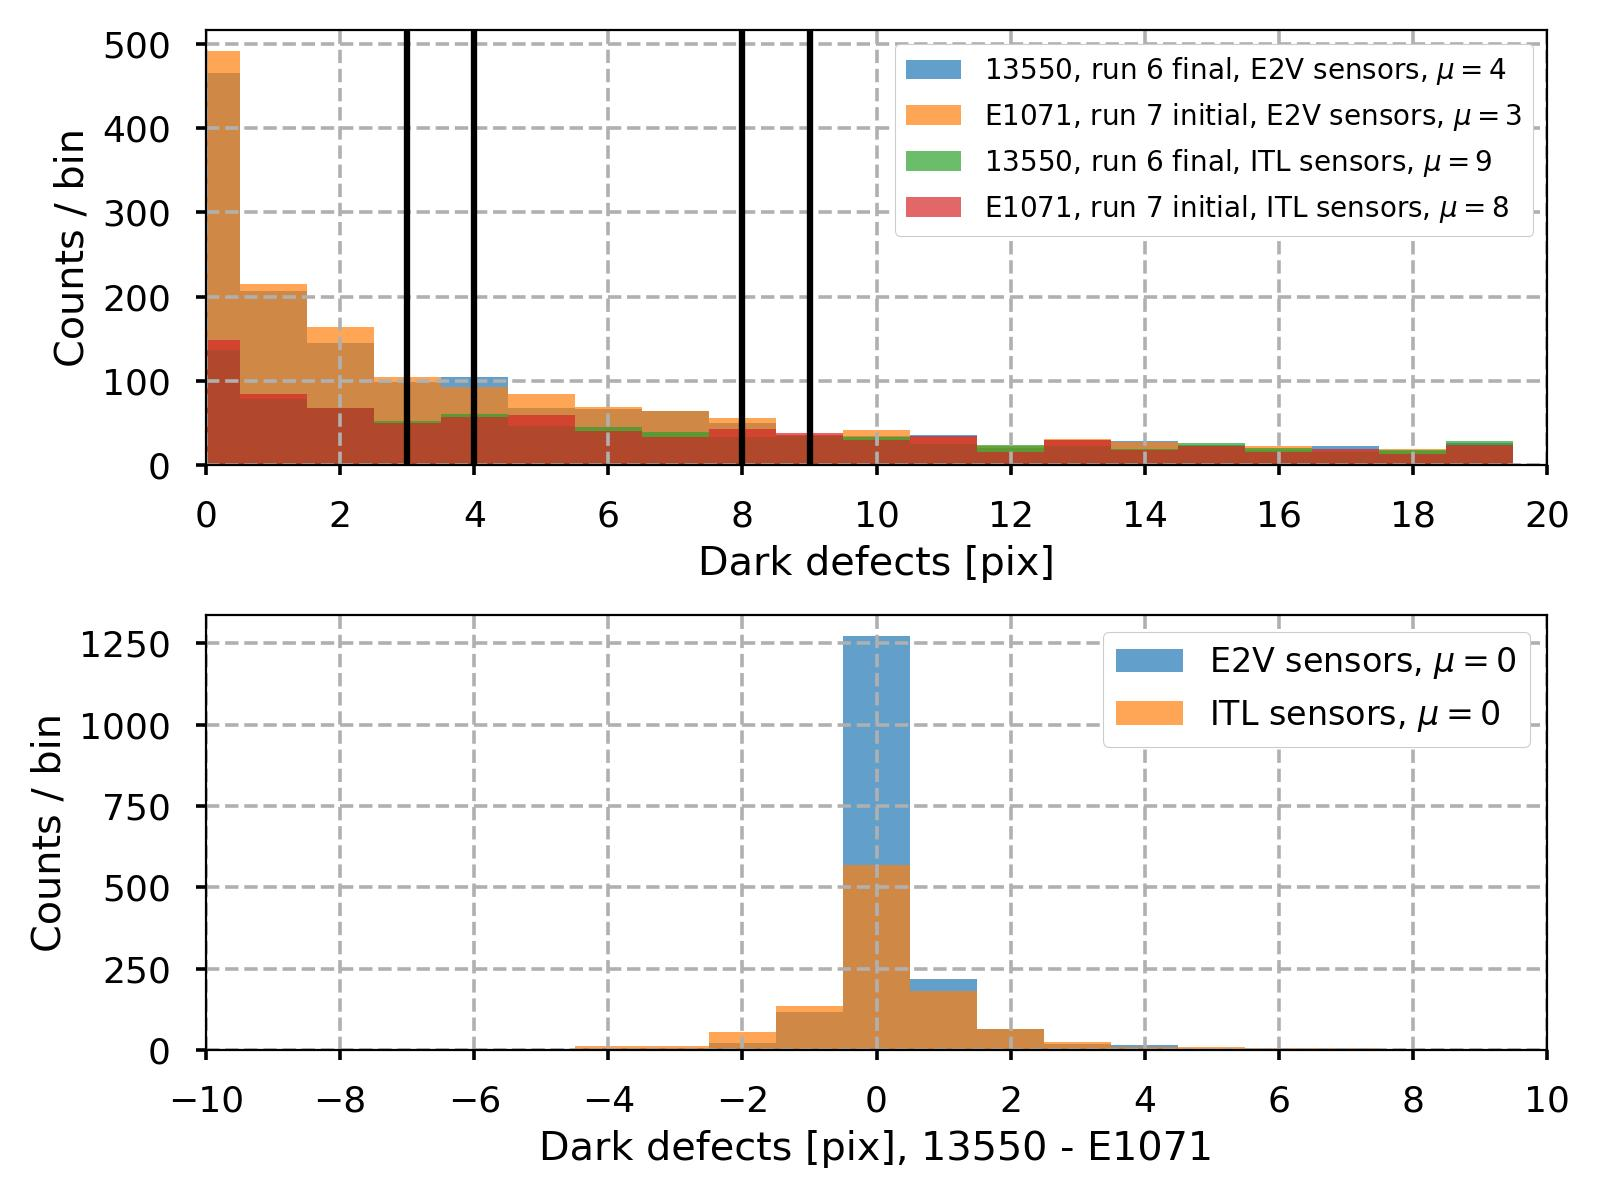
\includegraphics[width=0.7\linewidth]{figures/baselineCharacterization/darkDefects_comparison_initial.jpg}
    \caption{Comparison of dark pixel counts in Run 7 (E1071) and Run 6 (13550). Top: A histogram of amplifier measurements, separated by run number and sensor type. Bottom: A histogram of the amplifier dark pixel count differences, the difference is taken as the measurement from Run 6 and the measurement from Run 7.}
    \label{fig:initChar:DarkPixels:hists}
\end{figure}

In both instances, the contamination of dark pixels across the focal plane is \leq 10 pixels per amplifier on average. There is a measurable improvement in the dark pixel counts, decreasing by one pixel per amplifier between Run 6 and Run 7.

\clearpage
\subsection{Persistence}\label{sec:initPersistenceChar}

Persistence is a feature of CCDs and how they are operated involving charge trapped in the
surface layer after high-flux exposures \citep{dmtn-276,2024SPIE13103E..0WU}.
Persistence is described in detail in Section~\ref{sec:persistence-optimization}.
Here we consider the measurements taken as
part of a persistence measurement task in the typical B protocol. For
measuring persistence, a high-flux acquisition is taken, followed by a
sequence of dark images. The persistence signal has been observed to
decrease in subsequent dark images as the trapped charge is released (see Figure~\ref{fig:persistence-decay} for an example). As a metric for persistence,
we evaluate the difference between the residual ADU in the first dark
image and the average of the residual ADU in the final dark images. This residual signal is found to be \textasciitilde10 ADU.

\begin{figure}[ht]
\begin{centering}
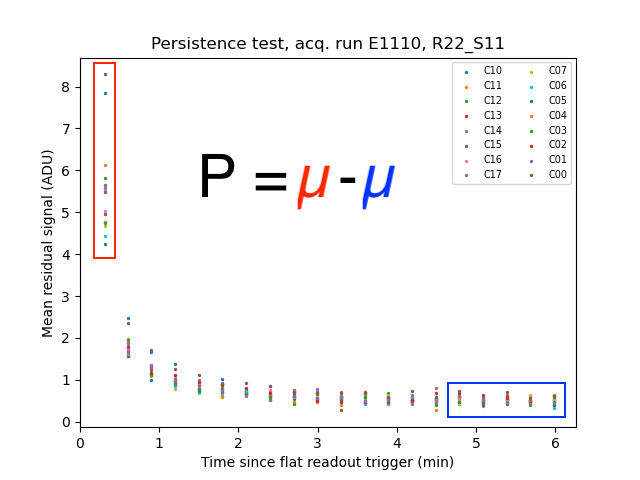
\includegraphics[width=0.7\textwidth]{figures/baselineCharacterization/persistence_plot_LSSTCam_R22_S11_u_lsstccs_eo_persistence_E1110_w_2024_35_20240926T235141Z.png}
\caption{Persistence signal observed in R22\_S11 in Run 7 (E1110) as a function of time after the high-flux flat image.  The color coding indicates the individual amplifier segments.  The persistence metric is defined as the residual signal in the first dark image after the flat acquisition (red box).  Note that over time the signal does not decay entirely to zero. This may be more due to bias fluctuation or incomplete image reduction. It definitely should return to 0 on some timescale.}
\label{fig:persistence-decay}
\end{centering}
\end{figure}

In the initial Run~7 measurements, we had not changed any operating
parameters of LSST Camera, so we would expect persistence to still be
present images at the same level as in Run~6.

\begin{figure}[ht]
\begin{centering}
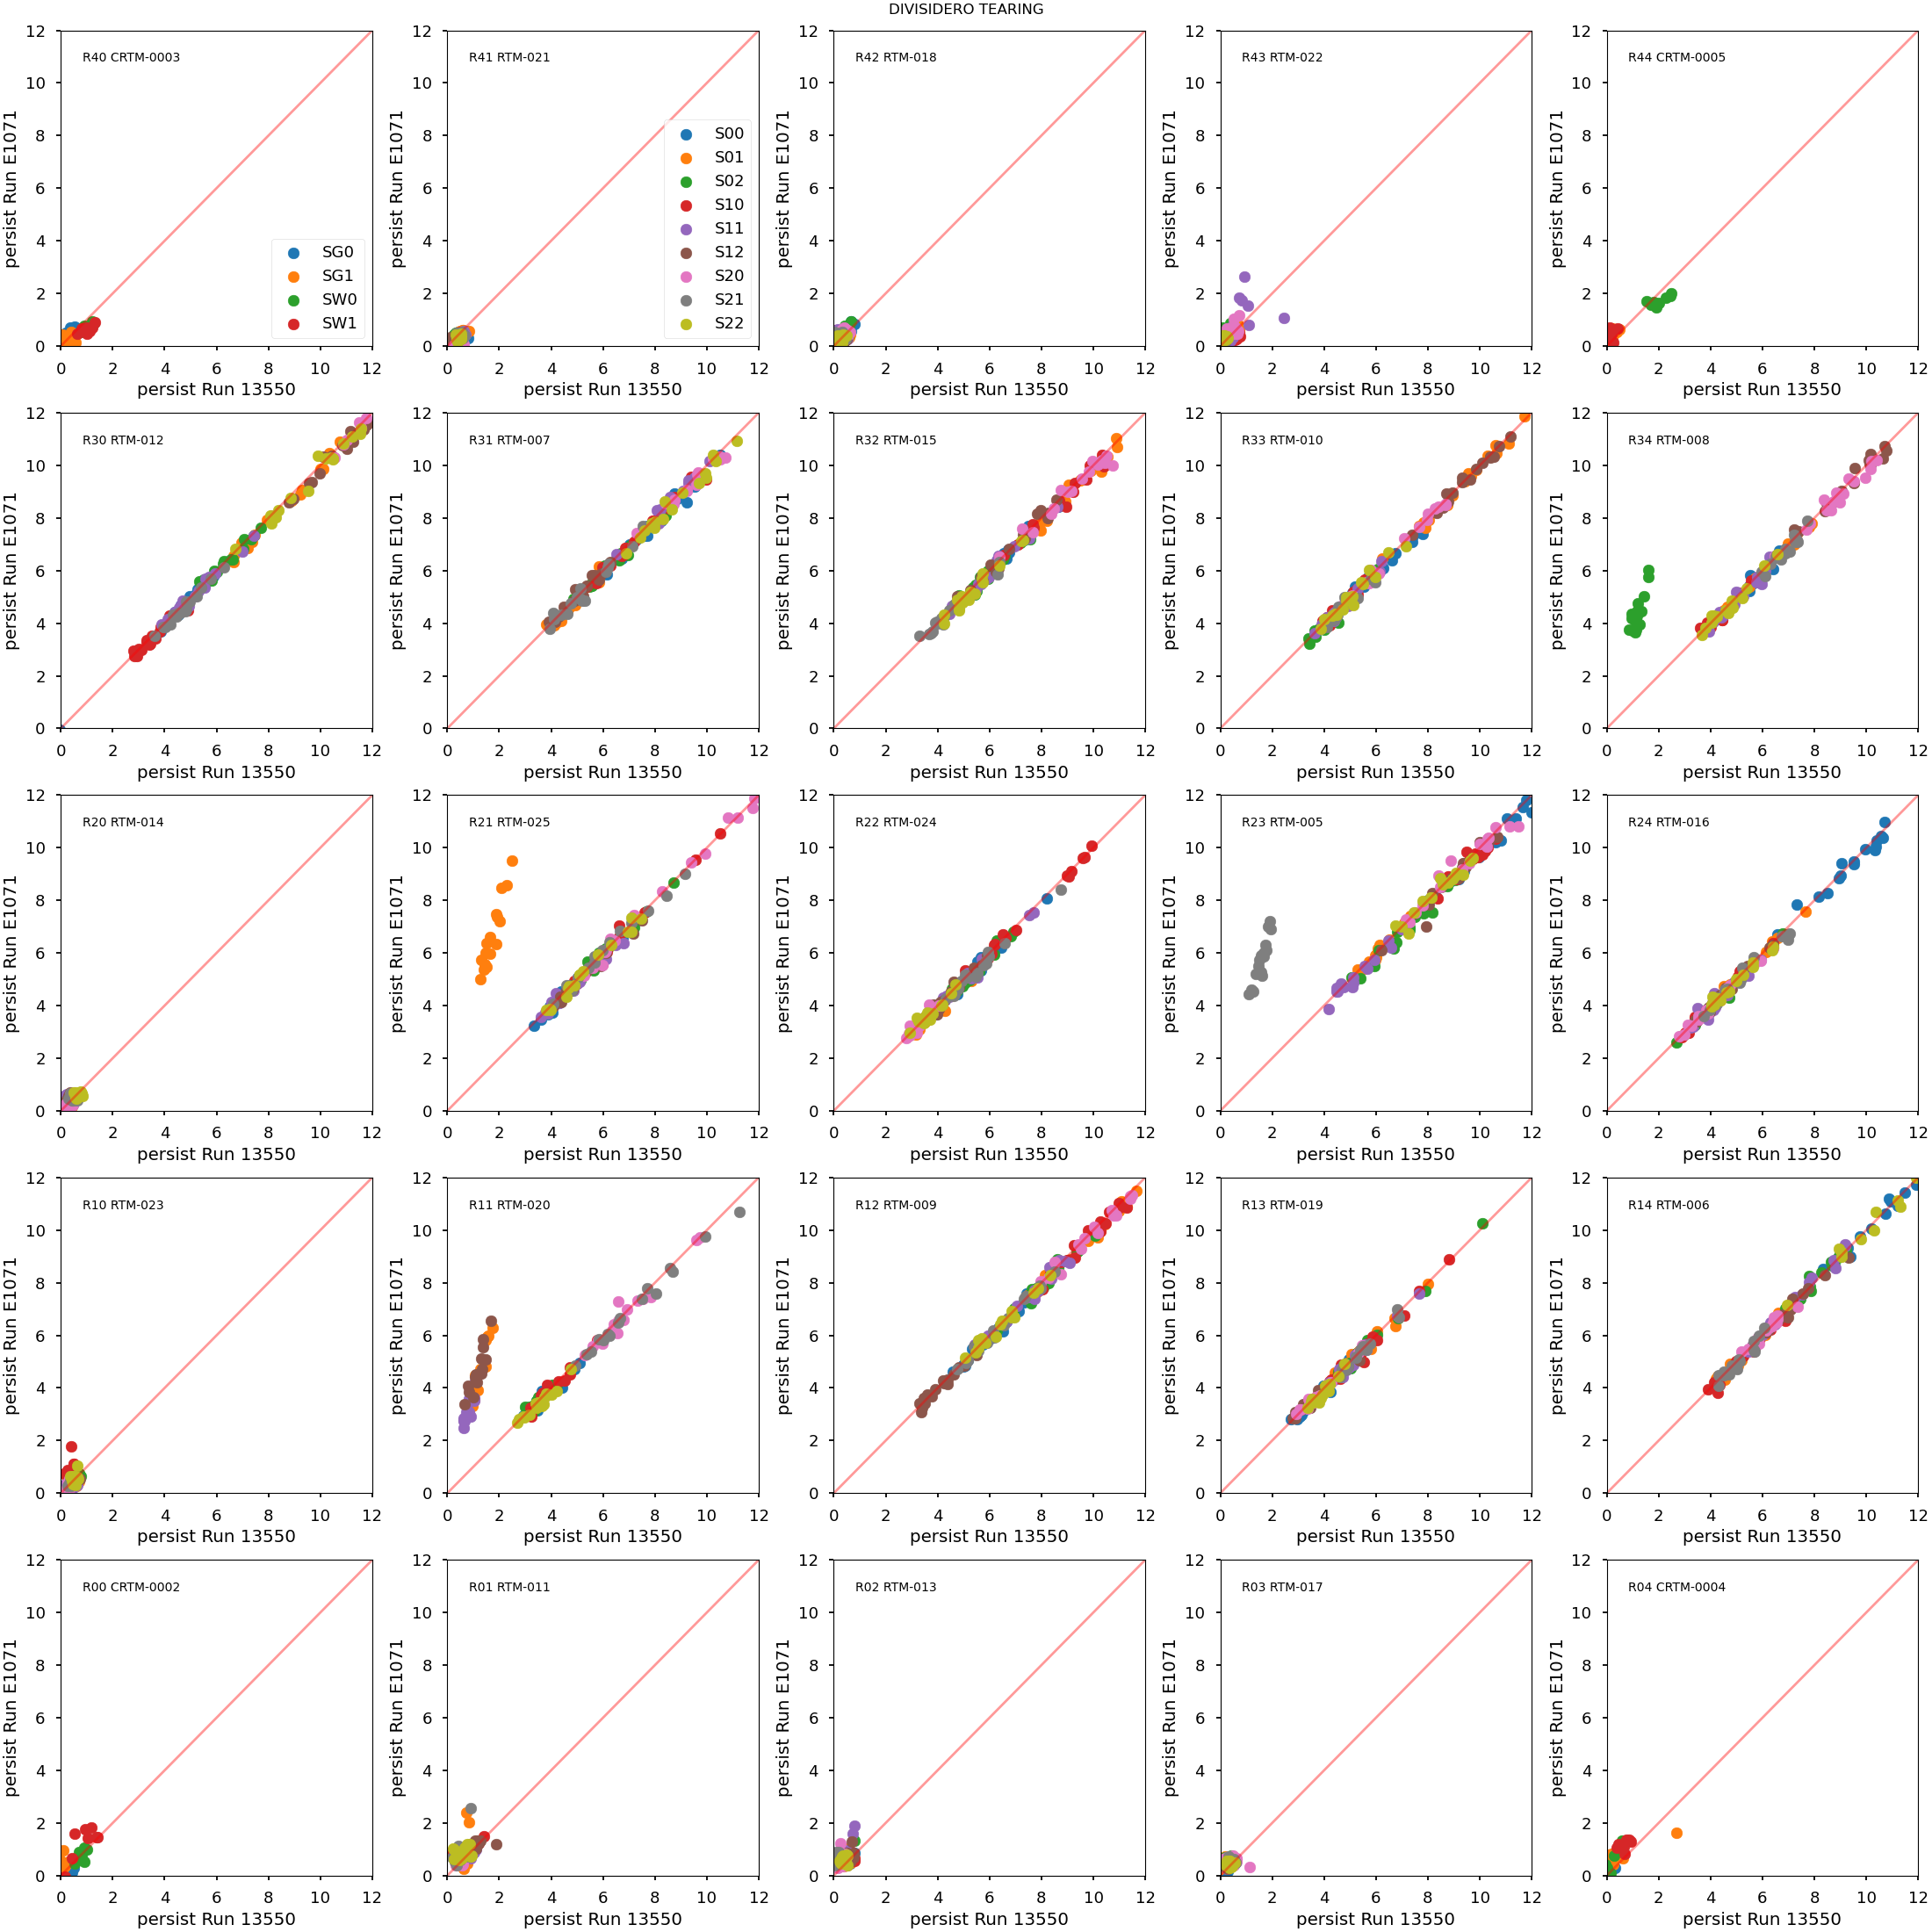
\includegraphics[width=0.7\textwidth]{figures/baselineCharacterization/13550_E1071_persist_inset.png}
\caption{Comparison of persistence metric between Run 7 (E1071) and Run 6 (13350), organized by raft.  The color coding indicates individual CCDs.  Several e2v CCDs have markedly greater persistence in Run 7.}
\label{fig:persistence-comp}
\end{centering}
\end{figure}

The persistence signal is generally consistent in e2v sensors between Run 6 and Run 7. Several e2v CCDs have greater persistence metric value in Run 7 (Fig.~\ref{fig:persistence-comp}). The outliers in
persistence measurements are due to higher initial residual ADU in a subset of rafts, resulting in an excess of \textasciitilde5 ADU when comparing Run 6 with Run 7 (see Fig.~\ref{fig:persistence-decay-comp}).


\begin{figure}[ht]
\centering
\begin{subfigure}{0.5\textwidth}
  \centering
  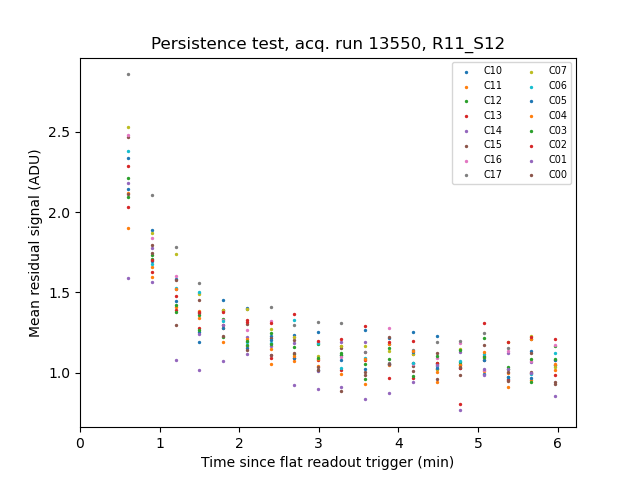
\includegraphics[width=1.0\textwidth]{figures/baselineCharacterization/persistence_plot_LSSTCam_R11_S12_u_lsstccs_eo_persistence_13550_w_2023_41_20231117T001459Z.png}
\end{subfigure}%
\begin{subfigure}{0.5\textwidth}
  \centering
  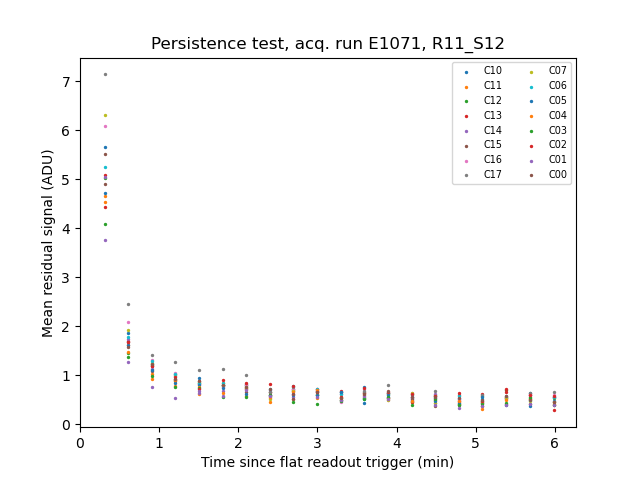
\includegraphics[width=1\textwidth]{figures/baselineCharacterization/persistence_plot_LSSTCam_R11_S12_u_lsstccs_eo_persistence_E1071_w_2024_35_20240925T180602Z.png}
\end{subfigure}
\caption{Comparison of persistence profiles for R12\_S21 between (left) Run 6 (13550) and (right) Run 7 (E1071).  The decay time constants are similar but the initial persistence level is greater in Run 7.  The asymptotic levels are also slightly different.}
\label{fig:persistence-decay-comp}
\end{figure}

\clearpage
\subsection{Differences between Run 6 and Run 7}\label{differences-from-previous-runs}

All camera performance metrics from the summit show close agreement with SLAC IR2 tests. PTC/full-well metrics were consistent, and no significant bright cosmetic defects developed. Dark cosmetic defects are difficult to quantify due to the edge sensor effects, though the consistency in CTI measurements would indicate that dark defects did not change from previous runs. Dark current and divisadero tearing show improved performance compared to Run 6, while the Persistence feature is still prominent in e2v sensors. 

\begin{table}[ht]
\centering
\resizebox{\textwidth}{!}{ % Resize the table to the page width
\begin{tabular}{|l|l|ll|ll|}
\hline
\multirow{2}{*}{Parameter [unit]} & \multirow{2}{*}{Specification} & \multicolumn{2}{l|}{e2v}                   & \multicolumn{2}{l|}{ITL}                    \\ \cline{3-6} 
                                   &                                & \multicolumn{1}{l|}{Run 6}     & Run 7     & \multicolumn{1}{l|}{Run 6}     & Run 7      \\ \hline
Serial CTI {[}\%{]}                & 5$\times 10^{-4}$               & \multicolumn{1}{l|}{3.7$\times 10^{-5}$} & 1.1$\times 10^{-5}$& \multicolumn{1}{l|}{1.2$\times 10^{-4}$} & 1.7$\times 10^{-4}$ \\ \hline
Parallel CTI {[}\%{]}              & 3$\times 10^{-4}$               & \multicolumn{1}{l|}{1.2$\times 10^{-5}$} & 1.2$\times 10^{-5}$& \multicolumn{1}{l|}{3.4$\times 10^{-7}$} & -4.8$\times 10^{-6}$\\ \hline
Dark current {[}e-/pix/s{]}        & None               & \multicolumn{1}{l|}{0.055} & 0.025& \multicolumn{1}{l|}{0.046} & 0.021 \\ \hline % Fix this one
Bright defects {[}count{]}         & None               & \multicolumn{1}{l|}{0}          & 0         & \multicolumn{1}{l|}{0}          & 0          \\ \hline
Linearity turnoff {[}e-{]}         & >90,000 e-               & \multicolumn{1}{l|}{156,000} & 168,000 & \multicolumn{1}{l|}{173,000} & 178,000  \\ \hline
PTC turnoff {[}e-{]}               & >90,000 e-               & \multicolumn{1}{l|}{126,000}  & 133,000  & \multicolumn{1}{l|}{117,000}  & 129,000   \\ \hline
PTC Gain {[}e- / ADU{]}            & None               & \multicolumn{1}{l|}{1.48}    & 1.48    & \multicolumn{1}{l|}{1.67}    & 1.68     \\ \hline
Read noise {[}e-{]}            & <9 e-               & \multicolumn{1}{l|}{5.30}    &   5.32  & \multicolumn{1}{l|}{6.20}    &  6.26    \\ \hline
PTC $a_{00}$ [$\frac{1}{pix^2}$]   & None               & \multicolumn{1}{l|}{3.09$\times 10^{-6}$} & 3.09$\times 10^{-6}$& \multicolumn{1}{l|}{1.71$\times 10^{-6}$} & 1.70$\times 10^{-6}$ \\ \hline
BF x-correlation                   & None               & \multicolumn{1}{l|}{0.524}    & 0.517    & \multicolumn{1}{l|}{0.716}    & 0.752     \\ \hline
BF y-correlation                   & None               & \multicolumn{1}{l|}{0.179}    & 0.170    & \multicolumn{1}{l|}{0.286}    & 0.287     \\ \hline
Row-means variance                 & None               & \multicolumn{1}{l|}{0.993}    & 0.884    & \multicolumn{1}{l|}{0.992}    & 0.947     \\ \hline
Dark defects {[}count{]}           & <2\%               & \multicolumn{1}{l|}{4} & 3 & \multicolumn{1}{l|}{9} & 8  \\ \hline
Divisadero tearing maximum {[}\%{]}& None               & \multicolumn{1}{l|}{0.327}   & 0.274   & \multicolumn{1}{l|}{0.752}   & 0.626    \\ \hline
Persistence {[}ADU{]}              & None               & \multicolumn{1}{l|}{5.67}    & 5.64    & \multicolumn{1}{l|}{0.48}   & 0.42    \\ \hline
\end{tabular}
}
\caption{Comparison of the median values of different parameters between Run 6 and Run 7, separated by detector type. For this comparison, only science detectors are considered.}\label{tab:initRever:Table}
\end{table}

\clearpage
